% La compilation de la présente documentation de la classe `yathesis' requiert :
%
% - une compilation `pdflatex` complète de `these.tex` situé dans le répertoire
% `../exemples/specimen/a-plat` avec le package `yathesis-demo` à charger en
% premier. le plus simple est de lancer `latexmk' comme suit :
%     latexmk -g -norc -r ./latexmkrc -jobname=these -pdflatex="pdflatex %O '\RequirePackage{etoolbox}\AtEndPreamble{\RequirePackage{yathesis-demo}}\input{%S}'" these.tex
% - une compilation `pdflatex` complète de `yathesis-fr.tex` comme suit :
%     latexmk -norc -r ./latexmkrc yathesis-fr
%
% Après compilation de la présente documentation, l'impression 2 pages sur 1
% peut se faire au moyen de :
% - complètement :
%     pdfnup --nup 2x1 --landscape yathesis-fr.pdf --suffix 2x1
% - partiellement (par exemple, pages 1 à 79 seulement) :
%     pdfnup --nup 2x1 --landscape yathesis-fr.pdf '1-79' --suffix 2x1
%
% Pour une impression papier, on pourra avoir (préalablement à la compilation)
% passé les options  :
% - `oneside' à la classe `yathesis' pour économiser le papier
% - `lscape' au package  `denisbdoc' pour éviter que les pages en paysage ne
%   soient imprimées en portrait.
%
\documentclass[version=final,noerror,localtocs]{yathesis}
\usepackage{ltxtable}%
\usepackage[yad]{denisbdoc}
\usepackage{dirtree}
\usepackage[lining]{libertine}
%
\lstset{%
  alsolanguage=[glossaries]TeX,%
  alsolanguage=[hyperref]TeX,%
}
%
\makeindex[title=Index des concepts,extout=pdx,extin=pnd,columnseprule]
%
\AtEndPreamble{%
  \changes{v1.0.2}{2020-04-13}{Documentation révisée}%
  \changes{v1.0.2}{2020-04-13}{Correction de bugs}%
  \changes{v1.0.0}{2020-03-26}{Documentation révisée}%
  \changes{v1.0.0}{2020-03-26}{Correction de bugs}%
  \changes{v0.99u}{2019-03-28}{Documentation révisée}%
  \changes{v0.99u}{2019-03-28}{Correction de bugs}%
  \changes{v0.99t}{2018-07-09}{Correction de bug}%
  \changes{v0.99s}{2018-06-22}{Correction de bug}%
  \changes{v0.99s}{2018-06-21}{Correction de bug}%
  \changes{v0.99r}{2018-06-02}{Correction de bugs}%
  \changes{v0.99q}{2018-05-04}{Suppression de fichiers inutiles sur le
    \glsxtrshort*{ctan} (aucun changement dans les fonctionnalités)}%
  \changes{v0.99q}{2018-04-10}{Correction de bugs}%
  \changes{v0.99p}{2016-12-08}{Documentation révisée}%
  \changes{v0.99o}{2016-10-30}{Suppression d'un warning inutile du
    \Package{iflang}}%
  \changes{v0.99o}{2016-10-30}{Documentation révisée}%
  \changes{v0.99o}{2016-10-30}{Correction de bugs}%
  \changes{v0.99n}{2016-06-11}{Documentation révisée}%
  \changes{v0.99m}{2016-05-22}{Documentation révisée}%
  \changes{v0.99m}{2016-05-22}{Documentation compilable au moyen de
    \hologo{pdfLaTeX}}%
  \changes{v0.99l}{2014-10-23}{Documentation révisée}%
  \changes{v0.99k}{2014-10-01}{Documentation révisée}%
  \changes{v0.99k}{2014-10-01}{Corrections de bugs}%
  \changes{v0.99j}{2014-07-18}{Documentation révisée}%
  \changes{v0.99j}{2014-07-18}{Corrections de bugs}%
  \changes{v0.99i}{2014-07-17}{Documentation révisée}%
  \changes{v0.99i}{2014-07-17}{Corrections de bugs}%
  \changes{v0.99h}{2014-07-14}{Documentation révisée}%
  \changes{v0.99h}{2014-07-14}{Corrections de bugs}%
  \changes{v0.99g}{2014-07-13}{Documentation révisée}%
  \changes{v0.99g}{2014-07-13}{Corrections de bugs}%
  \changes{v0.99c}{2014-06-06}{Corrections de bugs}%
  \changes{v0.99c}{2014-06-06}{Documentation révisée}%
  \changes{v0.99b}{2014-06-02}{Corrections de bugs}%
  \changes{v0.99a}{2014-06-02}{Corrections de bugs}%
  \changes{v0.99}{2014-05-18}{Corrections de bugs}%
}%
\begin{document}
\title[Documentation of the class \texorpdfstring{\yat}{yathesis}]{%
  Documentation de la classe \texorpdfstring{\yat}{yathesis}%
}
%
\subtitle[\version{\yathesisfileversion}]{\version{\yathesisfileversion}}
%
\author[denis.bitouze@univ-littoral.fr]{Denis}{Bitouzé}
%
\subject[LaTeX class whose basic purpose is to facilitate dissertations'
typesetting of theses prepared in France]{Classe LaTeX destinée à faciliter la
  rédaction des mémoires de thèses préparées en France}
%
\keywords{mémoire, thèse, \texorpdfstring{\LaTeX}{LaTeX}, classe}{dissertation, thesis, \texorpdfstring{\LaTeX}{LaTeX}, class}
%
\def\mysplit#1-#2-#3-{\def\myyear{#1}\def\mymonth{#2}\def\myday{#3}}
\def\splitdate#1{\expandafter\mysplit#1-}
\splitdate{\yathesisfiledate}

\date{\myday}{\mymonth}{\myyear}%
%
\maketitle[nofrontcover,frametitle={drop lifted shadow}]

%%% Local Variables:
%%% mode: latex
%%% TeX-master: "../yathesis-fr"
%%% End:

\restoregeometry
\tableofcontents
This document gives a quick, relatively minimal example of the use of
\texttt{uafthesis.cls}, while trying to show its features.

This section is contained in \texttt{abstract.tex}.

\mainmatter
\documentclass[12pt]{report}
\usepackage[utf8]{inputenc}
\usepackage[brazilian,brazil]{babel}
\usepackage{fancyhdr,setspace,float,graphicx,lscape,array,longtable,colortbl,amsmath,amssymb,booktabs,multirow,hyperref,pdfpages,tocloft,titlesec,lipsum,natbib}
\usepackage[sectionbib]{chapterbib}
\begin{document}
%***
\clearpage
\linenumbers % numeração de linhas
\modulolinenumbers[3] % numeração de linhas
%***
% Texto
%***
\chapter{Nam dui ligula}
%***
\lipsum[2-2] Nam dui ligula, fringilla a, euismod sodales, sollicitudin vel, wisi. Morbi
auctor lorem non justo \citep{lamport1986latex}.
\section{Euismod sodales}
\lipsum[2-3]
%*** APAGAR O EXEMPLO ACIMA







%*** REFERÊNCIAS
\bibliography{referencias.bib}
\bibliographystyle{apalike}
\end{document}

\chapter{Caractéristiques de la thèse}
\label{cha-caract-du-docum}%
\indexdef{caractéristiques de la thèse}%

Ce chapitre liste les commandes et options permettant de spécifier les données
caractéristiques de la thèse. La plupart d'entre elles sont ensuite affichées
en divers emplacements du mémoire :
\begin{itemize}
\item%
  \index{titre!de la thèse}%
  \index{couverture}%
  \index{première de couverture}%
  sur les pages de 1\iere{} de couverture et de titre(s), produites par la
  commande \refCom{maketitle} ;
\item\index{laboratoire}%
  sur l'éventuelle page dédiée au(x) laboratoire(s) où la thèse a été préparée,
  produite par la commande \refCom{makelaboratory} ;
\item\index{mot clé}%
  sur l'éventuelle page dédiée aux mots clés, produite par la commande
  \refCom{makekeywords} ;
\item\index{résumé}%
  sur la page dédiée aux résumés, produite par la commande \refCom{makeabstract} ;
\item\index{quatrième de couverture}%
  sur l'éventuelle 4\ieme{} de couverture, produite par la commande
  \refCom{makebackcover}.
\end{itemize}
Certaines de ces caractéristiques figurent également comme métadonnées du fichier
\pdf{} produit.

\section{Où spécifier les caractéristiques de la thèse ?}
\label{sec-lieu-de-saisie}%
\index{caractéristiques de la thèse!lieu de spécification}%

Les commandes permettant de définir les caractéristiques de la thèse peuvent être
saisies, au choix :
\begin{description}
\item[dans le fichier (maître) de la thèse :]\
  \begin{enumerate}
  \item soit dans son préambule ;
  \item soit dans son corps ;
    \begin{dbwarning}{Caractéristiques de la thèse à saisir \emph{avant}
        \protect\refCom*{maketitle}}{avant-maketitle}
    Si les caractéristiques de la thèse sont saisies dans le corps du fichier
    (maître) de la thèse, elles doivent nécessairement l'être \emph{avant} la
    commande \refCom{maketitle}.
  \end{dbwarning}
  \end{enumerate}
\item[dans un fichier dédié]
  \index{fichier!des caractéristiques de la thèse}%
  \index{dossier!de configuration}%
  % \item\label{characteristicsfile} dans un fichier dédié,
  à nommer \file{\characteristicsfile} et à placer dans un sous-dossier à nommer
  \folder{\configurationdirectory}. Ces fichier et sous-dossier \aside{tous
    deux prévus à cet effet} sont à créer au besoin mais ils sont fournis par le
  canevas de thèse \enquote{en arborescence} livré avec la classe, décrit
  \vref{sec-canevas-arborescence}.
  \begin{dbwarning}{Fichier de caractéristiques à ne pas importer manuellement}{}
    Le \File{\characteristicsfile} est \emph{automatiquement} importé par la
    \yatCl{} et il doit donc \emph{ne pas} être explicitement importé : on
    \emph{ne} recourra donc \emph{pas} à la commande
    |\input{|\file{\characteristicsfile}|}| (ou autre commande d'importation
    similaire à \docAuxCommand{input}).
  \end{dbwarning}
\end{description}

\section{Caractéristiques de titre}
\label{sec-proprietes-de-titre}

Cette section liste les commandes et options permettant de \emph{préparer} les
pages de 1\iere{} de couverture et de titre de la thèse\footnote{Sauf cas
  particulier, ces pages seront dans la suite appelées simplement
  \enquote{pages de titre}.}.

\subsection{Auteur, (sous-)titre, discipline, spécialité,
  date, sujet}\label{sec-caracteristiques}

Les commandes suivantes permettent de stipuler les auteur, titre et éventuel
sous-titre, champ disciplinaire, spécialité, date et sujet de la thèse. Toutes
ces données, sauf le sujet, figureront automatiquement sur les pages de
titre\footnote{En outre, les titres et éventuels sous-titres figureront sur les
  pages de résumé (cf. \vref{sec-abstract}) et de 4\ieme{} de couverture (cf.
  \vref{sec-quatr-de-couv}).}.
%
\begin{docCommand}[doc description=\mandatory]{author}{\oarg{adresse
      courriel}\marg{prénom}\marg{nom}}%
  \index{caractéristiques de la thèse!liste!auteur}%
  \indexdef{auteur}%
  \index{auteur!courriel}%
  \index{courriel}%
  \indexdef{courriel!auteur}%
  \indexsee{mail}{courriel}%
  \indexsee{email}{courriel}%
  Cette commande définit l'auteur de la thèse. Ses \meta{prénom} et
  \meta{nom} :
  \begin{itemize}
  \item figureront sur la ou les pages de titre ;
  \item%
    \index{lien hypertexte!courriel}%
    seront un lien hypertexte vers l'\meta{adresse courriel} si celle-ci est
    renseignée en argument optionnel ;
  \item apparaîtront aussi comme métadonnée \enquote{Auteur} du
    fichier \pdf{} de la thèse.
  \end{itemize}
  \begin{dbwarning}{Format des prénom et nom de l'auteur}{}
    \index{auteur!format}%
    \index{nom!format}%
    \index{prénom!format}%
    \index{format!nom}%
    \index{format!prénom}%
    On veillera à ce que :
    \begin{enumerate}
    \item les éventuels accents figurent dans les \meta{prénom} et
      \meta{nom};
    \item \index{caractéristiques de la thèse!liste!auteur}%
      \index{capitales}%
      \indexsee{majuscules}{capitales}%
      le \meta{nom} \emph{ne} soit \emph{pas} saisi en capitales (sauf pour la
      ou les majuscules) car il sera automatiquement composé en petites
      capitales.
    \end{enumerate}
  \end{dbwarning}
\end{docCommand}
%
\begin{docCommand}[doc description=\mandatory]{title}{\oarg{titre dans la langue
      secondaire}\marg{titre}}%
  \index{caractéristiques de la thèse!liste!titre}%
  \indexdef{titre!de la thèse}%
  Cette commande définit le \meta{titre} de la thèse. Celui-ci apparaît alors
  aussi comme métadonnée \enquote{Titre} du fichier \pdf{} de la thèse.
\end{docCommand}
%
\begin{docCommand}{subtitle}{\oarg{sous-titre dans la langue
      secondaire}\marg{sous-titre}}%
  \index{caractéristiques de la thèse!liste!sous-titre}%
  \indexdef{sous-titre de la thèse}%
  \index{titre!de la thèse!sous-titre}%
  Cette commande définit l'éventuel \meta{sous-titre} de la thèse.
\end{docCommand}
%
\begin{docCommand}[doc description=\mandatory]{academicfield}{\oarg{discipline dans la langue
      secondaire}\marg{discipline}}%
  \index{caractéristiques de la thèse!liste!discipline}%
  \indexdef{discipline}%
  Cette commande définit la \meta{discipline} \aside{ou champ disciplinaire}
  de la thèse. Celui-ci apparaît alors aussi comme métadonnée \enquote{Sujet} du
  fichier \pdf{} de la thèse, sauf si la commande \refCom{subject} est utilisée.
\end{docCommand}
%
\begin{docCommand}{speciality}{\oarg{spécialité dans la langue
      secondaire}\marg{spécialité}}%
  \index{caractéristiques de la thèse!liste!spécialité}%
  \indexdef{spécialité}%
  Cette commande définit la \meta{spécialité} (du champ
  disciplinaire) de la thèse.
\end{docCommand}
%
\begin{dbremark}{Titre, sous-titre, champ disciplinaire et spécialité dans la
    langue secondaire}{titre-supp}%
  \index{caractéristiques de la thèse!liste!langue}%
  \emph{Via} leur argument obligatoire, les commandes \refCom{title},
  \refCom{subtitle}, \refCom{academicfield} et \refCom{speciality} définissent
  les titre, sous-titre, champ disciplinaire et spécialité, \emph{dans la
    langue principale} de la thèse \aside*{par défaut le français}. Chacune de
  ces commandes admet un argument optionnel permettant de stipuler la donnée
  correspondante \emph{dans la langue secondaire} de la thèse \aside*{par
    défaut l'anglais\footnote{Les langues principale et secondaire de la thèse
      sont détaillées \vref{sec-langues}.}}.

  Dès lors qu'une au moins des ces commandes est employée avec son argument
  optionnel, la commande \refCom{maketitle}, qui produit les pages de titre
  composées dans la langue principale, génère \emph{automatiquement} une page
  de titre \emph{supplémentaire} composée dans la langue secondaire.
\end{dbremark}
%
\begin{docCommand}[doc description=\mandatory]{date}{\marg{jour}\marg{mois}\marg{année}}
  \index{caractéristiques de la thèse!liste!date de soutenance}%
  \index{date!de soutenance}%
  Cette commande définit la date de la soutenance.
\end{docCommand}
%
\begin{docCommand}{submissiondate}{\marg{jour}\marg{mois}\marg{année}}
  \index{caractéristiques de la thèse!liste!date de soumission}%
  \index{date!de soumission}%
  %
  \changes{v0.99k}{2014-10-01}{Nouvelle commande \protect\refCom{submissiondate}
    permettant de stipuler une date de soumission du mémoire aux rapporteurs}%
  %
  Cette commande définit la date de la soumission du mémoire (qui ne figure
  qu'en version \enquote{à soumettre}, cf. option \docValue{submitted*}
  \vref{sec-versions}). Ses arguments sont soumis aux mêmes contraintes que ceux
  de la commande \refCom{date} (cf. \vref{wa-format-date}).
\end{docCommand}
%
\begin{dbwarning}{Format des jour, mois et année des dates de
    soutenance et de soumission}{format-date}
  \index{date!format}%
  \index{format!date}%
  Les \meta{jour}, \meta{mois} et \meta{année} doivent être des nombres
  (entiers), \meta{jour} et \meta{mois} étant compris respectivement :
  \begin{itemize}
  \item entre |1| et |31| ;
  \item entre |1| et |12|.
  \end{itemize}
\end{dbwarning}
%
\begin{docCommand}{subject}{\oarg{sujet dans la langue
      secondaire}\marg{sujet de la thèse}}
   \index{caractéristiques de la thèse!liste!sujet}%
   \indexdef{sujet}%
  Cette commande définit le \meta{sujet de la thèse}.  Celui-ci ne figure nulle
  part dans la version papier du mémoire : il n'apparaît que comme métadonnée
  \enquote{Sujet} du fichier \pdf{} de la thèse. Si cette commande n'est pas
  employée, c'est le champ disciplinaire (commande \refCom{academicfield}) qui
  apparaît comme métadonnée \enquote{Sujet}.
\end{docCommand}

\begin{dbexample}{Auteur, (sous-)titre, discipline, spécialité, sujet, date}{}
   \indexex{caractéristiques de la thèse}%
  Les données principales d'une thèse peuvent être les suivantes.
  % \tcbset{listing options={deletekeywords={[2]title}}}
  \NoAutoSpacing%
\begin{preamblecode}[title=Par exemple dans le \File{\characteristicsfile},listing options={deletekeywords={author,title,subtitle,date},deletekeywords={[2]title},deletekeywords={[5]academicfield,speciality}}]
\author[aa@zygo.fr]{Alphonse}{Allais}
\title[Laugh's Chaos]{Le chaos du rire}
\subtitle[Chaos' laugh]{Le rire du chaos}
\academicfield[Mathematics]{Mathématiques}
\speciality[Dynamical systems]{Systèmes dynamiques}
\date{1}{1}{2015}
\subject{Rire chaotique}
\end{preamblecode}
\end{dbexample}

\subsection{Instituts et entités}\label{sec-entites}

Les instituts et entités dans lesquels \aside{ou grâce auxquels} la thèse
a été préparée sont définis et précisés au moyen des commandes et options
listés dans cette section. Ils figureront automatiquement sur la ou les pages
de titre\footnote{Le ou les laboratoires apparaissent en outre sur les pages
  dédiée aux laboratoires, de résumés et de 4\ieme{} de couverture.}.

\subsubsection{Définition}
%
\begin{docCommand}{comue}{\oarg{précision(s)}\marg{nom de la
      {\normalfont\ttfamily\glsxtrshort*{comue}}}}
   \index{caractéristiques de la thèse!liste!comue@\glsxtrshort{comue}}%
   \indexdef{comue@\glsxtrshort{comue}}%
  Cette commande définit la \gls{comue}. Celle-ci ne figure que par
  l'intermédiaire de ses logo et \glsxtrshort{url} spécifiés au moyen des clés
  \refKey{logo} et \refKey{url}.
\end{docCommand}
%
\begin{docCommand}[doc description=\mandatory]{institute}{\oarg{précision(s)}\marg{nom de
      l'institut}}
  \index{caractéristiques de la thèse!liste!institut principal}%
  \indexdef{institut}%
  \indexdef{institut!principal}%
  \indexsee{université}{institut}%
  \indexsee{école}{institut}%
  Cette commande définit l'institut (ou l'université, l'école, etc.), principal
  en cas de cotutelle.
\end{docCommand}
%
\begin{docCommand}{coinstitute}{\oarg{précision(s)}\marg{nom de
      l'institut}}
  \index{caractéristiques de la thèse!liste!institut de cotutelle}%
  \index{institut!de cotutelle}%
  \indexdef{cotutelle!institut}%
  Cette commande définit l'institut de cotutelle. Celle-ci ne
  devrait être employée qu'en cas de thèse cotutelle de nature
  \emph{internationale}.
\end{docCommand}
%
\begin{docCommand}{company}{\oarg{précision(s)}\marg{nom de l'entreprise}}
  \index{caractéristiques de la thèse!liste!entreprise}%
  \indexdef{entreprise}%
  \indexsee{thèse industrielle}{entreprise}%
  \indexsee{cifre@\glsxtrshort{cifre}}{entreprise}%
  Cette commande définit l'entreprise ayant (co)financé la thèse.
  Celle-ci ne devrait être employée qu'en cas de thèse industrielle (par
  exemple dans le cadre d'un dispositif \glsxtrshort{cifre}).
\end{docCommand}
%
\begin{docCommand}[doc description=\mandatory]{doctoralschool}{\oarg{précision(s)}\marg{nom de l'école
      doctorale}}
  \index{caractéristiques de la thèse!liste!école doctorale}%
  \indexdef{école doctorale}%
  Cette commande définit l'école doctorale.
\end{docCommand}
%
\begin{docCommand}[doc description=\mandatory]{laboratory}{\oarg{précision(s)}\marg{nom}\marg{adresse}}
  \index{caractéristiques de la thèse!liste!laboratoire}%
  \indexdef{laboratoire}%
  \index{laboratoire!nom}%
  \index{laboratoire!adresse}%
  Cette commande définit le nom et l'adresse du laboratoire.
\end{docCommand}
%
\begin{dbremark}{Changements de ligne dans l'adresse du laboratoire}{}
  Il est possible de composer l'\meta{adresse} du laboratoire sur plusieurs
  lignes au moyen de la commande |\\|.
\end{dbremark}
%
\begin{dbexample}{Instituts et entités}{}
  \indexex{laboratoire}%
  Si la thèse a été préparée au \gls{lmpa} de l'\gls{ulco}, on
  pourra recourir à :
  \NoAutoSpacing%
\begin{preamblecode}[listing options={deletekeywords={[5]institute,doctoralschool}}]
\comue{Université Lille Nord de France}
\institute{ULCO}
\doctoralschool{ED Régionale SPI 72}
\laboratory{LMPA}{%
  Maison de la Recherche Blaise Pascal \\
  50, rue Ferdinand Buisson            \\
  CS 80699                             \\
  62228 Calais Cedex                   \\
  France%
}
\end{preamblecode}
\end{dbexample}
%
\begin{dbremark}{Laboratoires multiples}{}
  \index{laboratoire!multiple}%
  Si la thèse a été préparée dans plusieurs laboratoires, il est possible de
  tous les spécifier en utilisant la commande \refCom{laboratory} autant de
  fois que nécessaire. Par convention, le laboratoire stipulé à la première
  \aside{et éventuellement seule} occurrence de la commande
  \refCom{laboratory} est le laboratoire \emph{principal}.

  En cas de laboratoires multiples, tous ne figurent pas systématiquement :
  \begin{itemize}
  \item sur les pages de titre, le seul laboratoire affiché est le
    laboratoire principal ;
  \item sur les pages de résumés et de 4\ieme{} de couverture
    (cf. \vref{sec-abstract,sec-quatr-de-couv}), par défaut seul le laboratoire
    principal est affiché (mais un nombre arbitraire de laboratoires peut être
    affiché grâce à la clé \refKey{numlaboratories}) ;
  \item sur la page \aside{facultative} qui leur est dédiée
    (cf. \vref{sec-laboratoires}), tous les laboratoires stipulés sont
    affichés.
  \end{itemize}
\end{dbremark}

\subsubsection{Précisions}
\index{caractéristiques de la thèse!précision}%

Toutes les commandes précédentes admettent un argument optionnel permettant
d'apporter sur les instituts ou entités des \meta{précisions} --- sous la forme
d'une liste \meta{clé}|=|\meta{valeur}.
%
\paragraph{Pour tout institut ou entité}

Les clés suivantes\syntaxeoptions{} sont valables pour tout institut ou entité.

\begin{docKey}{logo}{=\meta{fichier image}}{pas de valeur
    par défaut, initialement vide}
  \indexdef{logo}%
  \index{laboratoire!logo}%
  \index{institut!logo}%
  Cette option définit le logo d'un institut, spécifié sous la forme de (du
  chemin menant à) son \meta{fichier image}.
  \begin{dbexample}{Logo d'institut}{logoinst}
    Supposons que la thèse ait été préparée à l'\gls{ulco} et qu'on dispose du
    logo de cette université sous la forme d'un fichier nommé
    \texttt{ulco.pdf}, situé dans le sous-dossier \folder{images}. On
    saisira alors :
\begin{preamblecode}[listing options={deletekeywords={[5]institute}}]
\institute[logo=images/ulco]{ULCO}
\end{preamblecode}
\end{dbexample}
Tous les logos apparaissent automatiquement en haut de la ou des
pages de titre, sauf :
\begin{itemize}
\item ceux des laboratoires qui ne figurent que sur l'éventuelle page qui leur
  est dédiée ;
\item celui de l'école doctorale qui ne figure nulle part et qu'il est donc
  inutile de spécifier.
\end{itemize}
\end{docKey}
%
\begin{docKey}{logoheight}{=\meta{dimension}}{pas de valeur par
    défaut, initialement \docValue*{1.5cm}}
  \indexdef{logo!taille}%
  \indexdef{taille!logo}%
  Par défaut, tous les logos ont une même hauteur de \SI{1.5}{\cm}
  mais la clé \refKey{logoheight} permet de spécifier une hauteur
  différente.
  \begin{dbexample}{Hauteur du logo d'institut}{}
    La commande de l'\vref{ex-logoinst} aurait ainsi pu contenir :
\begin{preamblecode}[listing options={deletekeywords={[5]institute}}]
\institute[logoheight=1cm,logo=images/ulco]{ULCO}
\end{preamblecode}
\end{dbexample}
\end{docKey}
%
\begin{docKey}[][doc new=2019-03-28]{nologo}{=\docValue{true}\textbar\docValue{false}}{par défaut
    \docValue{true}, initialement \docValue{false}}%
  %
  \indexdef{logo!suppression}%
  \changes{v0.99u}{2019-03-28}{Nouvelle option \protect\refKey{nologo} des
    commandes d'instituts et entreprise permettant de (légèrement) personnaliser
    les pages de titre}%
  %
  Si les commandes \refCom{comue}, \refCom{institute}, \refCom{coinstitute} et
  \refCom{company} sont employées sans l'option \refKey{logo}, les zones des
  pages de titre réservées aux logos correspondants contiennent les rappels
  respectivement \enquote{\meta{logo ComUE}}, \enquote{\meta{logo de
      l’institut}}, \enquote{\meta{logo de l’institut de cotutelle}} et
  \enquote{\meta{logo de l’entreprise}}. Si l'option \refKey{logo} est absente
  parce que l'affichage du logo correspondant n'est pas souhaité, l'option
  \refKey{nologo} permet de supprimer ce rappel.
\end{docKey}
%
\begin{docKey}{url}{=\meta{{\normalfont\ttfamily\glsxtrshort*{url}} de
      l'institut}}{pas de valeur par défaut, initialement vide}
  \indexdef{url@\glsxtrshort{url}}%
  \index{laboratoire!url@\glsxtrshort{url}}%
  \index{institut!url@\glsxtrshort{url}}%
  \index{lien hypertexte}%
  Cette option définit l'\glsxtrshort{url} d'un institut. Les noms et éventuels
  logos des instituts sont alors des liens hypertextes pointant vers cette
  \glsxtrshort{url}.
  \begin{dbexample}{\glsxtrshort*{url} d'institut}{}
    Si la thèse a été préparée à l'\gls{ulco}, on pourra recourir à :%
    \NoAutoSpacing%
\begin{preamblecode}[listing
options={deletekeywords={url},morekeywords={[2]url},deletekeywords={[5]institute}}]
\institute[url=http://www.univ-littoral.fr/]{ULCO}
\end{preamblecode}
\end{dbexample}
%
\begin{dbwarning}{Caractère \protect\lstinline+\#+ à protéger dans les
    \glsxtrshortpl*{url} d'instituts et entités}{}
  \index{url@\glsxtrshort{url}!format}%
  \index{format!url@\glsxtrshort{url}}%
  Au cas (peu probable) où le caractère |#| doive figurer dans ces
  \glsxtrshortpl{url}, il doit être \enquote{protégé} au moyen d'une
  contre-oblique le précédant : |\#|.
\end{dbwarning}
\end{docKey}

\paragraph{Pour le laboratoire seulement}
  \index{caractéristiques de la thèse!liste!laboratoire}%

Les options supplémentaires suivantes \emph{ne} sont prévues
\emph{que} pour l'entité \enquote{laboratoire} qui, contrairement
aux autres, peut disposer d'une page dédiée\pagededieelabo.
%
\begin{docKey}{telephone}{=\meta{numéro}}{pas de valeur par défaut,
    initialement vide}
  \indexdef{téléphone}%
  \index{laboratoire!téléphone}%
  Cette option définit le numéro de téléphone du laboratoire.
\end{docKey}
%
\begin{docKey}{fax}{=\meta{numéro}}{pas de valeur par défaut,
    initialement vide}
  \indexdef{fax}%
  \index{laboratoire!fax}%
  Cette option définit le numéro de fax du laboratoire.
\end{docKey}
%
\begin{docKey}{email}{=\meta{adresse courriel}}{pas de valeur par
    défaut, initialement vide}
  \index{courriel}%
  \indexdef{courriel!laboratoire}%
  \index{laboratoire!courriel}%
  Cette option définit l'adresse courriel du laboratoire.
\end{docKey}
%
\begin{docKey}{nonamelink}{=\docValue{true}\textbar\docValue{false}}{par défaut
    \docValue{true}, initialement \docValue{false}}
  \changes{v0.99i}{2014-07-17}{Nouvelle option \protect\refKey{nonamelink}
    agissant sur les hyperliens des laboratoires}%
  \index{lien hypertexte!suppression}%
  \indexsee{hyperlien}{lien hypertexte}%
%
  Cette option a pour effet que, si l'\glsxtrshort{url} du laboratoire a été
  définie au moyen de l'option \refKey{url}, le nom de celui-ci n'est pas un
  lien hypertexte : seuls l'\glsxtrshort{url} en regard de la mention du site Web
  et l'éventuel logo figurant la page dédiée aux laboratoires\pagededieelabo{}
  sont des liens hypertextes pointant vers cette \glsxtrshort{url}.
\end{docKey}
%
\begin{dbexample}{Laboratoire}{}
  \indexex{laboratoire}%
  Si la thèse a été préparée au \gls{lmpa}, on peut recourir à :
  \NoAutoSpacing%
\begin{preamblecode}[listing options={deletekeywords={url},morekeywords={[2]url}}]
\laboratory[
telephone=(33) 03 21 46 55 86,
fax=(33) 03 21 46 55 75,
email=secretariat@lmpa.univ-littoral.fr,
url=http://www-lmpa.univ-littoral.fr/
]{LMPA}{%
  Maison de la Recherche Blaise Pascal \\
  50, rue Ferdinand Buisson            \\
  CS 80699                             \\
  62228 Calais Cedex                   \\
  France%
}
\end{preamblecode}
\end{dbexample}
%
\begin{dbremark}{Téléphone, fax et courriel : pour le
    laboratoire seulement}{}
  Spécifier les options \refKey{telephone}, \refKey{fax}, \refKey{email} et
  \refKey{nonamelink} pour un autre institut que le laboratoire est inutile :
  ces précisions complémentaires n'auront aucun effet.
\end{dbremark}
%
\begin{dbremark}{Instituts sous forme d'acronymes}{acronymes}
  \index{acronyme}%
  \indexsee{sigle}{acronyme}%
  Si l'institut ou l'entité doit figurer sous la forme d'un acronyme, on aura
  intérêt à ne pas les saisir tels quel comme on l'a fait jusqu'ici
  (\lstinline[deletekeywords={[5]institute}]|\institute{ULCO}| ou
  |\laboratory{LMPA}|) mais à recourir aux fonctionnalités du
  \Package{glossaries}. L'\vref{acronymes} donne un aperçu de la procédure.
\end{dbremark}

\subsection{Directeur(s) de thèse et membres du jury}\label{sec-jury}

Les directeur(s) et membres du jury de la thèse sont définis et précisés au
moyen des commandes et options listés dans cette section. Ils figurent
automatiquement sur la ou les pages de titre\footnote{En versions \enquote{à
    soumettre} aux rapporteurs (cf. valeurs \protect\docValue{submitted} et
  \protect\docValue{submitted*} de la clé \protect\refKey{version}), les
  membres du jury ne figurent pas car le doctorant ne peut alors préjuger d'un
  jury, ne sachant pas encore s'il va être autorisé à soutenir.}.

\subsubsection{Définition}\label{sec-definition-directeurs-jury}

\paragraph{Directeurs}\label{sec-definition-directeurs}
\index{rôle!prédéfini}%

Parmi la ou les personnes assurant l'encadrement de la thèse,
celles ayant les rôles :
\begin{itemize}
\item de directeur  ;
\item de co-directeur ;
\item de co-encadrant ;
\end{itemize}
sont distinguées au moyen des commandes respectives \refCom{supervisor},
\refCom{cosupervisor} et \refCom{comonitor}, en versions éventuellement étoilées
pour désigner celles qui ne sont pas membres du jury.%
%
\changes{v0.99f}{2014-07-11}{Nouvelles commandes \protect\refCom{supervisor*},
  \protect\refCom{cosupervisor*} et \protect\refCom{comonitor*} permettant de
  spécifier des directeurs de thèses non membres du jury}%
%
\begin{docCommand}[doc
  description=\mandatory]{supervisor}{\oarg{précision(s)}\marg{prénom}\marg{nom}}
  \index{caractéristiques de la thèse!liste!directeur de thèse}%
  \indexdef{directeur de thèse}%
  \index{membre du jury!directeur de thèse}%
  Cette commande définit un directeur de la thèse (également membre du jury).
\end{docCommand}

\begin{docCommand}[doc description=\mandatory]{supervisor*}{\oarg{précision(s)}\marg{prénom}\marg{nom}}
  \index{caractéristiques de la thèse!liste!directeur de thèse}%
  \indexdef{directeur de thèse}%
  Cette commande définit un directeur de la thèse (non membre du jury).
\end{docCommand}

\begin{docCommand}{cosupervisor}{\oarg{précision(s)}\marg{prénom}\marg{nom}}
  \index{caractéristiques de la thèse!liste!co-directeur de thèse}%
  \indexdef{co-directeur de thèse}%
  \index{membre du jury!co-directeur de thèse}%
  Cette commande définit un éventuel co-directeur de la thèse (également membre du jury).
\end{docCommand}

\begin{docCommand}{cosupervisor*}{\oarg{précision(s)}\marg{prénom}\marg{nom}}
  \index{caractéristiques de la thèse!liste!co-directeur de thèse}%
  \indexdef{co-directeur de thèse}%
  Cette commande définit un éventuel co-directeur de la thèse (non membre du jury).
\end{docCommand}

\begin{docCommand}{comonitor}{\oarg{précision(s)}\marg{prénom}\marg{nom}}
  \index{caractéristiques de la thèse!liste!co-encadrant de thèse}%
  \indexdef{co-encadrant de thèse}%
  \index{membre du jury!co-encadrant de thèse}%
  Cette commande définit un éventuel co-encadrant de la thèse (également membre du jury).
\end{docCommand}

\begin{docCommand}{comonitor*}{\oarg{précision(s)}\marg{prénom}\marg{nom}}
  \index{caractéristiques de la thèse!liste!co-encadrant de thèse}%
  \indexdef{co-encadrant de thèse}%
  Cette commande définit un éventuel co-encadrant de la thèse (non membre du jury).
\end{docCommand}

\paragraph{Membres du jury}\label{sec-definition-jury}
\index{membre du jury}%
\indexsee{jury}{membre du jury}%

\begin{docCommand}{referee}{\oarg{précision(s)}\marg{prénom}\marg{nom}}
  \index{caractéristiques de la thèse!liste!rapporteur}%
  \indexdef{rapporteur de la thèse}%
  \index{membre du jury!rapporteur}%
  Cette commande définit un rapporteur de la thèse.
\end{docCommand}

\begin{docCommand}{committeepresident}{\oarg{précision(s)}\marg{prénom}\marg{nom}}
  \index{caractéristiques de la thèse!liste!président du jury}%
  \indexdef{président du jury}%
  \index{membre du jury!président}%
  \index{rôle!prédéfini}%
  Cette commande définit le président du jury de la thèse (dont le rôle figure
  sur la ou les pages de titre).
\end{docCommand}

\begin{docCommand}{examiner}{\oarg{précision(s)}\marg{prénom}\marg{nom}}
  \index{caractéristiques de la thèse!liste!examinateur}%
  \indexdef{examinateur}%
  \index{membre du jury!examinateur}%
  Cette commande définit un examinateur ordinaire de la thèse.
\end{docCommand}

\begin{docCommand}{guest}{\oarg{précision(s)}\marg{prénom}\marg{nom}}
  \index{caractéristiques de la thèse!liste!invité}%
  \indexdef{invité}%
  \index{membre du jury!invité}%
  Cette commande définit une éventuelle personne invitée au jury de la thèse.
\end{docCommand}
%
\begin{dbwarning}{Usage multiple et facultatif des commandes du
    jury}{}
  Toutes ces commandes sont à utiliser :
  \begin{description}
  \item[autant de fois que nécessaire :]
    \refCom{referee} et \refCom{examiner} (par exemple) seront
    certainement employées à plusieurs reprises ;
  \item[seulement si nécessaire :]
    \refCom{cosupervisor}, \refCom{comonitor} et \refCom{guest} (par
    exemple) peuvent ne pas être employées.
  \end{description}
  La commande \refCom{supervisor} (ou sa variante étoilée), utilisable elle
  aussi plusieurs fois, doit être employée au moins une fois.
\end{dbwarning}

\begin{dbexample}{Jury}{}
  \indexex{membre du jury}%
\begin{preamblecode}[listing options={deletekeywords={[5]supervisor,cosupervisor,committeepresident}}]
\supervisor{Michel}{de Montaigne}
\cosupervisor{Étienne}{de la Boétie}
%
\referee{René}{Descartes}
\referee{Denis}{Diderot}
%
\committeepresident{Victor}{Hugo}
\examiner{Charles}{Baudelaire}
\examiner{Émile}{Zola}
\examiner{Paul}{Verlaine}
%
\guest{George}{Sand}
\end{preamblecode}
\end{dbexample}

\begin{dbwarning}{Format des prénoms et noms des directeurs de thèse et membres du jury}{}
  \index{directeur de thèse!format}%
  \index{membre du jury!format}%
  \index{nom!format}%
  \index{prénom!format}%
  \index{format!nom}%
  \index{format!prénom}%
  Comme pour les prénom et nom de l'auteur de la thèse, on veillera à ce que :
  \begin{enumerate}
  \item les éventuels accents figurent dans les \meta{prénom} et \meta{nom};
  \item les \meta{nom} \emph{ne} soient \emph{pas} saisis en capitales (sauf
    pour la ou les majuscules) car ils seront automatiquement composés en
    petites capitales.
  \end{enumerate}
\end{dbwarning}

\subsubsection{Précisions}\label{sec-options-staff}

Toutes les commandes précédentes admettent un argument optionnel permettant
d'apporter sur les directeurs de thèse et membres du jury\footnote{Pour les
  directeurs de thèse \emph{non} membres du jury, ces \meta{précisions} sont
  inutiles car elles ne figureront nulle part.}
des \meta{précisions} :
\begin{enumerate}
\item corporation ;
\item affiliation ;
\item homme/femme.
\end{enumerate}
% --- sous la forme d'une liste \meta{clé}|=|\meta{valeur}.

\paragraph{Corporation}
\label{sec-corps}%
\indexsee{corps de métier}{corporation}%
\index{caractéristiques de la thèse!liste!corporation}%
\indexsee{fonction}{corporation}%
\indexsee{grade}{corporation}%
\index{corporation}%
\index{corporation!prédéfinie}%
\index{directeur de thèse!corporation}%
\index{membre du jury!corporation}%

Les clés suivantes\syntaxeoptions{} permettent de spécifier les corporations (ou
corps de métier) des membres du jury parmi celles prédéfinies par la \yatCl{}.

\begin{docKey}{professor}{=\docValue{true}\textbar\docValue{false}}{par défaut
    \docValue{true}, initialement \docValue{false}}
  \index{corporation!prédéfinie!professeur}%
  \indexsee{professeur}{corporation}%
  Cette clé permet de spécifier qu'une personne appartient à la corporation des
  professeurs d'université.
\end{docKey}
%
\begin{docKey}{seniorresearcher}{=\docValue{true}\textbar\docValue{false}}{par
    défaut \docValue{true}, initialement \docValue{false}}
  \index{corporation!prédéfinie!directeur de recherche}%
  \indexsee{directeur de recherche}{corporation}%
  Cette clé permet de spécifier qu'une personne appartient à la corporation des
  directeurs de recherche du \gls{cnrs}.
\end{docKey}
%
\begin{docKey}[][doc updated=2016-10-30]{associateprofessor}{=\docValue{true}\textbar\docValue{false}}{par défaut
    \docValue{true}, initialement \docValue{false}}
  \index{corporation!prédéfinie!mcf (non) hdr@\glsxtrshort{mcf} (non)
    \glsxtrshort{hdrpeople}}%
  \indexsee{mcf (non) hdr@\glsxtrshort{mcf} (non)
    \glsxtrshort{hdrpeople}}{corporation}%
  \changes{v0.99o}{2016-10-30}{Clés \protect\refAux{mcf} et
    \protect\refAux{mcf*} remplacées par les (et alias des) clés
    \protect\refKey{associateprofessor} et
    \protect\refKey{associateprofessor*}}%
  \changes*{v0.99o}{2016-10-30}{\glsxtrshort{mcf} désormais traduit en anglais par
    \enquote{\foreignlanguage{english}{\translate{associateprofessor}}} (et non
    plus par
    \enquote{Lecturer})\protect\footnote{Cf. \vref{sec-expressions-cles} au cas
      où l'ancienne expression soit préférée.}}%
  Cette clé permet de spécifier qu'une personne appartient à la corporation des
  \glspl{mcf}\footnote{Par souci de compatibilité ascendante, la clé désormais
    obsolète \refAux{mcf} est un alias de la clé \refKey{associateprofessor}.}.
\end{docKey}
%
\begin{docKey}[][doc updated=2016-10-30]{associateprofessor*}{=\docValue{true}\textbar\docValue{false}}{par défaut
    \docValue{true}, initialement \docValue{false}}
  \index{corporation!prédéfinie!mcf (non) hdr@\glsxtrshort{mcf} (non) \glsxtrshort{hdrpeople}}%
  \indexsee{mcf (non) hdr@\glsxtrshort{mcf} (non) \glsxtrshort{hdrpeople}}{corporation}%
  \indexsee{hdr (habilité)@\glsxtrshort{hdrpeople} (habilité)}{corporation}%
  Cette clé permet de spécifier qu'une personne appartient à la corporation des
  \glspl{mcf} \glsxtrshort{hdrpeople}\footnote{Par souci de compatibilité
    ascendante, la clé désormais obsolète \refAux{mcf*} est un alias de la clé
    \refKey{associateprofessor*}.}.
\end{docKey}
%
\begin{docKey}{juniorresearcher}{=\docValue{true}\textbar\docValue{false}}{par
    défaut \docValue{true}, initialement \docValue{false}}
  \index{corporation!prédéfinie!chargé de recherche (non) \glsxtrshort{hdrpeople}}%
  \indexsee{chargé de recherche (non) \glsxtrshort{hdrpeople}}{corporation}%
  Cette clé permet de spécifier qu'une personne appartient à la corporation des
  \glspl{cr} du \gls{cnrs}.
\end{docKey}
%
\begin{docKey}{juniorresearcher*}{=\docValue{true}\textbar\docValue{false}}{par
    défaut \docValue{true}, initialement \docValue{false}}
  \index{corporation!prédéfinie!chargé de recherche (non) \glsxtrshort{hdrpeople}}%
  \indexsee{chargé de recherche (non) \glsxtrshort{hdrpeople}}{corporation}%
  \indexsee{hdr (habilité)@\glsxtrshort{hdrpeople} (habilité)}{corporation}%
  Cette clé permet de spécifier qu'une personne appartient à la corporation des
  \glspl{cr} \glsxtrshort{hdrpeople} du \gls{cnrs}.
\end{docKey}
%
\begin{dbexample}{Corporation (prédéfinies)}{}
  \indexex{corporation!prédéfinie}%
\begin{preamblecode}[listing options={deletekeywords={[5]supervisor,cosupervisor,committeepresident}}]
\supervisor[professor]{Michel}{de Montaigne}
\cosupervisor[juniorresearcher*]{Étienne}{de la Boétie}
%
\referee{René}{Descartes}
\referee[seniorresearcher]{Denis}{Diderot}
%
\committeepresident[professor]{Victor}{Hugo}
\examiner[associateprofessor*]{Charles}{Baudelaire}
\examiner[professor]{Émile}{Zola}
\examiner{Paul}{Verlaine}
\end{preamblecode}
\end{dbexample}
%
\begin{dbremark}{Corporation non prédéfinies}{}
  \index{corporation!non prédéfinie}%
  Il est possible de spécifier d'autres corporations que celles prédéfinies
  ci-dessus. La \vref{sec-nouveaux-corps} explique comment procéder.
\end{dbremark}
%
% \begin{docKey}{distinction}{=\meta{distinction}}{pas de valeur par
%     défaut, initialement vide}
%   Cette clé définit une distinction, par exemple un prix, à faire
%   apparaître sur la page de titre en français.
% \end{docKey}
% %
% \begin{docKey}{award}{=\meta{distinction}}{pas de valeur par défaut,
%     initialement vide}
%   Cette clé définit une distinction, par exemple un prix, à faire
%   apparaître sur la page de titre en anglais.
% \end{docKey}
%
% \begin{dbexample}{Distinctions}{}
%   \begin{preamblecode}[title=Préparation du titre (p. ex. dans le \File{\characteristicsfile})]
% \cosupervisor[distinction=prix Nobel,award=Nobel Price]{Étienne}{de la Boétie}
% \referee[distinction=médaille Fields,award=Fields Medal]{René}{Descartes}
% \end{preamblecode}
% \end{dbexample}

\paragraph{Affiliation}
\label{sec-inst-de-prov}%
\index{affiliation}%
\index{caractéristiques de la thèse!liste!affiliation}%

\begin{docKey}{affiliation}{=\meta{institut}}{pas de valeur par défaut,
    initialement vide}
  \indexdef{affiliation}%
  \index{directeur de thèse!affiliation}%
  \index{membre du jury!affiliation}%
  Cette clé définit l'\meta{institut}%
  \footnote{La \vref{rq-acronymes} s'applique également ici : plutôt que
    spécifié tel quel, l'acronyme d'un \meta{institut} peut être géré par le
    \Package{glossaries}.}  auquel est affilié un membre du jury.
\end{docKey}
\begin{dbexample}{Institut d'affiliation}{}
\begin{preamblecode}[listing options={deletekeywords={[5]supervisor}}]
\supervisor[affiliation=ULCO]{Michel}{de Montaigne}
\end{preamblecode}
\end{dbexample}
%
\begin{dbwarning}{Virgule(s) dans les valeurs des clés}{virgule}
  Dans toute option de la forme \meta{clé}|=|\meta{valeur}, si \meta{valeur}
  contient une ou plusieurs virgules, il faut \emph{impérativement} la placer
  entre paire d'accolades ainsi : \meta{clé}|={|\meta{valeur}|}|. Cela peut
  notamment être le cas de la \meta{valeur} de la clé \refKey{affiliation}.
\end{dbwarning}
%
\begin{dbexample}{Multiples instituts d'affiliation}{}
  \index{affiliation!multiple}%
  Si en plus d'être affilié à l'\gls{ulco}, René Descartes était membre du
  \gls{cnrs}, on pourait procéder comme suit :
\begin{preamblecode}
\referee[affiliation={ULCO, CNRS}]{René}{Descartes}
\end{preamblecode}
On notera la paire d'accolades, nécessaire conformément
à l'\vref{wa-virgule}. De façon générale, il n'est pas indispensable de faire
figurer tant de précisions et, ne serait-ce que pour des raisons de place, on
veillera à ne pas multiplier celles-ci.
\end{dbexample}

\paragraph{Homme/femme}
\label{sec-hommefemme}%
\index{caractéristiques de la thèse!liste!homme}%
\index{caractéristiques de la thèse!liste!femme}%

\changes{v0.99f}{2014-07-11}{Nouvelles clés \protect\refKey{male} et
  \protect\refKey{female} permettant de spécifier si une personne est un homme
  ou une femme}%
%
Par défaut, les directeurs de thèse et membres du jury sont supposés être des
hommes\footnote{Je promets d'envisager mon adhésion au \glsxtrshort{mlf} pour une
  supposition aussi sexiste !}, si bien qu'un certain nombre de mots clés de la
\yatCl{} sont de genre masculin (\enquote{directeur}, \enquote{chargé de
  recherche}, etc.). Il est possible de spécifier qu'un directeur de thèse ou
un membre du jury est un homme ou une femme au moyen des clés \refKey{male} et
\refKey{female} suivantes.

\begin{docKey}{male}{=\docValue{true}\textbar\docValue{false}}{par défaut
    \docValue{true}, initialement \docValue{true}}
  \index{homme}%
  Cette clé permet de spécifier qu'une personne est ou pas de sexe masculin.
\end{docKey}

\begin{docKey}{female}{=\docValue{true}\textbar\docValue{false}}{par défaut
    \docValue{true}, initialement \docValue{false}}
  \index{femme}%
  Cette clé permet de spécifier qu'une personne est ou pas de sexe féminin.
\end{docKey}

L'option |female|\footnote{Ou, de façons équivalentes,
  \protect\lstinline+male=false+ ou \protect\lstinline+female=true+.} n'a pour
effet que d'accorder en genre féminin un certain nombre de mots clés de la
\yatCl{} (\enquote{directrice} au lieu \enquote{directeur}, \enquote{chargée de
  recherche} au lieu \enquote{chargé de recherche}, etc.).

\begin{dbexample}{Directrice de thèse}{}
  \indexex{femme}%
  S'il est demandé que le rôle de Sophie \textsc{Germain}, directrice de thèse,
  soit accordé en genre (\enquote{directrice} et non \enquote{directeur}), il
  suffit de saisir :
\begin{preamblecode}[listing options={deletekeywords={[5]supervisor}}]
\supervisor[female]{Sophie}{Germain}
\end{preamblecode}
\end{dbexample}

\subsection{Numéro d'ordre}
\label{sec-numero-dordre}

Certains instituts exigent que le numéro d'ordre de la thèse figure sur la page
de 1\iere{} de couverture.

\begin{docCommand}{ordernumber}{\oarg{numéro d'ordre}}
  \index{caractéristiques de la thèse!liste!numéro d'ordre}%
  \indexdef{numéro d'ordre}%
  Cette commande définit le \meta{numéro d'ordre} de la thèse et s'utilise sans
  son argument optionnel si on ne connaît pas \aside{encore} le \meta{numéro
    d'ordre} : ce dernier est alors remplacé par une espace horizontale vide
  permettant de l'inscrire à la main \emph{a posteriori}. Vide ou pas, le
  \meta{numéro d'ordre} figure sur \aside{et seulement sur} la 1\iere{} page du
  mémoire\footnote{Première de couverture s'il y a, page de titre en langue
    principale sinon.}, précédé de l'expression
  \translateexpression{ordernumber}.
\end{docCommand}

\section{Caractéristiques de mots clés}
\label{sec-proprietes-de-mots}

Les mots clés de la thèse sont stipulés au moyen de la commande
\refCom{keywords} suivante.
%
\begin{docCommand}[doc description=\mandatory]{keywords}{\marg{mots clés}\marg{mots clés dans la langue
      secondaire}}
  \index{caractéristiques de la thèse!liste!mot clé}%
  \indexdef{mot clé}%
  Cette commande définit les \meta{mots clés} de la thèse dans
  les langues principale et secondaire. Ceux-ci :
  \begin{itemize}
  \item apparaissent comme métadonnée \enquote{Mots-clés} du fichier \pdf{} ;
  \item figurent, dans les deux langues principale et secondaire, précédés des
    expressions \translateexpression{keywords} :
    \begin{itemize}
    \item sur la page qui leur est dédiée (si la commande \refCom{makekeywords}
      est employée) ;
    \item sur la page dédiée au(x) résumé(s) de la thèse générée par la
      commande \refCom{makeabstract} ;
    \item sur la 4\ieme{} de couverture (si la commande \refCom{makebackcover}
      est employée).
    \end{itemize}
  \end{itemize}
\end{docCommand}

%%% Local Variables:
%%% mode: latex
%%% TeX-master: "../yathesis-fr"
%%% End:

\chapter{Pages de titre}\label{cha-pages-de-titre}

Ce chapitre documente la commande \refCom{maketitle} permettant de
\emph{produire}, à partir des données définies \vref{sec-proprietes-de-titre},
les pages de titre de la thèse.

\section{Production des pages de titre}

\begin{docCommand}[doc description=\mandatory]{maketitle}{\oarg{options}}%
  \index{titre!de la thèse!production}%
  Cette commande \emph{produit} :
  \begin{enumerate}
  \item
    \begin{enumerate}
    \item une page de 1\iere{} de couverture%
      \index{couverture}%
      \index{première de couverture}%
      \footnote{Sauf contre-ordre, cf. clé \refKey{nofrontcover}.} ;
    \item une page de titre.
    \end{enumerate}
    Ces deux pages sont composées dans la langue principale et
    sont identiques\footnote{À ceci près que le numéro d'ordre de la thèse ne figure
      que sur la page de 1\iere{} de couverture\index{couverture}.} ;
  \item \emph{automatiquement}\footnote{Sans qu'il soit nécessaire de faire
      figurer une 2\ieme{} occurrence de la commande \refCom{maketitle}.} une
    seconde page de titre \emph{si} \aside{et seulement si} l'une au moins des
    commandes \refCom{title}, \refCom{subtitle}, \refCom{academicfield} ou
    \refCom{speciality} est employée avec son argument optionnel
    (cf. \vref{rq-titre-supp}). Cette page est composée dans la langue
    secondaire.
  \end{enumerate}
\end{docCommand}

La commande \refCom{maketitle} admet un argument optionnel permettant de
personnaliser les pages de titre au moyen des clés \refKey{nofrontcover},
\refKey{noaim} et \refKey{frametitle}.%
%
\changes{v0.99g}{2014-07-13}{Personnalisation des pages de titre possible en
  option de \protect\docAuxCommand{maketitle} (\emph{via}
  \protect\refKey{frametitle} et \protect\refKey{nofrontcover})}%
\changes{v0.99u}{2019-03-28}{Sur la ou les pages de titre en français, accord en
  genre automatique des expressions clés introduisant les groupes de membres du
  jury}%

\begin{docKey}{nofrontcover}{=\docValue{true}\textbar\docValue{false}}{par défaut
    \docValue{true}, initialement \docValue{false}}%
  \index{couverture}%
  \index{première de couverture!suppression}%
  \index{page de titre!première de couverture}%
  \index{page de titre!première de couverture!suppression}%
  \index{suppression!première de couverture}%
  Cette clé permet de désactiver la production de la 1\iere{} de couverture.
\end{docKey}

\begin{docKey}[][doc new=2019-03-28]{noaim}{=\docValue{true}\textbar\docValue{false}}{par défaut
    \docValue{true}, initialement \docValue{false}}%
  %
  \index{titre!de la thèse!personnalisation}%
  \changes{v0.99u}{2019-03-28}{Nouvelle option \protect\refKey{noaim} de
    \protect\docAuxCommand{maketitle} permettant de (légèrement) personnaliser
    les pages de titre}%
  %
  Cette clé permet de désactiver sur les pages de titre l'affichage
  de\selonlangue{} \enquote{En vue de l’obtention du grade de docteur de ...} ou
  \enquote{In order to become Doctor from ...}.%
\end{docKey}

{%
  \tcbset{before lower=\vspace*{.5\baselineskip}\par}
\begin{docKey}{frametitle}{=\docValue{fbox}\textbar\docValue{shadowbox}\textbar\docValue{ovalbox}\textbar\docValue{none}\textbar\marg{autre}}{pas de valeur par défaut, initialement \docValue{fbox}}
  \changes{v0.99c}{2014-06-06}{Nouvelle clé \protect\refKey{frametitle}
    permettant de personnaliser (p. ex. supprimer) le cadre autour du
    titre}%
  \index{titre!de la thèse!cadre entourant}%
  \index{cadre!entourant le titre de la thèse!supression}%
  \index{cadre!entourant le titre de la thèse!forme}%
  \index{suppression!cadre entourant le titre de la thèse}%
  %
  Cette clé permet de personnaliser le cadre figurant par défaut autour du
  titre de la thèse sur les pages de titre :
  \begin{itemize}
  \item sa valeur \docValue{fbox} produit un cadre rectangulaire ;
  \item sa valeur \docValue{shadowbox} produit un cadre ombré ;
  \item sa valeur \docValue{ovalbox} produit un cadre dont les sommets sont
    arrondis ;
  \item sa valeur \docValue{none} permet de supprimer ce cadre. L'affichage des
    mentions \translateexpression{thesistitle} est alors désactivé ;
  \item toute \meta{autre} valeur lui étant passée doit être :
    \begin{enumerate}
    \item une liste de clés/valeurs propres à l'environnement
      \docAuxEnvironment{tcolorbox} du \Package{tcolorbox} (cf. la
      documentation de ce package) ;
    \item passée entre paire d'accolades :
\begin{preamblecode}
frametitle={"\meta{autre}"}
\end{preamblecode}
    \end{enumerate}
  \end{itemize}
\end{docKey}
}

\begin{dbexample}{Cadre personnalisé autour du titre de la thèse}{}
  Pour que le cadre entourant le titre de la thèse soit ombré, il suffit de
  saisir :
\begin{preamblecode}
\maketitle[frametitle=shadowbox]
\end{preamblecode}
\end{dbexample}

\begin{dbexample}{Cadre \enquote{fantaisie} autour du titre de la thèse}{}
  \index{cadre!entourant le titre de la thèse!fantaisie}%
  Cet exemple, certainement déconseillé, montre comment exploiter les
  fonctionnalités du \Package{tcolorbox} pour obtenir un cadre
  \enquote{fantaisie} autour du titre de la thèse.%
  \NoAutoSpacing%
\begin{preamblecode}
\maketitle[frametitle={colback=red!50!white,beamer}]
\end{preamblecode}
\end{dbexample}

\section{Exemple complet de pages de titre}
\label{sec-exemple-complet}

Avec les données caractéristiques suivantes, la commande
\refCom{maketitle} produit :
\begin{enumerate}
\item en langue principale (ici le français),
  \begin{enumerate}
  \item \changes*{v0.99f}{2014-07-11}{Directeurs de thèse désormais dans un
      tableau indépendant de celui des membres du jury sur les pages de
      titre}%
    %
    une page de 1\iere{} de couverture\index{première de couverture} illustrée
    \vref{fig-maketitle-fr} ;
  \item une page de titre ;
  \end{enumerate}
\item en langue secondaire (ici l'anglais), une page de titre illustrée
  \vref{fig-maketitle-en}.
\end{enumerate}
%
\begin{dbremark}{Expressions clés émaillant les pages de titres}{}
  Cet exemple montre que les pages de titres (et, plus généralement, le mémoire
  de thèse) sont émaillées d'expressions, par exemple :
  \begin{itemize}
  \item \translateexpression*{doctoralschool} ;
  \item \translateexpression*{committeemembers} ;
  \end{itemize}
  que la \yatCl{} insère de façon automatique. La \vref{sec-expressions-cles}
  explique comment, au besoin, redéfinir ces expressions.
\end{dbremark}
%
\begin{dbexample}{Préparation et production des pages de titre}{}
%
  \NoAutoSpacing%
  \preamblesample{preparation-titre}{%
    deletekeywords={author,title,subtitle,date,url},%
    deletekeywords={[2]title},%
    deletekeywords={[5]%
      academicfield,%
      speciality,%
      institute,%
      coinstitute,%
      doctoralschool,%
      supervisor,%
      cosupervisor,%
      comonitor,%
      committeepresident,%
      ordernumber%
    },%
  }%
  {title=Préparation du titre (par exemple dans le \File{\characteristicsfile})}
  %
  \bodysample{production-titre}{}{title=Production du titre}
\end{dbexample}

\begin{landscape}
  \begin{figure}[htb]
    \indexex{titre!de la thèse}%
    \indexex{première de couverture}%
    \centering
    \begin{subfigure}[b]{.45\linewidth}
      \centering%
      \fbox{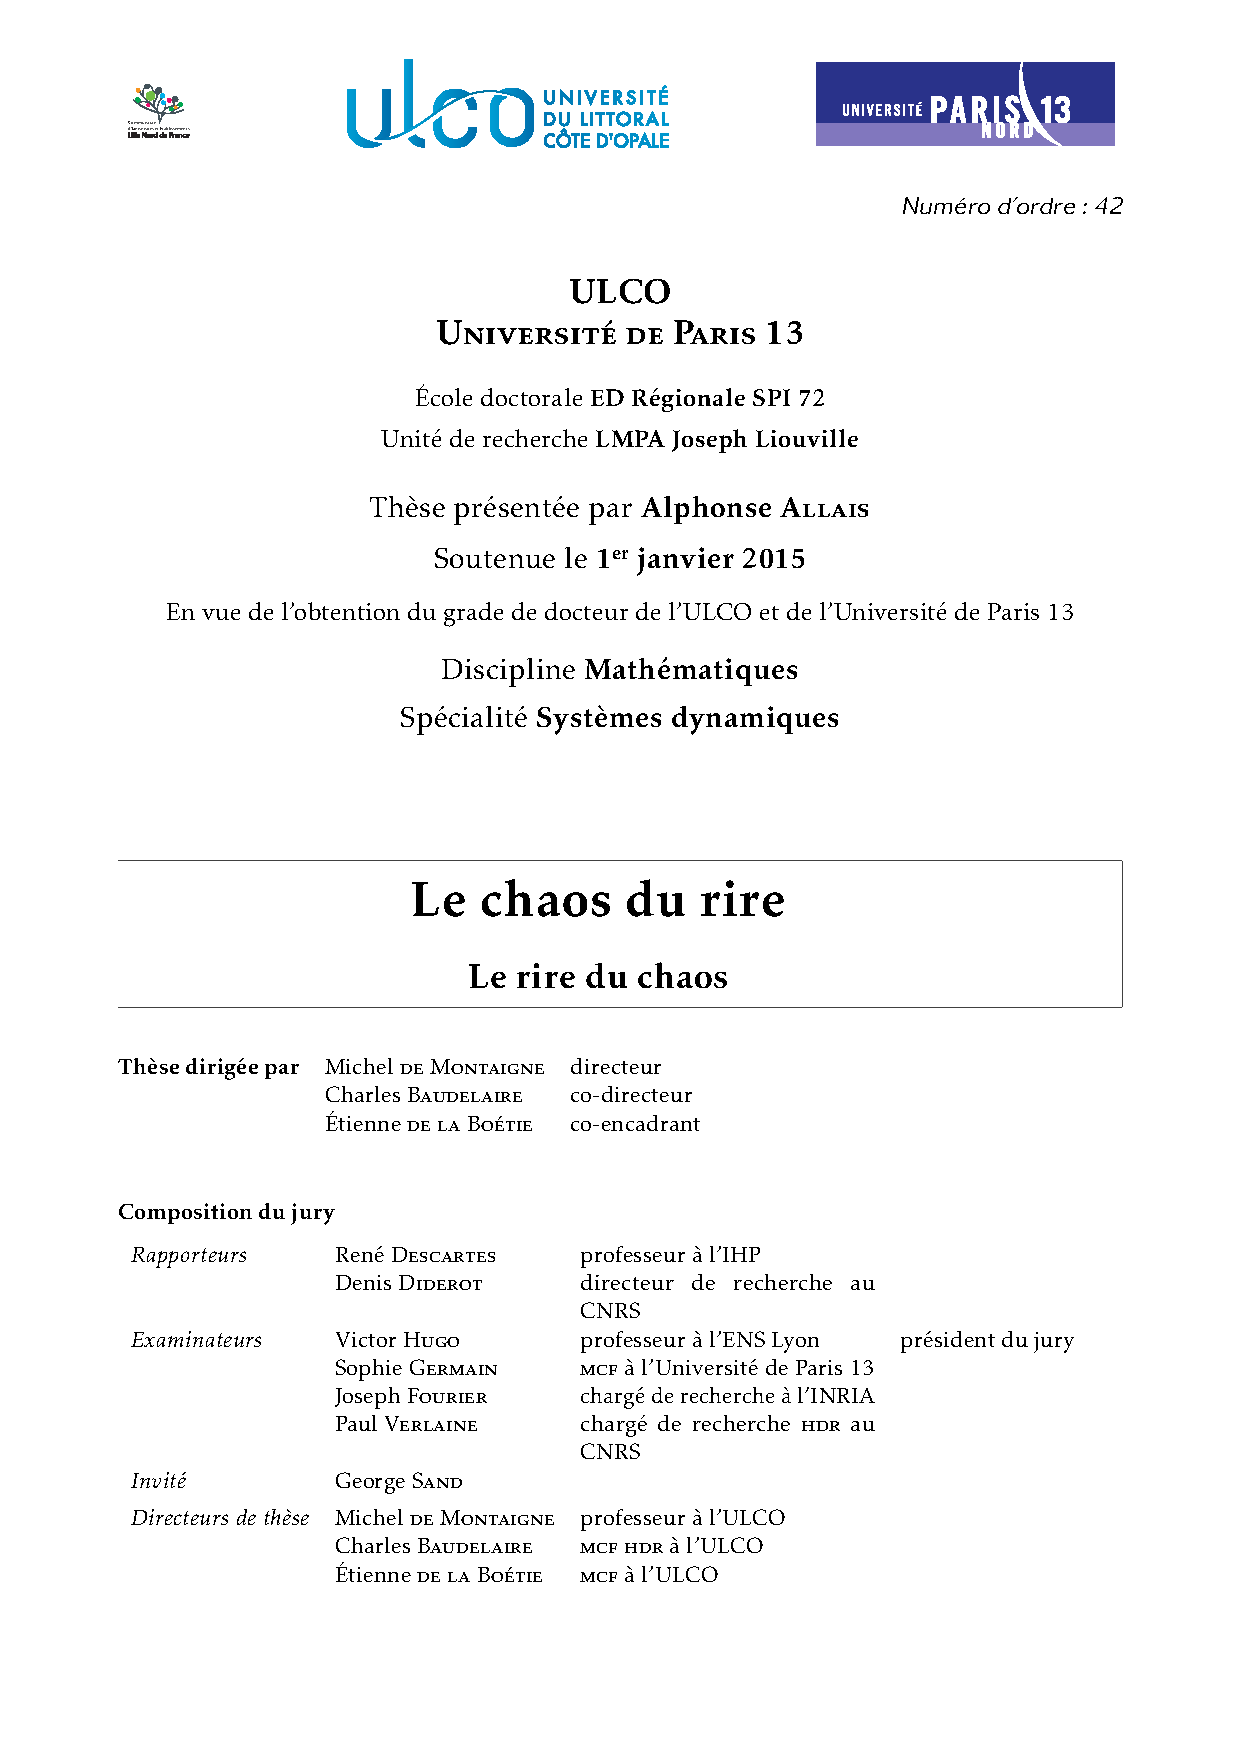
\includegraphics[page=1,width=\linewidth-2\fboxsep-2\fboxrule]{../exemples/specimen/a-plat/these}}
      %\screenshot[1]{fr-title}
      \caption{Page de 1\iere{} de couverture en français}
      \label{fig-maketitle-fr}
    \end{subfigure}%
    \hspace{\stretch{1}}%
    \begin{subfigure}[b]{.45\linewidth}
      \centering%
      \fbox{\includegraphics[page=5,width=\linewidth-2\fboxsep-2\fboxrule]{../exemples/specimen/a-plat/these}}
      %\screenshot[1]{en-title}
      \caption{Page de titre en anglais}
      \label{fig-maketitle-en}
    \end{subfigure}%
    \caption{Pages de 1\iere{} de couverture et de titre}
    \label{fig-maketitle}
  \end{figure}
\end{landscape}

%%% Local Variables:
%%% mode: latex
%%% TeX-master: "../yathesis-fr"
%%% End:

\chapter{Partie liminaire}\label{cha-liminaires}
\index{liminaire}%
\indexsee{préliminaire}{liminaire}%
\index{partie!liminaire}%

La \gls{liminaire} de la thèse comprend :
\begin{enumerate}
\item la page (éventuelle) de clause de non-responsabilité ;
\item la page (éventuelle) des mots clés de la thèse ;
\item la page (éventuelle) du ou des laboratoires où a été préparée la thèse ;
\item la page (éventuelle) des dédicaces ;
\item la page (éventuelle) des épigraphes ;
\item la page de résumés dans les langues principale et secondaire ;
\item les (éventuels) avertissement, remerciements, résumé substantiel en
  français, avant-propos, etc.
\item la ou les listes (éventuelles), commune ou distinctes :
  \begin{itemize}
  \item des sigles et acronymes\footnote{Par commodité, nous ne parlerons plus
      dans la suite que d'acronymes mais ce qui les concernera s'appliquera de
      façon identique aux sigles.} ;
  \item des symboles ;
  \item des termes du glossaire ;
  \end{itemize}
\item le sommaire ou la table des matières ;
\item la liste (éventuelle) des tableaux ;
\item la liste (éventuelle) des figures ;
\item la liste (éventuelle) des listings informatiques.
\end{enumerate}

\begin{dbremark}{Commande \protect\docAuxCommand*{frontmatter} non nécessaire}{nofrontmatter}
  La commande \docAuxCommand{frontmatter} usuelle de la \Class{book}, employée
  habituellement pour entamer la partie liminaire du document, n'est pas
  nécessaire car la \yatCl{} la charge déjà en sous-main. On verra plus loin
  que, au contraire, la commande analogue \refCom{mainmatter} doit être
  explicitement employée pour entamer la partie principale du document (il en
  est de même des commandes \refCom{appendix} et \refCom{backmatter} pour les
  éventuelles parties annexe et finale).
\end{dbremark}

\section{Clause de non-responsabilité}
\label{sec-clause-de-non}%
\index{clause de non-responsabilité}%

\changes{v0.99d}{2014-06-08}{Élision \enquote{automatique} des articles définis
  précédant \meta{institut} et \meta{co-institut} dans la clause de
  non-responsabilité}%
%
La \yatCl{} permet de faire figurer une clause de non-responsabilité, telle
qu'exigée par certains instituts. Celle-ci apparaît sur une page dédiée et
a pour contenu par défaut une phrase semblable à\selonlangue{} :
\begin{displayquote}
  L'\meta{institut} n'entend donner aucune approbation ni improbation aux
  opinions \'emises dans les th\`eses : ces opinions devront \^etre
  consid\'er\'ees comme propres \`a leurs auteurs.
\end{displayquote}
ou :
\begin{foreigndisplayquote}{english}
  The \meta{institut} neither endorse nor censure authors' opinions expressed in
  the theses: these opinions must be considered to be those of their authors.
\end{foreigndisplayquote}
où l'\meta{institut} est celui défini par la commande \refCom{institute}
\aside*{auquel est adjoint l'éventuel institut de cotutelle}.

La page dédiée à la clause de non-responsabilité est produite par la commande
\refCom{makedisclaimer}.

\begin{docCommand}{makedisclaimer}{}
  Cette commande produit une page où figure, seule et centrée
  verticalement, la clause de non-responsabilité.
\end{docCommand}

\begin{docCommand}{makedisclaimer*}{}
  Cette commande a le même effet que la commande
  \refCom{makedisclaimer} sauf que la clause de non-responsabilité est alignée
  sur le haut de la page et non centrée verticalement.
\end{docCommand}

\begin{dbexample}{Production de la page dédiée à la clause de
    non-responsabilité}{}
  \indexex{clause de non-responsabilité}%
  \NoAutoSpacing%
  %
  \bodysample{production-clause}{}{}%
  Le résultat de ce code est illustré \vref{fig-disclaimerpage}.
\end{dbexample}

\begin{figure}[htbp]
  \centering
  \screenshot{disclaimer}%
  \caption{Page de clause de non-responsabilité}
  \label{fig-disclaimerpage}
\end{figure}

\begin{dbwarning}{Élision automatique non robuste}{elision-disclaimer}
  Dans la clause de non-responsabilité, l'article défini précédant
  \meta{institut} est automatiquement élidé selon l'initiale (voyelle ou
  consonne) du mot suivant. Cette élision automatique n'est donc pas robuste :
  elle peut ne pas donner le résultat escompté si \meta{institut} a pour
  initiale :
  \begin{itemize}
  \item une consonne, mais est de genre féminin ;
  \item une voyelle, mais par le truchement d'une commande\commandeacronyme, et
    non pas \enquote{directement}.
  \end{itemize}
\end{dbwarning}

Pour pallier cet inconvénient, et aussi pour permettre de redéfinir la phrase
par défaut si elle ne convient pas, on pourra recourir à la commande
\refCom{disclaimertext}\footnote{Par souci de compatibilité ascendante, la
  commande désormais obsolète \docAuxCommand{disclaimer} est un alias de la commande
  \refCom{disclaimertext}.}.

\begin{docCommand}[doc updated=2020-03-26]{disclaimertext}{\marg{clause}}
  \index{clause de non-responsabilité!modification}%
  \changes{v1.0.0}{2020-03-26}{Commande \protect\docAuxCommand{disclaimer} remplacée
    par (et alias de) la commande \protect\refCom{disclaimertext}}%
    %
    Cette commande, à placer avant \refCom{makedisclaimer}, permet de redéfinir
    le contenu par défaut de la \meta{clause} de non-responsabilité.
\end{docCommand}

\section{Mots clés}\label{sec-mots-cles}

\begin{docCommand}{makekeywords}{}
  \indexdef{mot clé}%
  Cette commande produit une page où figurent, seuls et centrés
  verticalement, les mots clés de la thèse stipulés au moyen de la commande
  \refCom{keywords}.
\end{docCommand}
%
\begin{docCommand}{makekeywords*}{}
  \indexdef{mot clé}%
  Cette commande a le même effet que la commande
  \refCom{makekeywords} sauf que les mots clés sont alignés sur le haut de la
  page et non centrés verticalement.
\end{docCommand}

\begin{dbexample}{Préparation et production de la page dédiée aux mots clés}{}
  \indexex{mot clé}%
  Les codes suivants produisent la page illustrée \vref{fig-makekeywords}.
  \preamblesample{preparation-mots-cles}{%
    deletekeywords={[1]{keywords}},
    deletekeywords={[5]{keywords}}%
  }{title=Préparation}
  %
  \bodysample{production-mots-cles}{}{title=Production}
\end{dbexample}

\begin{figure}[htbp]
  \centering
  \screenshot{keywords}%
  \caption{Page dédiée aux mots clés}
  \label{fig-makekeywords}
\end{figure}

\section{Laboratoire(s)}
\label{sec-laboratoires}

\begin{docCommand}{makelaboratory}{}
  \indexdef{laboratoire}%
  Cette commande produit une page où figure, seul(s) et centré(s)
  verticalement, le ou les laboratoires où a été préparée la thèse, stipulés au
  moyen de la commande \refCom{laboratory} et éventuellement précisés au moyen
  des clés \refKey{logo}, \refKey{logoheight}, \refKey{telephone},
  \refKey{fax}, \refKey{email} et \refKey{nonamelink}.
\end{docCommand}
%
\begin{docCommand}{makelaboratory*}{}
  \index{laboratoire}%
  Cette commande a le même effet que la commande \refCom{makelaboratory} sauf
  que le ou les laboratoires sont alignés sur le haut de la page et non centrés
  verticalement.
\end{docCommand}

\begin{dbexample}{Préparation et production de la page dédiée au(x) laboratoire(s)}{}
  \indexex{laboratoire}%
  Les codes suivants produisent la page illustrée \vref{fig-makelaboratory}.
  \NoAutoSpacing%
  \preamblesample{preparation-laboratoire}{%
    deletekeywords={url},%
    morekeywords={[2]url},%
  }{title=Préparation}
  %
  \bodysample{production-laboratoire}{}{title=Production}
\end{dbexample}

\begin{figure}[htbp]
  \centering
  \screenshot{laboratory}
  \caption{Page dédiée au(x) laboratoire(s)}
  \label{fig-makelaboratory}
\end{figure}

\section{Dédicaces}

\begin{docCommand}{dedication}{\marg{dédicace}}
  \indexdef{dédicace}%
  Cette commande, à employer autant de fois que
  souhaité\hauteurpage{}, permet de préparer une dédicace.
\end{docCommand}

\begin{docCommand}{makededications}{}
  \index{dédicace}%
  Cette commande produit une page où figurent, seules, alignées à droite et
  centrées verticalement, la ou les dédicaces stipulées au moyen de la commande
  \refCom{dedication}.
\end{docCommand}
%
\begin{docCommand}{makededications*}{}
  \index{dédicace}%
  Cette commande a le même effet que la commande \refCom{makededications} sauf
  que la ou les dédicaces sont alignées sur le haut de la page et non centrées
  verticalement.
\end{docCommand}

\begin{dbexample}{Préparation et production de la page dédiée aux dédicaces}{}
  \indexex{dédicace}%
  \NoAutoSpacing%
  \preamblesample{preparation-dedicaces}{}{title=Préparation}
  %
  \bodysample{production-dedicaces}{}{title=Production}
  Le résultat de ce code est illustré \vref{fig-dedicationspage}.
\end{dbexample}

\begin{figure}[htbp]
  \centering
  \screenshot{dedications}%
  \caption{Page de dédicaces}
  \label{fig-dedicationspage}
\end{figure}

\section{Épigraphes liminaires}

\begin{docCommand}{frontepigraph}{\oarg{langue}\marg{épigraphe}\marg{auteur}}
  \indexdef{épigraphe}%
  Cette commande, à employer autant de fois que souhaité\hauteurpage{}, permet
  de préparer une épigraphe destinée à apparaître sur une page dédiée de la
  \gls{liminaire}.

  Si l'épigraphe est exprimée dans une \meta{langue} \aside{connue du
    \Package{babel}} autre que la langue principale du document, on peut le
  spécifier en argument optionnel%
  \footnote{Si cette \meta{langue} est autre que le français ou l'anglais, elle
    doit être explicitement chargée en option de la commande
    \docAuxCommand{documentclass} (cf.  \vref{rq-languessupplementaires}).}.
\end{docCommand}

\begin{docCommand}{makefrontepigraphs}{}
  \index{épigraphe}%
  Cette commande produit une page où figurent, seules, alignées à droite et
  centrées verticalement, la ou les épigraphes stipulées au moyen de la
  commande \refCom{frontepigraph}.
\end{docCommand}
%
\begin{docCommand}{makefrontepigraphs*}{}
  \index{épigraphe}%
  Cette commande a le même effet que la commande \refCom{makefrontepigraphs}
  sauf que la ou les épigraphes sont alignées sur le haut de la page et non
  centrées verticalement.
\end{docCommand}

\begin{dbexample}{Préparation et production de la page dédiée aux épigraphes
    liminaires}{}
  \indexex{épigraphe}%
  \NoAutoSpacing%
  Les codes suivants produisent la page illustrée \vref{fig-epigraphspage}.
  \preamblesample{preparation-epigraphes}{}{title=Préparation}
  %
  \bodysample{production-epigraphes}{}{title=Production}
\end{dbexample}

\begin{figure}[htbp]
  \centering
  \screenshot{frontepigraphs}
  \caption{Page d'épigraphes liminaires}
  \label{fig-epigraphspage}
\end{figure}

\begin{dbremark}{Épigraphes ailleurs dans le document}{}
  Pour gérer les épigraphes liminaires, la \yatCl{} exploite le
  \Package*{epigraph} \aside*{qui est automatiquement chargé}. Il est bien sûr
  possible de recourir aux commandes de ce package pour faire figurer, ailleurs
  dans le mémoire, d'autres épigraphes.
\end{dbremark}

\section{Remerciements, avertissement, résumé substantiel, avant-propos, etc.}
\index{avertissement}%
\index{remerciements}%
\index{résumé}%
\index{avant-propos}%

La \gls{liminaire} d'un mémoire de thèse peut contenir des remerciements, un
avertissement, un résumé substantiel en français (cf. \vref{wa-frenchabstract}),
un avant-propos, etc.  à considérer et à composer comme des chapitres
\enquote{ordinaires}.

\begin{dbwarning}{Chapitres \enquote{ordinaires} de la \gls{liminaire}
    automatiquement \emph{non} numérotés}{}
  \index{chapitre!non numéroté}%
  Les chapitres \enquote{ordinaires} de la \gls{liminaire} doivent être
  introduits au moyen de la commande usuelle \docAuxCommand{chapter}, sous sa
  forme \emph{non} étoilée : puisqu'ils seront situés dans la partie liminaire
  du mémoire, ces chapitres seront automatiquement \emph{non} numérotés.
\end{dbwarning}

%\begin{dbremark}{\protect\Glspl{titrecourant} des chapitres de la
%  \protect\gls{liminaire}}{titrecourant}%
%  Les chapitres \enquote{ordinaires} sont pourvus de \glspl{titrecourant}
%  si (et seulement si) ils figurent après la page dédiée aux résumés
%  (cf. \vref{sec-abstract}).
%\end{dbremark}

\section{Résumés succincts en français et en anglais}\label{sec-abstract}

Une page contenant de courts résumés en français et en anglais est requise.
L'environnement \refEnv{abstract} suivant permet de préparer une telle
page.
%
\begin{docEnvironment}[doclang/environment content=résumé,doc description=\mandatory]{abstract}{\oarg{titre alternatif}}
  \indexdef{résumé}%
  \index{résumé!en français}%
  \index{résumé!en anglais}%
  Cet environnement, destiné à recevoir le ou les \meta{résumé}s de la thèse, est
  conçu pour être employé une ou deux fois :
  \begin{enumerate}
  \item sa 1\iere{} occurrence doit contenir le \meta{résumé} dans la langue
    principale ;
  \item sa 2\ieme{} occurrence, si présente, doit contenir le \meta{résumé} dans la
    langue secondaire.
  \end{enumerate}
  Ces \meta{résumé}s figurent, dans les langues principale et secondaire :
  \begin{itemize}
  \item sur la page dédiée au(x) résumé(s) de la thèse produite par la commande
    \refCom{makeabstract} ;
  \item sur la 4\ieme{} de couverture si la commande \refCom{makebackcover} est
    employée.
  \end{itemize}
  Ils \index{nom!résumé}%
  sont respectivement intitulés \enquote{\abstractname} ou
  \enquote{\selectlanguage{english}\abstractname}\selonlangueshort{} mais
  l'argument optionnel permet de spécifier un \meta{titre} (ou \meta{nom})
    \meta{alternatif}\redefexprcle.
\end{docEnvironment}

\begin{docCommand}[doc description=\mandatory]{makeabstract}{}
  \index{résumé}%
  Cette commande produit une page dédiée aux résumés en y faisant
  apparaître automatiquement :
  \begin{enumerate}
  \item dans les langues principale et secondaire :
    \begin{itemize}
    \item les titre, éventuel sous-titre et mots clés de la thèse, stipulés au
      moyen des commandes respectives \refCom{title}, \refCom{subtitle} et
      \refCom{keywords} ;
    \item les résumés saisis au moyen de l'environnement \refEnv{abstract} ;
    \end{itemize}
  \item le nom et l'adresse du laboratoire (principal)\footnote{Il est possible
      de faire figurer sur les pages de résumés et de 4\ieme{} de couverture un
      nombre arbitraire de laboratoires au moyen de la clé
      \refKey{numlaboratories}.} dans lequel la thèse a été préparée, stipulés
    au moyen de la commande \refCom{laboratory}.
  \end{enumerate}
\end{docCommand}

\begin{dbexample}{Préparation et production de la page dédiée aux résumés}{}
  \indexex{résumé}%
  Les codes suivants produisent la page illustrée \vref{fig-resumes-succincts}.
  \preamblesample{preparation-resumes}{}{title=Préparation des résumés}
  \bodysample{production-resumes}{}{title=Production des résumés}
  %
\end{dbexample}

\begin{figure}[htbp]
  \centering
  \screenshot{abstract}%
  \caption{Page de résumés succincts en français et en anglais}
  \label{fig-resumes-succincts}
\end{figure}

\begin{dbwarning}{Résumés nécessairement courts dans l'environnement
    \protect\lstinline+abstract+}{}
  L'environnement \refEnv{abstract} est prévu pour des résumés courts, leurs
  versions dans les langues principale et secondaire devant tenir l'une sous
  l'autre sur une seule et même page. Cette limitation est en phase avec les
  recommandations du ministère stipulant que ces résumés doivent chacun
  contenir au maximum 1700~caractères, espaces compris\footnote{En cas de
    débordement sur plus d'une page, on pourra toujours recourir à un
    changement local de taille des caractères.}.
\end{dbwarning}

\begin{dbwarning}{Résumé en français nécessaire en cas de mémoire en langue
    étrangère}{frenchabstract}
  Un mémoire composé principalement en langue étrangère \aside{notamment dans
    le cadre d'une cotutelle internationale} requiert, en sus de la page de
  résumé(s) ci-dessus, un résumé \emph{en français} de la thèse. Celui-ci doit
  être \emph{substantiel}, d'une dizaine de pages environ.
\end{dbwarning}

\section{Liste d'acronymes, liste de symboles,
  glossaire}\label{sec-sigl-gloss-nomencl}
\index{acronyme!liste d'---s}%
\index{symbole!liste de ---s}%
\index{glossaire}%

\begin{dbremark*}{Section à passer en 1\iere{} lecture}
  Cette section est à passer en 1\iere{} lecture si on ne compte faire figurer
  ni listes d'acronymes, ni listes de symboles, ni glossaire.
\end{dbremark*}

Tout système de gestion de glossaire peut théoriquement être mis en œuvre avec
la \yatCl. Cependant, celle-ci fournit des fonctionnalités propres au
\Package{glossaries}\footnote{Dans ses versions à partir de la \texttt{4.0} en
  date du \formatdate{14}{11}{2013}. Dans cette section, le fonctionnement de
  ce package est supposé connu du lecteur (sinon, cf. par exemple
  \cite{en-ligne7}).} :
\begin{itemize}
\item une commande \refCom{newglssymbol}, destinée à faciliter la définition de
  symboles dans la base terminologique ;
\item un style de glossaire \docValue{yadsymbolstyle}, destiné à composer la
  liste des symboles sous forme de \enquote{nomenclature} (dans l'esprit du
  \Package*{nomencl}).
\end{itemize}

\begin{dbwarning}{Package \package{glossaries} non chargé par défaut}{}
  Le \Package{glossaries} \emph{n'étant pas} chargé par la \yatCl, on veillera
  à le charger manuellement si on souhaite l'utiliser.
\end{dbwarning}

% \begin{enumerate}
% \item les commandes de ce package produisant les liste des termes du ou des
%   glossaires sont légèrement modifiées (un style de pages propre leur étant
%   appliqué) :
%   \begin{itemize}
%   \item \docAuxCommand{printglossary} et \docAuxCommand{printglossaries} qui
%     produisent la liste des termes du ou des glossaires\termesdefinisutilises{}
%     (cf. \vref{fig-printglossary}) ;
%   \item \docAuxCommand{printacronyms}\footnote{L'usage de la commande
%       \docAuxCommand{printacronyms} nécessite que l'option \docAuxKey{acronyms}
%       soit passée au \Package{glossaries}.} qui produit la liste des
%     acronymes\termesdefinisutilises{} (cf. \vref{fig-printacronyms}) ;
%   \end{itemize}
% \item les commande et style propres \refCom{newglssymbol}, et
%   \docValue{yadsymbolstyle}, précisés ci-dessous, sont définis.
% \end{enumerate}

\begin{docCommand}{newglssymbol}{\oarg{classement}\marg{label}\marg{symbole}\marg{nom}\marg{description}}
  \indexdef{symbole}%
  Cette commande définit un symbole au moyen :
  \begin{itemize}
  \item de son \meta{label}\footnote{Ce \meta{label}, qui identifie le symbole de
      manière unique dans la base terminologique, est notamment utilisé dans
      les commandes qui produisent celui-ci dans le texte \aside*{par exemple
      \docAuxCommand{gls}\marg{label}}.} ;
\item du \meta{symbole} proprement dit\footnote{Ce symbole peut notamment être
    composé au moyen de la commande \docAuxCommand{ensuremath}\marg{symbole
      mathématique} ou de la commande \docAuxCommand{si}\marg{commande d'unité}
    du \Package*{siunitx} (à charger).} ;
  \item de son \meta{nom} ;
  \item de sa \meta{description}.
  \end{itemize}
  Dans la liste des symboles produite par la commande \refCom{printsymbols}, un
  symbole est par défaut classé selon l'ordre alphabétique de son \meta{label}
  mais peut optionnellement l'être selon celui d'une autre chaîne de
  \meta{classement}.
\end{docCommand}

\begin{dbwarning}{Option \texttt{symbols} nécessitée par la commande
    \protect\refCom*{newglssymbol}}{}
  L'usage de la commande \refCom{newglssymbol} nécessite que l'option
  \docAuxKey{symbols} soit passée au \Package{glossaries}.
\end{dbwarning}

\begin{docCommand}{printsymbols}{\oarg{options}}
  \index{symbole!liste de ---s}%
  Cette commande, fournie par le \Package{glossaries}, produit la liste des
  symboles saisis au moyen de (par exemple) la commande
  \refCom{newglssymbol}. Mais elle a été légèrement redéfinie, sa clé
  \refKey{style} ayant pour valeur par défaut \docValue{yadsymbolstyle} (et non
  \docValue{list}) :
  \begin{docKey}{style}{=\docValue{yadsymbolstyle}\textbar\meta{style}}{pas de valeur
      par défaut, initialement \docValue{yadsymbolstyle}}
    Cette clé permet de spécifier le style appliqué à la liste des
    symboles. Tout \meta{style} spécifié, autre que \docValue{yadsymbolstyle},
    doit être l'un de ceux acceptés par la clé \refKey{style} du
    \Package{glossaries}.
  \end{docKey}
\end{docCommand}

\begin{dbexample}{Définitions et liste des symboles}{}
  \indexex{symbole}%
  Le code suivant définit certains symboles.
  \preamblesample{preparation-symboles}{}{title=Préparation}%
  Le code suivant produit la liste de ces symboles \aside*{composée avec le
    style \docValue{yadsymbolstyle}}.
  \bodysample{production-symboles}{}{title=Production}%
  Le résultat de ce code est illustré \vref{fig-printsymbols}.
\end{dbexample}

% \afterpage{%
\begin{landscape}
  \begin{figure}[p]
    \centering
    \begin{subfigure}[b]{.45\linewidth}
      \centering
      \screenshot[1]{printacronyms}
      \caption{Acronymes}
      \label{fig-printacronyms}
    \end{subfigure}%
    \hspace{\stretch{1}}%
    \begin{subfigure}[b]{.45\linewidth}
      \centering
      \screenshot[1]{printsymbols}
      \caption{Symboles}
      \label{fig-printsymbols}
    \end{subfigure}%
    \caption{Listes des acronymes et des symboles}
    \label{fig-printacronyms-printsymbols}
  \end{figure}
\end{landscape}
% }

% Si on souhaite faire figurer :
% \begin{enumerate}
% \item une liste \emph{commune} des acronymes et des termes du glossaire, on
%   chargera \package{glossaries} \emph{sans} l'option |acronym| et on recourra à
%   la commande \docAuxCommand{printglossary} ;
% \item deux listes \emph{distinctes}, on chargera \package{glossaries}
%   \emph{avec} l'option |acronym|. et on recourra à la commande
%   \begin{enumerate}
%   \item \refCom{printacronyms} pour celle des acronymes (cf.
%     \vref{fig-acronymes}) ;
%   \item\label{item:1} \docAuxCommand{printglossary} pour celle des termes du
%     glossaire (cf. \vref{fig-printglossary}).
%   \end{enumerate}
% \end{enumerate}

Dans un mémoire de thèse, les emplacements des listes des termes du glossaire,
des acronymes\footnote{Les commandes \docAuxCommand{printglossary} et
  \docAuxCommand{printacronyms} du \Package{glossaries}, produisant les listes
  des termes du glossaire et des acronymes, sont illustrées
  \vref{fig-printglossary,fig-printacronyms}.} et des symboles sont \emph{a
  priori} arbitraires. Il est cependant parfois conseillé de placer :
\begin{itemize}
\item si elles sont \emph{communes}, \emph{la} liste résultante en partie finale ;
\item si elles sont \emph{distinctes} :
  \begin{enumerate}
  \item les listes des acronymes et des symboles avant qu'ils soient utilisés
    pour la première fois donc, \emph{a priori}, avant le ou les résumés ;
  \item la liste des termes du glossaire en partie finale.
  \end{enumerate}
\end{itemize}

\section{Sommaire et/ou table des matières}\label{sec-table-des-matieres}

La \yatCl{} redéfinit la commande \refCom{tableofcontents} habituelle de
création des tables des matières \enquote{globales}\footnote{Par opposition aux
  tables des matières locales\index{table des matières!locale},
  cf. \vref{sec-localtoc}.} pour permettre de facilement
\begin{itemize}
\item l'utiliser plusieurs fois dans le mémoire ;
\item en spécifier la profondeur ;
\item en modifier le nom.
\end{itemize}

\begin{docCommand}[doc description=\mandatory]{tableofcontents}{\oarg{options}}
  \indexdef{table des matières}%
  Cette commande produit une table des matières dont le \enquote{niveau de
    profondeur} par défaut est celui des sous-sections : les intitulés des
  commandes de structuration qui y figurent sont (seulement) ceux des parties
  (éventuelles), des chapitres, des sections et des sous-sections.
\end{docCommand}

L'argument optionnel de la commande \refCom{tableofcontents} permet de stipuler
des \meta{options} sous la forme d'une liste \meta{clé}|=|\meta{valeur} dont
les clés disponibles sont les deux suivantes.
  %
{%
  \tcbset{before lower=\vspace*{.5\baselineskip}\par}
    %
  \begin{docKey}{depth}{=\docValue{part}\textbar\docValue{chapter}\textbar\docValue{section}\textbar\docValue{subsection}\textbar\docValue{subsubsection}\textbar\docValue{paragraph}\textbar\docValue{subparagraph}}{pas
      de valeur par défaut, initialement \docValue{subsection}}
    \index{table des matières!globale!profondeur}%
    \index{profondeur!table des matières!globale}%
    Cette clé permet de modifier le \enquote{niveau de profondeur} de la table
    des matières, respectivement jusqu'aux : parties, chapitres, sections,
    sous-sections, sous-sous-sections, paragraphes, sous-paragraphes.
  \end{docKey}
}
%
\begin{docKey}{name}{=\meta{nom alternatif}}{pas de valeur par défaut,
    initialement \docAuxCommand{contentsname}}
  \index{table des matières!globale!nom}%
  \index{table des matières!globale!titre}%
  \index{nom!de la table des matières}%
  \index{titre!de la table des matières}%
  Par défaut, le nom de la table des matières est \docAuxCommand{contentsname},
  c'est-à-dire \enquote{\contentsname} ou
  \enquote{\selectlanguage{english}\contentsname}\selonlangueshort{}. Cette clé
  permet de spécifier un \meta{nom alternatif}\redefexprcle.
\end{docKey}

\begin{dbremark}{Tables des matières multiples}{}
  \index{table des matières!globale!multiple}%
  Si la table des matières est longue, il est conseillé de la placer en fin de
  document mais de faire alors figurer, en \gls{liminaire}, un sommaire
  c'est-à-dire par une table des matières allégée.

  À cet effet, la \yatCl{} permet de faire figurer, dans un même document,
  plusieurs tables des matières au moyen d'occurrences multiples de la commande
  \refCom{tableofcontents}, chacune d'elles étant sujette aux options
  précédentes.
\end{dbremark}

\begin{dbexample}{Sommaire et table des matières}{sommaire-table-des-matieres}
  \indexex{table des matières}%
  Pour faire figurer, dans un même document :
  \begin{enumerate}
  \item un sommaire :
    \begin{itemize}
    \item ne faisant apparaître que les chapitres (et éventuelles parties) ;
    \item nommé \enquote{Sommaire} ;
    \end{itemize}
  \item la table des matières ;
  \end{enumerate}
  on insérera respectivement :
  %
  \bodysample{sommaire}{}{}
  %
  et :
  %
  \bodysample{table-des-matieres}{}{}
  %
  La \vref{fig-tableofcontentsto-tableofcontents} illustre ce code.
\end{dbexample}

\afterpage{%
  \begin{landscape}
    \begin{figure}[p]
      \centering
      \begin{subfigure}[b]{.45\linewidth}
        \centering%
        \screenshot[1]{tableofcontents-withargument}
        \caption{Sommaire allant jusqu'aux chapitres}
        \label{fig-tableofcontentsto}
      \end{subfigure}%
      \hspace{\stretch{1}}%
      \begin{subfigure}[b]{.45\linewidth}
        \centering%
        \screenshot[1]{tableofcontents-withoutargument}
        \caption{Table des matières allant jusqu'aux sous-sections}
        \label{fig-tableofcontents}
      \end{subfigure}%
      \caption[Sommaire et table des matières]{Sommaire et table des matières
        de profondeurs différentes dans un même document}
      \label{fig-tableofcontentsto-tableofcontents}
    \end{figure}
  \end{landscape}
}

\section{Tables et listes usuelles}
\index{figure!table des ---s}%
\index{table des figures}%
\index{liste des tableaux}%
\indexsee{table des tableaux}{liste des tableaux}%
\index{tableau!liste des ---x}%
\index{table des listings}%
\index{listing informatique!table des ---s}%

Les commandes usuelles |\listoftables| et |\listoffigures| produisent les
listes respectivement des tableaux et des figures.
%
On peut faire figurer d'autres listes, par exemple celle des listings
informatiques au moyen de la commande |\lstlistoflistings| du
\Package*{listings}.
%
Nous n'illustrons pas ces commandes, classiques.

%%% Local Variables:
%%% mode: latex
%%% TeX-master: "../yathesis-fr"
%%% End:

\chapter{Partie principale}\label{cha-corps}
\index{partie!principale}%

La partie principale de la thèse, qu'on appelle aussi son \enquote{corps},
comprend :
\begin{enumerate}
\item\index{introduction}%
 l'introduction (\enquote{générale}) ;
\item\index{chapitre!ordinaire}%
  les chapitres \enquote{ordinaires} ;
\item\index{conclusion}%
  la conclusion (\enquote{générale}) ;
\item\index{bibliographie!globale}%
  la bibliographie.
\end{enumerate}
Les introduction et conclusion peuvent éventuellement être
\enquote{générales} par exemple si la thèse comporte plusieurs
parties, chacune introduite par une introduction et conclue par
une conclusion \enquote{ordinaires}.

\begin{dbremark}{Scission du mémoire en fichiers maître et esclaves}{}
  \index{fichier!maître}%
  \index{fichier!esclave}%
  Il est vivement recommandé de scinder le mémoire de thèse,
  notamment son corps, en fichiers maître et esclaves (ces derniers
  correspondants chacun à un chapitre). La procédure
  pour ce faire, standard, est rappelée \vref{sec-repart-du-memo}.
\end{dbremark}

\section{Initialisation de la partie principale}

\begin{docCommand}[doc description=\mandatory]{mainmatter}{}
  La partie principale de la thèse doit être manuellement introduite au moyen
  de la commande usuelle \docAuxCommand{mainmatter}\nofrontmatter.
\end{docCommand}

\section{Commandes de structuration}

La \yatCl{} modifie les commandes usuelles de structuration
(\docAuxCommand{chapter}, \docAuxCommand{section}, \docAuxCommand{subsection},
etc.)  en ce qui concerne les trois aspects suivants (examinés aux
\vref{sec-chap-non-numer,sec-intit-altern,sec-chapitres-numerotes}) :
\begin{description}
\item[titres alternatifs des chapitres et sections :] il est possible de
  différencier celui figurant en \gls{tdm} de celui figurant en
  entête (c'est-à-dire en \gls{titrecourant}) ;
\item[unités \emph{non} numérotées :] l'usage des variantes étoilées des
  commandes de structuration est simplifié ;
\item[têtes de chapitres numérotés :] leur mise en forme est modifiée (et
  modifiable).
\end{description}

\subsection{Titres alternatifs des chapitres et sections}
\label{sec-intit-altern}
\index{table des matières!entrée différente du titre courant}%
\index{titre courant!différent de l'entrée en table des matières}%
\index{titre!d'unité!alternatif}
\index{titre!d'unité!normal}

\changes{v0.99p}{2016-12-08}{Commandes \protect\refCom{chapter} et
  \protect\refCom{section} pourvues d'un argument optionnel supplémentaire
  permettant de stipuler un titre alternatif en entête différent de celui
  en \gls{tdm}}%

Avec la \yatCl{}, les entêtes de la plupart des pages contiennent le titre du
chapitre et le titre de l'éventuelle section en cours
(cf. \vref{cha-pagination}).
%
Ce titre est par défaut celui stipulé en argument obligatoire des commandes
respectivement \docAuxCommand{chapter} et \docAuxCommand{section}, et figure
alors également dans le fil du texte et en \gls{tdm}\signet{}.

% Les commandes \docAuxCommand{chapter} et \docAuxCommand{section} admettent un
% argument obligatoire permettant de stipuler le \meta{titre} du chapitre et de la
% section dans le fil du texte, \meta{titre} qui par défaut figure également en
% \gls{tdm}\signet{} et en entête.
%
Les classes standard offrent la possibilité de faire figurer en
\gls{tdm}\signet{} et en entête \emph{un} titre alternatif, différent de celui
stipulé en argument obligatoire : il suffit pour cela de recourir
à l'\emph{unique} argument optionnel des commandes \docAuxCommand{chapter} et
\docAuxCommand{section}. Mais ce titre alternatif est alors nécessairement
\emph{identique} en \gls{tdm}\signet{} et en entête.

La \yatCl{} fournit une fonctionnalité supplémentaire : grâce aux \emph{deux}
arguments optionnels dont elle dote les commandes \docAuxCommand{chapter} et
\docAuxCommand{section}, le titre alternatif en entête peut être différencié de
celui en \gls{tdm}\signet{}.

La nouvelle syntaxe indiquée ci-dessous, commune aux commandes \refCom{chapter}
et \refCom{section},
% n'est indiquée ci-dessous que pour \refCom{chapter} mais
est précisée et synthétisée au \vref{tab-commande-chapter-section}.

\begin{docCommand}[doc new=2016-12-08]{chapter}{\oarg{alt. en {\normalfont\ttfamily\glsxtrshort*{tdm}}}\oarg{alt. en entête}\marg{titre}}
  \indexdef{chapitre!titre alternatif}%
  % Cette commande crée un chapitre dont le titre :
  % \begin{itemize}
  % \item dans le fil du texte est \meta{titre} ;
  % \item alternatif en \gls{tdm}\signet{} est \meta{alt. en {\normalfont\ttfamily\glsxtrshort*{tdm}}} ;
  % \item alternatif en entête est \meta{alt. en entête}.
  % \end{itemize}
\end{docCommand}
%
\begin{docCommand}[doc new=2016-12-08]{section}{\oarg{alt. en {\normalfont\ttfamily\glsxtrshort*{tdm}}}\oarg{alt. en entête}\marg{titre}}
  \indexdef{section!titre alternatif}%
  Ces commandes créent respectivement un chapitre et une section dont le titre :
  \begin{itemize}
  \item dans le fil du texte est \meta{titre} ;
  \item alternatif en \gls{tdm}\signet{} est \meta{alt. en {\normalfont\ttfamily\glsxtrshort*{tdm}}} ;
  \item alternatif en entête est \meta{alt. en entête}.
  \end{itemize}
  % Son usage précis est synthétisé au \vref{tab-commande-chapter-section}.
\end{docCommand}
%
\begin{table}[htb]
  \centering
  \caption{Usage des (deux arguments optionnels des) commandes
    \protect\refCom{chapter} et \protect\refCom{section}%  (identique pour les
    % commandes \docAuxCommand{chapter*} et \docAuxCommand{section*})
  }
  \label{tab-commande-chapter-section}
  \footnotesize%
\lstset{%
  deletekeywords={chapter},deletekeywords={[3]chapter},%
  deletekeywords={section},deletekeywords={[3]section},%
}
\begin{tabular}{|l|c|c|c|}
  \cline{2-4}
  \multicolumn{1}{c|}{}
                                                                                                                                                      &
    fil
    du texte                                                                                                                                          & \gls{tdm}
                                                                                                                                                      & entête                                                                                                                                                           \\\hline
  \lstinline+\chapter{+\meta{titre}\lstinline+}+                                                                                                      & \multicolumn{3}{c|}{}                                                                                                                                            \\
  \lstinline+\section{+\meta{titre}\lstinline+}+                                                                                                      & \multicolumn{3}{c|}{\multirow{-2}*{\meta{titre}}}                                                                                                                \\\hline
  \lstinline+\chapter[+\meta{alt. en {\normalfont\ttfamily\glsxtrshort*{tdm}}}\lstinline+]{+\meta{titre}\lstinline+}+                                    &                                                   & \multicolumn{2}{c|}{}                                                                                        \\
  \lstinline+\section[+\meta{alt. en {\normalfont\ttfamily\glsxtrshort*{tdm}}}\lstinline+]{+\meta{titre}\lstinline+}+                                    & \multirow{-2}*{\meta{titre}}                      & \multicolumn{2}{c|}{\multirow{-2}*{\meta{alt. en {\normalfont\ttfamily\glsxtrshort*{tdm}}}}}                    \\\hline
  \lstinline+\chapter[][+\meta{alt. en entête}\lstinline+]{+\meta{titre}\lstinline+}+                                                                 & \multicolumn{2}{c|}{}                             &                                                                                                              \\
  \lstinline+\section[][+\meta{alt. en entête}\lstinline+]{+\meta{titre}\lstinline+}+                                                                 & \multicolumn{2}{c|}{\multirow{-2}*{\meta{titre}}} & \multirow{-2}*{\meta{alt. en entête}}                                                                        \\\hline
  \lstinline+\chapter[+\meta{alt. en {\normalfont\ttfamily\glsxtrshort*{tdm}}}\lstinline+][+\meta{alt. en entête}\lstinline+]{+\meta{titre}\lstinline+}+ &                                                   &                                                                      &                                       \\
  \lstinline+\section[+\meta{alt. en {\normalfont\ttfamily\glsxtrshort*{tdm}}}\lstinline+][+\meta{alt. en entête}\lstinline+]{+\meta{titre}\lstinline+}+ & \multirow{-2}*{\meta{titre}}                      & \multirow{-2}*{\meta{alt. en {\normalfont\ttfamily\glsxtrshort*{tdm}}}} & \multirow{-2}*{\meta{alt. en entête}} \\\hline
\end{tabular}

%%% Local Variables:
%%% mode: latex
%%% TeX-master: "../yathesis-fr"
%%% End:

\end{table}
%
\begin{dbremark}{Titres alternatifs différenciables aussi pour
    \protect\docAuxCommand*{chapter*} et \protect\docAuxCommand*{section*}%  les chapitres et
    % sections non numérotés
  }{}
  Les commandes \docAuxCommand{chapter*} et \docAuxCommand{section*}, permettant
  de créer des chapitres et sections non numérotés, partagent la syntaxe des
  commandes \docAuxCommand{chapter} et \docAuxCommand{section} synthétisée au
  \vref{tab-commande-chapter-section} : elles admettent donc elles aussi deux
  arguments optionnels permettant de différencier les titres alternatifs
  en \gls{tdm}\signet{} et en entête.
\end{dbremark}
%
La syntaxe des commandes \docAuxCommand{subsection},
\docAuxCommand{subsubsection}, \docAuxCommand{paragraph} et
\docAuxCommand{subparagraph} n'est pas modifiée par rapport à celle de la
\Class{book} ; en effet, les titres correspondants ne figurant que dans le fil
du texte et (éventuellement) en \gls{tdm}\signet{}, il est inutile de pouvoir en
stipuler une version spécifique aux entêtes.
%
\subsection{Unités du mémoire non numérotées}
\label{sec-chap-non-numer}%
% \indexdef{chapitre!non numéroté}%
\indexdef{unité!du mémoire!non numérotée}%
% \indexsee{numérotation!unité}{unité!du mémoire!non numérotée}%

\changes{v0.99p}{2016-12-08}{%
  Simplification de l'usage de toutes les commandes de structuration étoilées
  (et plus seulement de \protect\docAuxCommand{chapter*})%
}

Si certaines unités du corps de la thèse \aside{par exemple des chapitres
  d'introduction et de conclusion \enquote{générales}} doivent être \emph{non}
numérotées, on recourra de façon usuelle à la version étoilée des commandes
correspondantes. Ces dernières ont toutefois été quelque peu modifiées afin d'en
simplifier l'usage.

%  : habituellement, si un chapitre non numéroté est créé
% \emph{dans la partie principale} (entre \docAuxCommand{mainmatter} et
% \docAuxCommand{backmatter}) avec la commande standard
% \docAuxCommand{chapter*} :
% \begin{enumerate}
% \item des précautions (assez techniques) doivent être prises pour que :
%   \begin{enumerate}
%   \item le titre correspondant figure dans la table des matières ;
%   \item les entêtes correspondants soient corrects ;
%   \end{enumerate}
% \item toutes les (sous-(sous-))sections du chapitre, nécessairement non
%   numérotées elles aussi, doivent également être créées avec les versions
%   étoilées des commandes correspondantes : \docAuxCommand{section*},
%   \docAuxCommand{subsection*} et \docAuxCommand{subsubsection*}.
% \end{enumerate}

\begin{dbremark}{Variantes étoilées des commandes de structuration modifiées}{}
  La \yatCl{} modifie les variantes étoilées des commandes de structuration
  (\docAuxCommand{chapter*}, \docAuxCommand{section*},
  \docAuxCommand{subsection*}, etc.) de sorte que :
  \begin{enumerate}
  \item automatiquement, le titre (alternatif le cas échéant) correspondant
    figure :
    \begin{enumerate}
    \item en \gls{tdm} (selon la profondeur choisie : cf. \refKey{depth} et
      \refKey{localtocs/depth}) ;
    \item en entête (pour les chapitres et sections seulement) ;
    \end{enumerate}
  \item si les unités correspondantes contiennent des sous-unités, ces dernières
    puissent (et même \emph{doivent}) être créées avec les versions \emph{non}
    étoilées des commandes correspondantes : elles seront néanmoins \emph{non}
    numérotées (comme l'unité les contenant).

    Ainsi, si un chapitre est non numéroté, les sections, sous-sections,
    sous-sous-sections, etc. qu'il contient doivent aussi être non
    numérotées. Et, avec la \yatCl{}, elles seront cependant introduites par les
    commandes \emph{non} étoilées correspondantes : \docAuxCommand{section},
    \docAuxCommand{subsection}, \docAuxCommand{subsubsection}, etc.
  \end{enumerate}
\end{dbremark}

\begin{dbexample}{Introduction}{}
  \indexex{chapitre!non numéroté}%
  \indexex{unité!du mémoire!non numérotée}%
  Le code suivant produit la \vref{fig-introduction} illustrant une introduction
  (générale) non numérotée\footnote{Et, au passage, une table des matières
    locale. Plus de détails \vref{sec-localtoc}.}. On constate que, bien que
  seule la commande \docAuxCommand{chapter} figure sous sa forme étoilée, aucun
  élément de structuration de ce chapitre n'est numéroté.
  %
  \bodysample{introduction}{%
    deletekeywords={[1]introduction},%
    deletekeywords={[3]section,subsection,subsubsection,paragraph,subparagraph}%
  }{}
\end{dbexample}

\begin{figure}[p]
  \centering
  \screenshot{introduction}
  \caption{Introduction (non numérotée)}
  \label{fig-introduction}
\end{figure}

\subsection{Têtes des chapitres numérotés}
\label{sec-chapitres-numerotes}%
\indexdef{chapitre!numéroté}%

Les chapitres numérotés de la thèse, introduits par la version non étoilée de la
commande \docAuxCommand{chapter}, voient leurs têtes composées par défaut avec
le style |PetersLenny| du \Package{fncychap} (cf. \vref{fig-chapitre}). La
\vref{sec-style-des-tetes} explique comment ceci peut être modifié.

\begin{figure}[ht]
  \centering
  \screenshot{chapter}
  \caption[Chapitre \enquote{ordinaire}]{(Première) Page de chapitre
    \enquote{ordinaire}}
  \label{fig-chapitre}
\end{figure}

\section{Références bibliographiques}\label{sec-refer-bibl}
\indexdef{bibliographie!globale}%

Les références bibliographiques font partie intégrante du corps de la thèse.

Tout système de gestion de bibliographie peut théoriquement être mis en œuvre
avec la \yatCl. Cependant, celle-ci a été conçue plus spécifiquement en vue
d'un usage du \Package{biblatex} et éventuellement de \package{biber},
remplaçant fortement conseillé de \hologo{BibTeX}\footnote{Dans cette section,
  leur fonctionnement est supposé connu du lecteur (sinon, cf. par exemple
  \cite{en-ligne6}).}.

\begin{docCommand}[doc description=\mandatory]{printbibliography}{\oarg{options}}
  Cette commande, fournie par \package{biblatex}, produit la liste des
  références bibliographiques saisies selon la syntaxe de ce package (cf.
  \vref{fig-printbibliography}). Mais elle a été légèrement redéfinie de sorte
  que la bibliographie figure automatiquement dans les sommaire, table des
  matières et signets du document.
\end{docCommand}

\begin{figure}[htbp]
  \indexex{bibliographie!globale}%
  \centering
  \screenshot{printbibliography}
  \caption[Bibliographie]{Bibliographie (ici composée avec le style
    bibliographique par défaut)}
  \label{fig-printbibliography}
\end{figure}

\begin{dbwarning}{Package \package{biblatex} non chargé par défaut}{}
  Le \Package{biblatex} \emph{n'étant pas} chargé par la \yatCl, on veillera
  à le charger manuellement si on souhaite l'utiliser, notamment si on souhaite
  bénéficier de l'ajout automatique de bibliographies locales en fin de
  chapitres (cf. \vref{sec-localbibs}).
\end{dbwarning}

%%% Local Variables:
%%% mode: latex
%%% TeX-master: "../yathesis-fr"
%%% End:

\chapter{Annexes}\label{cha-annexes}
\index{annexe}%

\begin{docCommand}{appendix}{}
  Si la thèse comporte une partie annexe, celle-ci doit être manuellement
  introduite au moyen de la commande usuelle \docAuxCommand{appendix} de la
  \Class{book}\nofrontmatter.
\end{docCommand}

Les chapitres annexes \enquote{ordinaires} de la thèse sont à traiter de façon
ordinaire : ils sont notamment introduits au moyen des commandes \LaTeX{}
standard \docAuxCommand{chapter} ou \docAuxCommand{chapter*} (cf.
\vref{fig-appendix}).

\begin{figure}[htbp]
  \indexex{annexe}%
  \centering
  \screenshot{appendix}
  \caption[Chapitre d'annexe \enquote{ordinaire}]{(Première) Page de chapitre
    d'annexe \enquote{ordinaire}}
  \label{fig-appendix}
\end{figure}

%%% Local Variables:
%%% mode: latex
%%% TeX-master: "../yathesis.fr"
%%% End:

\chapter{Partie finale}\label{cha-pages-finales}
\index{partie!finale}%

Ce chapitre indique comment produire les pages finales de la thèse,
à savoir :
\begin{enumerate}
\item la liste éventuelle des acronymes et/ou
  termes du glossaire ;
\item l'éventuel index;
\item la table des matières, en cas de sommaire en \gls{liminaire};
\item la 4\ieme{} de couverture (le dos de la thèse).
\end{enumerate}

\begin{docCommand}{backmatter}{}
  \indexdef{partie!finale}%
  Les éventuelles pages finales de la thèse doivent être manuellement
  introduites au moyen de la commande usuelle
  \docAuxCommand{backmatter}\footnote{Cette commande n'est pas obligatoire en
    soi mais elle est fortement recommandée si la thèse contient des pages
    finales.} de la \Class{book}\nofrontmatter.
\end{docCommand}

\section{Glossaire}
\index{glossaire}%

Les commandes de production du glossaire (\docAuxCommand{printglossary}) ou
des glossaires (\docAuxCommand{printglossaries}) sont détaillées et illustrées
\vref{sec-sigl-gloss-nomencl,fig-printglossary}.

\begin{figure}[htbp]
  \indexex{glossaire}%
  \centering
  \screenshot{printglossary}
  \caption{Glossaire}
  \label{fig-printglossary}
\end{figure}

\section{Index}
\index{index}%

\begin{dbremark*}{Section à passer en 1\iere{} lecture}
  Cette section est à passer en 1\iere{} lecture si on ne compte pas faire
  figurer d'index.
\end{dbremark*}

Tout système de gestion d'index\footnote{Dans cette section, le fonctionnement
  d'un tel système est supposé connu du lecteur (sinon, cf. par exemple
  \cite{en-ligne7}).} peut théoriquement être mis en œuvre avec la
\yatCl. Celle-ci ne définit rien de spécifique et se contente de légèrement
modifier la commande \docAuxCommand{printindex} classique :
\begin{itemize}
\item en lui appliquant un style de pages propre à l'index ;
\item pour que l'index figure automatiquement dans les
  sommaire, table des matières et signets du document.
\end{itemize}

La \vref{fig-printindex} illustre une page d'index créé au moyen du
\Package{imakeidx}.

\begin{figure}[htbp]
  \indexex{index}%
  \centering
  \screenshot{printindex}
  \caption{Index}
  \label{fig-printindex}
\end{figure}

\section{Table des matières}
\index{table des matières!globale}%

Si la table des matières est longue, elle peut être placée en partie
finale. Nous renvoyons ici à la \vref{sec-table-des-matieres} et à la
\vref{fig-tableofcontents} qui traite déjà cette question.

\section{Quatrième de couverture}\label{sec-quatr-de-couv}
\index{couverture}%
\index{quatrième de couverture}%

La 4\ieme{} de couverture s'obtient au moyen de la commande
\refCom{makebackcover} suivante.

\begin{docCommand}{makebackcover}{}
  Cette commande a le même effet que la commande \refCom{makeabstract}
  % (elle affiche entre autres les résumés succincts en français et en
  % anglais),
  à ceci près que :
  \begin{enumerate}
  \item elle ne produit pas de \glspl{titrecourant} (non souhaités au dos d'un
    document) ;
  \item la page est imprimée sur une page paire, son recto étant
    laissé entièrement vide.
  \end{enumerate}
\end{docCommand}

\begin{figure}[htbp]
  \indexex{quatrième de couverture}%
  \centering
  \screenshot{makebackcover}
  \caption{Page de 4\ieme{} de couverture}
  \label{fig-makebackcover}
\end{figure}

%%% Local Variables:
%%% mode: latex
%%% TeX-master: "../yathesis-fr"
%%% End:

\chapter{Personnalisation}\label{cha-configuration}

% Cette section passe en revue les outils de personnalisation propres ou pas à la
% \yatCl{} :
% \begin{enumerate}
% \item options de classe ;
% \item options de préambule ;
% \item commandes (et options de commandes) de la \yatCl;
% \item packages chargés par la \yatCl ;
% \item packages chargés manuellement.
% \end{enumerate}

\section{Options de classe}\label{options-classe}
\index{option!de \yatcl|(}

Les \meta{options} de classe de la \yatCl sont à passer selon la syntaxe
usuelle :
\begin{preamblecode}
\documentclass["\meta{options}"]{yathesis}
\end{preamblecode}
% Tester et documenter la commande |\yasetup|.

% La \yatCl accepte, en sus des options qui lui sont propres, celles de la
% \Class{book} sur laquelle est elle basée.

\subsection{Options de la classe \textsf{book}}\label{sec-options-usuelles-de}
\index{option!de la \Class{book}}

Parmi les \meta{options} de \yatcl figurent celles de la \Class{book},
notamment :
\begin{itemize}
\item\index{taille des caractères}%
  \docAuxKey{10pt} (défaut), \docAuxKey{11pt}, \docAuxKey{12pt}, pour fixer
  la taille de base des caractères ;
\item éventuellement :
  \begin{itemize}
  \item\index{équation!numéro à gauche}%
    \docAuxKey{leqno} pour afficher les numéros d'équations à gauche ;
  \item\index{équation!alignement à gauche}%
    \docAuxKey{fleqn} pour que les équations hors texte soient toutes
    alignées à gauche avec un même retrait d'alinéa ;
  \item%
    \index{pagination}%
    \indexsee{recto}{pagination}%
    \indexsee{verso}{pagination}%
    \docAuxKey{oneside} pour une \gls{pagination} en recto
    seulement\footnote{Les chapitres commencent alors indifféremment sur une
      page paire ou impaire\index{page!paire/impaire} (c'est-à-dire sur une page
      de gauche ou de droite\index{page!gauche/droite}).}.
  \end{itemize}
\end{itemize}
\begin{dbwarning}{Options usuelles de la \Class{book} : à utiliser avec
    discernement}{}
  Dans le cadre d'un usage de la \yatCl, il est \emph{fortement} déconseillé de
  recourir à d'autres options usuelles de la \Class{book} que celles
  ci-dessus : cela risquerait de produire des résultats non souhaités.
\end{dbwarning}

% \subsection{Options de la \yatCl}\label{sec-options-yatCl}
%
% Les \meta{options} discutées dans cette section, propres à la \yatCl{},
% permettent de contrôler les grandes lignes du document.

\subsection{Langues (principale, secondaire, supplémentaires)}
\label{sec-langues}%
\index{langue}%
\index{langue!principale}%
\index{langue!secondaire}%
\indexsee{français}{langue}%
\indexsee{anglais}{langue}%

Par défaut, un mémoire créé avec la \yatCl est composé :
\begin{itemize}
\item en français comme langue principale;
\item en anglais comme langue secondaire\footnote{Utilisée ponctuellement pour
    des éléments supplémentaires tels qu'une page de titre, un résumé ou des
    mots clés.}.
\end{itemize}
%
\begin{docKey}{mainlanguage}{=\docValue{french}\textbar\docValue{english}}{pas
    de valeur par défaut, initialement \docValue{french}}
  \indexdef{langue!principale}%
  \indexdef{langue!secondaire}%
  Pour que la langue principale \aside{et activée par défaut} soit l'anglais, il
  suffit de le stipuler au moyen de l'option |mainlanguage=english|. Le français
  devient alors automatiquement la langue secondaire.
\end{docKey}

\begin{dbwarning}{Langues principales et secondaires prises en charge}{}
  Les seules langues \emph{principale} et \emph{secondaire} prises en charge
  par la \yatCl sont le français (\docValue{french}) et l'anglais
  (\docValue{english}).
\end{dbwarning}

\begin{dbremark}{Langues supplémentaires}{languessupplementaires}
  \index{langue!supplémentaire}%
  Il est cependant possible de faire usage de langues \emph{supplémentaires},
  autres que le français et l'anglais, en les stipulant en option de
  \docAuxCommand{documentclass}\footnote{Ces langues doivent être l'une de
    celles supportées par le \Package{babel}.} et en les employant selon la
  syntaxe du \Package*{babel}.
\end{dbremark}

\begin{dbexample}{Langue supplémentaire pour thèse
    multilingue principalement en français}{}
  \indexex{langue!supplémentaire}%
  Pour composer un mémoire ayant pour langue principale le français et
  supplémentaire l'espagnol \aside{cas par exemple d'une thèse en linguistique
    espagnole}, il suffit de passer l'option suivante à la \yatCl{}.
\begin{preamblecode}
\documentclass[spanish]{yathesis}
\end{preamblecode}
\end{dbexample}

\begin{dbexample}{Langue supplémentaire pour thèse
    multilingue principalement en anglais}{}
  \indexex{langue!principale}%
  \indexex{langue!secondaire}%
  \indexex{langue!supplémentaire}%
  Pour composer un mémoire ayant pour langue principale l'anglais (donc
  secondaire le français) et supplémentaire l'espagnol \aside{cas par exemple
    d'une thèse en linguistique espagnole}, il suffit de passer les options
  suivantes à la \yatCl{}.
\begin{preamblecode}
\documentclass[mainlanguage=english,spanish]{yathesis}
\end{preamblecode}
\end{dbexample}

\subsection{Tables des matières locales automatiques}
\label{sec-localtoc}%
\index{table des matières!locale}%

%
\changes{v0.99o}{2016-10-30}{Nouvelle option de classe \protect\refKey{localtocs}
  permettant de faire automatiquement débuter les chapitres par leurs tables des
  matières locales}%

\begin{docKey}[][doc new=2016-10-30]{localtocs}{}{pas de valeur par défaut, pas
    de valeur initiale}
  \indexdef{table des matières!locale}%
  Cette clé fait automatiquement débuter les chapitres de la partie
  principale\footnote{C'est-à-dire de \refCom{mainmatter} jusqu'à
    \refCom{backmatter}.} par leurs tables des matières locales.
\end{docKey}

Par défaut, les tables des matières locales générées grâce à la clé
\refKey{localtocs} ont comme \enquote{niveau de profondeur} les
sous-sections\footnote{Ce niveau est donc par défaut identique à celui des
  \hyperref[sec-table-des-matieres]{tables des matières
    \enquote{globales}}.}. Il est possible d'en spécifier un autre grâce à la
clé \refKey{localtocs/depth}.

{%
  \tcbset{before lower=\vspace*{.5\baselineskip}\par}
  \begin{docKey}[][doc
    new=2016-10-30]{localtocs/depth}{=\docValue{section}\textbar\docValue{subsection}\textbar\docValue{subsubsection}\textbar\docValue{paragraph}\textbar\docValue{subparagraph}}{par
      défaut \docValue{subsection}, pas de valeur initiale}
    \index{table des matières!locale!profondeur}%
    \index{profondeur!table des matières!locale}%
    Cette clé :
    \begin{enumerate}
    \item actionne la clé \refKey{localtocs} ;
    \item modifie le \enquote{niveau de profondeur} des tables des matières
      locales, respectivement jusqu'aux : sections, sous-sections,
      sous-sous-sections, paragraphes, sous-paragraphes\footnote{La clé
        \refKey{localtocs/depth} ne peut pas prendre comme valeurs
        \docValue{part} ou \docValue{chapter} puisque les tables des matières
        \emph{locales aux chapitres} ne peuvent être de \enquote{niveau de
          profondeur} \emph{supérieur ou égal} aux chapitres.}.
    \end{enumerate}

\end{docKey}
}

\begin{dbexample}{Tables des matières locales automatiques}{}
  \indexex{table des matières!locale}%
  Pour que chaque chapitre de la partie principale du mémoire débute
  automatiquement par sa table des matières locale, il suffit de passer l'option
  suivante à la \yatCl{}.
\begin{preamblecode}
\documentclass[localtocs]{yathesis}
\end{preamblecode}

  Dans l'exemple précédent (illustré \vref{fig-introduction}), les tables des
  matières locales vont jusqu'aux sous-sections. Pour qu'elles aillent par
  exemple jusqu'aux sous-sous-sections, on recourra à :
\begin{preamblecode}
\documentclass[localtocs/depth=subsubsection]{yathesis}
\end{preamblecode}
\end{dbexample}

La \yatCl{} fournit aussi des commandes permettant d'activer ou de désactiver
semi-globalement ou localement l'insertion automatique de tables des matières
locales et ce, indépendamment du recours à l'option \refKey{localtocs}.

\begin{docCommand}[doc new=2016-10-30]{startlocaltocs}{}
  \index{table des matières!locale}%
  Cette commande est une bascule \emph{activant} jusqu'à nouvel ordre
  l'insertion automatique de tables des matières locales.
\end{docCommand}

\begin{docCommand}[doc new=2016-10-30]{stoplocaltocs}{}
  \index{table des matières!locale}%
  Cette commande est une bascule \emph{désactivant} jusqu'à nouvel ordre
  l'insertion automatique de tables des matières locales.
\end{docCommand}

\begin{docCommand}[doc new=2016-10-30]{nextwithlocaltoc}{}
  \index{table des matières!locale}%
  Cette commande \emph{active}, pour le \emph{chapitre suivant seulement},
  l'insertion automatique de tables des matières locales.
\end{docCommand}

\begin{docCommand}[doc new=2016-10-30]{nextwithoutlocaltoc}{}
  \index{table des matières!locale}%
  Cette commande \emph{désactive}, pour le \emph{chapitre suivant seulement},
  l'insertion automatique de tables des matières locales.
\end{docCommand}

Les tables des matières locales sont introduites par une section (non numérotée)
intitulée \translateexpression{localtocname}.

\subsection{Bibliographies locales automatiques}
\label{sec-localbibs}%
\index{bibliographie!locale}%

%
\changes{v0.99o}{2016-10-30}{Nouvelle option de classe
  \protect\refKey{localbibs} permettant de faire automatiquement finir les
  chapitres par leurs bibliographies locales}%

\begin{docKey}[][doc new=2016-10-30]{localbibs}{}{pas de valeur par défaut, pas
    de valeur initiale}
  \indexdef{bibliographie!locale}%
  Cette clé fait automatiquement finir les chapitres (contenant au moins une
  référence bibliographique) par leurs bibliographies locales.
\end{docKey}

\begin{docKey}[][doc new=2016-10-30]{localbibs*}{}{pas de valeur par défaut, pas
    de valeur initiale}
  \indexdef{bibliographie!locale}%
  Cette clé a le même effet que \refKey{localbibs} sauf que l'option
  \docAuxKey{defernumbers} du \Package*{biblatex} est alors
  activée\footnote{Cf. la documentation de \package*{biblatex} pour plus de
    détails sur cette option et éventuellement une discussion sur ses avantages
    et inconvénients à \url{http://tex.stackexchange.com/q/332431/18401}.}.
\end{docKey}

\begin{dbwarning}{Package \package*{biblatex} nécessaire pour les bibliographies
    locales}{}
  Cette fonctionnalité d'ajout automatique des bibliographies locales en fin de
  chapitres repose sur le \Package{biblatex} (cf. \vref{sec-refer-bibl}):
  \begin{itemize}
  \item donc nécessite, pour la bibliographie de la thèse, le recours à ce
    package \alert{à l'exclusion de tout autre outil de production de
      bibliographie} (notamment \hologo{BibTeX}) ;
  \item notamment sur sa notion de segments de bibliographies et plus
    particulièrement sur l'option |refsegment=chapter| qui devra être prise
    compte si d'autres segments sont souhaités.
  \end{itemize}
\end{dbwarning}

\begin{dbexample}{Bibliographies locales automatiques}{}
  \indexex{bibliographie!locale}%
  Pour que chaque chapitre finisse automatiquement par sa bibliographie locale
  il suffit de passer l'option suivante à la \yatCl{}.
\begin{preamblecode}
\documentclass[localbibs]{yathesis}
\end{preamblecode}
\end{dbexample}

Les bibliographies locales sont introduites par une section (non numérotée)
intitulée \translateexpression{localbibname}.

La \vref{fig-localbib} illustre cette fonctionnalité.
\begin{figure}[htbp]
  \centering
  \screenshot{localbib}
  \caption{Bibliographie locale}
  \label{fig-localbib}
\end{figure}

\subsection{Versions du mémoire}\label{sec-versions}
\index{version du mémoire}%

Au moyen de la clé \refKey{version}, la \yatCl{} permet de facilement produire
différentes versions du document : \enquote{intermédiaire} (par défaut),
\enquote{à soumettre}, \enquote{finale} et \enquote{brouillon}.

{\tcbset{before lower=\vspace*{.5\baselineskip}\par}
  \begin{docKey}{version}{=\docValue{inprogress}\textbar\docValue{inprogress*}\textbar\docValue{submitted}\textbar\docValue{submitted*}\textbar\docValue{final}\textbar\docValue{draft}}{pas
      de valeur par défaut, initialement \docValue{inprogress}}
    \indexdef{version du mémoire}%
    Cette clé permet, au moyen des valeurs suivantes, de spécifier la version du
    document à produire.
    \begin{description}
    \item[\docValue{inprogress}.]%
      \indexdef{version du mémoire!intermédiaire}%
      Cette valeur produit une version
      \enquote{intermédiaire} du document\footnote{Une telle version est
        éventuellement destinée à être diffusée à des relecteurs.}. Ses
      caractéristiques sont les suivantes.
      \begin{enumerate}
      \item\label{item:inprogress:1} Pour indiquer clairement qu'il s'agit d'une
        version \enquote{intermédiaire}, (presque) tous les pieds de
        page\index{pied de page} contiennent en petites capitales la mention
        \translateexpression{inprogressfoottext}.
      \item\label{item:inprogress:2} Aucun élément \enquote{obligatoire}
        (cf. \vref{sec-comm-oblig}) manquant n'est signalé.
      \end{enumerate}
    \item[\docValue{inprogress*}.]%
      \indexdef{version du mémoire!intermédiaire}%
      Cette valeur produit le même effet que la valeur \docValue{inprogress}
      sauf que le caractère non définitif de la version est renforcé par la
      mention \translateexpression{inprogress}, figurant en
      filigrane\index{filigrane} et en capitales sur toutes les pages.
    \item[\docValue{submitted}.]%
      \indexdef{version du mémoire!soumise aux rapporteurs}%
      Cette valeur produit une version du document
      destinée à être \enquote{soumise} aux rapporteurs. \emph{Contrairement à}
      la version par défaut :
      \begin{enumerate}
      \item l'affichage en pied de page\index{pied de page} de la mention
        \enquote{Version intermédiaire en date du \meta{date du jour}} ou
        \foreignquote{english}{Work in progress as of \meta{date du jour}} est
        désactivé ;
      \item \changes*{v0.99f}{2014-07-11}{En versions \enquote{à soumettre},
          date de soutenance et composition du jury absentes des pages de titre
          (et non obligatoires)}%
        %
        sur les pages de titre, la composition du jury est masquée et la date de
        soutenance est supprimée\footnote{En versions soumises aux rapporteurs,
          le doctorant ne peut préjuger ni d'un jury ni d'une date de
          soutenance, ne sachant pas encore s'il va être autorisé à soutenir.} ;
      \item tout élément \enquote{obligatoire} (cf. \vref{sec-comm-oblig})
        manquant est signalé par une erreur de compilation\footnote{La date de
          soutenance est normalement \enquote{obligatoire}, sauf dans les
          versions soumises aux rapporteurs où elle ne figure nulle part.}.
      \end{enumerate}
    \item[\docValue{submitted*}.] %
      \indexdef{version du mémoire!soumise aux rapporteurs}%
      %
      Cette valeur produit le même effet que la valeur \docValue{submitted} sauf
      que le caractère \enquote{à soumettre} de la version est renforcé par
      l'affichage, sur (presque) tous les pieds de pages\index{pied de page} et
      en petites capitales, de la mention \enquote{Version soumise en date du
        \meta{date}} ou \translateexpression{submittedfoottext}. Ici, la
      \meta{date} est par défaut celle du jour, mais il est possible d'en
      spécifier une autre au moyen de la commande \refCom{submissiondate}.
    \item[\docValue{final}.]
      \indexdef{version du mémoire!finale}%
      Cette valeur produit une version \enquote{finale}
      du document. \emph{Contrairement à} la version par défaut :
      \begin{enumerate}
      \item l'affichage en pied de page\index{pied de page} de la mention
        \enquote{Version intermédiaire en date du \meta{date du jour}} ou
        \foreignquote{english}{Work in progress as of \meta{date du jour}} est
        désactivé ;
      \item si un élément \enquote{obligatoire} (cf. \vref{sec-comm-oblig})
        manque, une erreur de compilation signale l'omission.
      \end{enumerate}
    \item[\docValue{draft}.]
      \indexdef{version du mémoire!brouillon}%
      Cette valeur produit une version
      \enquote{brouillon} du document\footnote{Une telle version est \emph{a
          priori} à usage exclusif de l'utilisateur et n'est en particulier pas
        destinée à être diffusée.}. Ses caractéristiques sont les suivantes :
      \begin{itemize}
      \item \emph{comme} la version par défaut, si un élément
        \enquote{obligatoire} (cf. \vref{sec-comm-oblig}) manque, aucune erreur
        de compilation ne signale l'omission ;
      \item \emph{contrairement à} la version par défaut, la mention
        \enquote{Version intermédiaire en date du \meta{date du jour}} ou
        \foreignquote{english}{Work in progress as of \meta{date du jour}} ne
        figure pas ;
      \item \emph{en plus de} la version par défaut :
        \begin{enumerate}
        \item Les différentes zones de la page, notamment celle allouée au
          texte, sont matérialisées et les dépassements de marges sont signalés
          par une barre verticale noire dans la marge.
        \item La mention \translateexpression{draft} figure en
          filigrane\index{filigrane} (et en capitales) sur toutes les pages du
          document.
        \item Sur certaines pages, notamment celles de titre :
          \begin{enumerate}
          \item les données caractéristiques de la thèse\footnote{Auteur,
              (sous-)titre, institut(s), directeurs, rapporteurs, examinateurs,
              etc.} sont des hyperliens vers le fichier de configuration de la
            thèse\footnote{Cf. \vref{sec-lieu-de-saisie}.} où il est possible de
            les (re)définir (cf. \vref{sec-expressions-cles});
          \item\label{item-expression} les expressions fournies par la
            \yatCl\footnote{\enquote{Thèse présentée par},
              \foreignquote{english}{In order to become Doctor from},
              \foreignquote{english}{draft}, \enquote{Version intermédiaire en
                date du}, etc. insérées de façon automatique sur certaines pages
              du mémoire.} sont :
            \begin{itemize}
            \item estampillées du label qui les identifie;
            \item des hyperliens vers le fichier de configuration de la thèse
              (cf.  \vref{rq-configurationfile}) où il est possible de les
              (re)définir (cf. \vref{sec-expressions-cles}).
            \end{itemize}
          \end{enumerate}
          Si le système d'exploitation est correctement configuré, un simple
          clic sur ces hyperliens ouvre le fichier correspondant dans l'éditeur
          de texte \LaTeX{} par défaut.
        \end{enumerate}
      \end{itemize}
    \end{description}
  \end{docKey}
}

Les versions \enquote{à soumettre} et \enquote{finale} d'un mémoire de thèse ne
sont à produire qu'exceptionnellement, en toute fin de rédaction. De ce fait :
\begin{dbwarning}{Par défaut, documents en version intermédiaire}{}
  Un document composé avec la \yatCl{} est par défaut en version
  \emph{intermédiaire}. Autrement dit, la clé \refKey{version} a pour valeur
  initiale \docValue*{inprogress}.
\end{dbwarning}

\subsection{Colophon}
\label{sec-coloplhon}
\index{colophon}%
\indexsee{achevé d'imprimer}{colophon}%

De manière générale, un colophon (ou achevé d'imprimer) est une note indiquant
le plus souvent le titre de l'œuvre, son auteur, l'imprimeur et la date
d'impression. Figurant autrefois à la fin d'un imprimé, il se trouve désormais
souvent au début.

\changes{v1.0.0}{2020-03-26}{Désormais, colophon automatiquement ajouté au
  mémoire.}%
%
La \yatCl{} insère automatiquement un colophon tel que celui de la
\vref{fig-colophon}.
\begin{figure}[htbp]
  \centering
  \screenshot{colophon}%
  \caption{Colophon}
  \label{fig-colophon}
\end{figure}

Par défaut, ce colophon se trouve en 2\ieme{} de couverture, est intitulé
\enquote{Colophon} et a pour contenu une phrase semblable à\selonlangue{} :
\begin{displayquote}
  Mémoire de thèse intitulé \frquote{\meta{titre}}, écrit par \meta{auteur},
  achevé le \meta{date du jour de la compilation}, composé au moyen du système
  de préparation de document \LaTeX{} et de la \yatCl{} dédiée aux thèses
  préparées en France.
\end{displayquote}
ou :
\begin{foreigndisplayquote}{english}
  Doctoral dissertation entitled “\meta{titre}”, written by \meta{auteur},
  completed on \meta{date du jour de la compilation}, typeset with the document
  preparation system \LaTeX{} and the \yatCl{} dedicated to theses prepared in
  France.
\end{foreigndisplayquote}
où le \meta{titre} et l'\meta{auteur} sont ceux définis par les commandes
\refCom{title} et \refCom{author}.

Ce colophon peut être personnalisé au moyen de l'option
\refKey{colophon-location} et de la commande \refCom{colophontext} suivantes.

{\tcbset{before lower=\vspace*{.5\baselineskip}\par}
  \begin{docKey}[][doc
    new=2020-03-26]{colophon-location}{=\docValue{verso-frontcover}\textbar\docValue{recto-backcover}\textbar\docValue{nowhere}}{pas
      de valeur par défaut, initialement \docValue{verso-frontcover}}
    %
    \changes{v1.0.0}{2020-03-26}{Nouvelle option de classe
      \protect\refKey{colophon-location} permettant de modifier l'emplacement par
      défaut (en 2\ieme{} de couverture) du colophon ou de le
      supprimer\protect\footnote{Pour retrouver le comportement antérieur (pas
        de colophon), il suffit de spécifier \protect\lstinline|colophon-location=nowhere|.}.}%
    %
    Cette clé permet, au moyen des valeurs suivantes, de spécifier l'emplacement
    du colophon dans le mémoire.
  \begin{description}
    \indexdef{colophon!emplacement}%
  \item[\docValue{verso-frontcover}.]%
    \indexdef{colophon!emplacement!2\ieme{} de couverture}%
    Avec cette valeur, le colophon apparaît en 2\ieme{} de couverture,
    c'est-à-dire au dos :
    \begin{itemize}
    \item soit de la 1\iere{} de couverture ;
    \item soit de la (1\iere{}) page de titre (en l'absence de 1\iere{} de
      couverture, cf. \refKey{nofrontcover}).
    \end{itemize}
  \item[\docValue{recto-backcover}.]%
    \indexdef{colophon!emplacement!3\ieme{} de couverture}%
    Avec cette valeur, le colophon apparaît en 3\ieme{} de couverture (sous
    réserve de 4\ieme{} de couverture, cf. \refCom{makebackcover}).
  \item[\docValue{nowhere}.]%
    \indexdef{colophon!suppression}%
    Avec cette valeur, le colophon ne figure nulle part dans le mémoire.
  \end{description}
\end{docKey}
}

\begin{docCommand}[doc new=2020-03-26]{colophontext}{\marg{texte}}
  \index{colophon!modification du texte}%
  \changes{v1.0.0}{2020-03-26}{Nouvelle commande \protect\refCom{colophontext}
    permettant de modifier le texte par défaut du colophon.}%
  %
  Cette commande permet de redéfinir le texte par défaut du colophon.
\end{docCommand}

La \yatCl{} s'appuie sur le \Package{colophon} pour composer le colophon. De ce
fait, ce dernier peut être davantage personnalisé au moyen des commandes de ce
package.

\begin{dbwarning}{Commandes du \Package{colophon} : à utiliser avec
    discernement}{}
  Dans le cadre d’un usage de la \yatCl{}, il est fortement déconseillé de
  recourir aux commandes \docAuxCommand{colophonpagestyle},
  \docAuxCommand{colophonclrpg}, \docAuxCommand{colophontopspace} et
  \docAuxCommand{colophonbotspace} du \Package{colophon} : cela risquerait de
  produire des résultats non souhaités.
\end{dbwarning}

\subsection{Formats de sortie}
\label{sec-formats-de-sortie}
\index{format du mémoire}%

Les documents composés avec la \yatCl{} peuvent avoir deux formats de sortie :
\enquote{écran} (par défaut) et \enquote{papier}, stipulés au moyen de la clé
\refKey{output}.

\begin{docKey}{output}{=\docValue{screen}\textbar\docValue{paper}\textbar\docValue{paper*}}{pas
    de valeur par défaut, initialement \docValue{screen}}
  \indexdef{format du mémoire}%
  Cette clé permet, au moyen des valeurs suivantes, de spécifier le format de
  sortie du document.
  \begin{description}
  \item[\docValue{screen}.]%
    \indexdef{format du mémoire!écran}%
    Avec cette valeur, le document a un format de sortie destiné à être
    visualisé à l'écran. Ce format ne présente pas de spécificités
    particulières.
  \item[\docValue{paper}.]%
    \indexdef{format du mémoire!papier}%
    Avec cette valeur, le document a un format de sortie
    destiné à être imprimé sur papier. Les différences par rapport au format
    \enquote{écran} sont les suivantes :
    \begin{enumerate}
    \item%
      \index{lien hypertexte}%
      si le \Package{hyperref} est chargé par l'utilisateur,
      \begin{enumerate}
      \item\label{item-paper-1}%
        sa commande |\href{|\meta{\normalfont\ttfamily\glsxtrshort*{url}}|}{|\meta{texte}|}| est
        automatiquement remplacée par :
        \lstset{deletekeywords={url},deletekeywords={[2]url}}%
        \begin{itemize}
        \item
          \meta{texte}\lstinline+\footnote{\url{+\meta{\normalfont\ttfamily\glsxtrshort*{url}}|}}|
          %
          si elle figure dans le texte ordinaire ;
        \item \meta{texte}
          \lstinline[deletekeywords={[2]url}]+(\url{+\meta{\normalfont\ttfamily\glsxtrshort*{url}}|})|
          si elle figure en note de bas de page ;
        \end{itemize}
      \item les liens hypertextes sont systématiquement matérialisés comme le
        fait par défaut le \Package{hyperref}, c'est-à-dire par des cadres
        rectangulaires de couleurs (qui ne figurent pas sur le document
        papier). Ainsi, si l'utilisateur recourt à la commande
        |\hypersetup{colorlinks=true}| pour que, en sortie \enquote{écran}, les
        hyperliens soient composés en couleur et non pas encadrés, il n'a pas
        besoin de modifier ce choix pour que, en sortie \enquote{papier}, cette
        coloration soit désactivée ;
      \end{enumerate}
    \item%
      \label{item-paper-2}%
      les barres de navigation affichées par certains styles de
      glossaires\footnote{Telles qu'on peut en voir
        \vref{fig-printacronyms,fig-printglossary}.} \emph{sont} masquées.
    \end{enumerate}
  \item[\docValue{paper*}.]%
    \indexdef{format du mémoire!papier}%
    Cette valeur produit le même effet que la valeur \docValue{paper} sauf que
    son \vref{item-paper-2} est inversé : les barres de navigation \emph{ne}
    sont \emph{pas} masquées.
  \end{description}
\end{docKey}

\begin{dbwarning}{Mises en page éventuellement différentes en formats
    \enquote{écran} et \enquote{papier}}{}
  Du fait des \cref{item-paper-1,item-paper-2} précédents, les mises en page des
  formats \enquote{écran} et \enquote{papier} peuvent être différentes, et il
  pourra être opportun de les comparer, par exemple à l'aide d'un logiciel
  comparateur de fichiers \glsxtrshort{pdf}. Si on souhaite que les sorties
  \enquote{écran} et \enquote{papier} soient absolument identiques, il suffit
  d'imprimer la première ; mais il faut avoir conscience du fait que, dans ce
  cas, si le mémoire contient des références vers des \glsxtrshort{url} (par
  exemple fournies par
  |\href{|\meta{\normalfont\ttfamily\glsxtrshort*{url}}|}{|\meta{texte}|}|), leurs
  cibles ne figureront nulle part en sortie \enquote{papier}.
\end{dbwarning}

\subsection{Profondeur de la numérotation}\label{sec-profondeur-de-la}
\index{profondeur!numérotation des unités}%
\index{numérotation!des unités!profondeur}%

Par défaut, la numérotation des unités a pour \enquote{niveau de
  profondeur} les sous-sections. Autrement dit, seuls les titres des parties
(éventuelles), chapitres, sections et sous-sections sont numérotés.  L'option
\refKey{secnumdepth} suivante permet de spécifier un autre niveau de
profondeur.
%
{%
  \tcbset{before lower=\vspace*{.5\baselineskip}\par}
  \begin{docKey}{secnumdepth}{=\docValue{part}\textbar\docValue{chapter}\textbar\docValue{section}\textbar\docValue{subsection}\textbar\docValue{subsubsection}\textbar\docValue{paragraph}\textbar\docValue{subparagraph}}{pas
      de valeur par défaut, initialement \docValue{subsection}}
    \indexdef{profondeur!numérotation des unités}%
    \indexdef{numérotation!des unités!profondeur}%
    Cette clé permet de modifier le \enquote{niveau de profondeur} de la
    numérotation des unités jusqu'aux, respectivement : parties,
    chapitres, sections, sous-sections, sous-sous-sections, paragraphes,
    sous-paragraphes.
  \end{docKey}
}

\subsection{Espace interligne}\label{sec-interligne}
\index{espace!interligne}%

L'interligne du document est par défaut \enquote{simple} mais, au moyen de
l'option \refKey{space} suivante, il est possible de spécifier un interligne
\enquote{un et demi} ou \enquote{double}.

\begin{docKey}{space}{=\docValue{single}\textbar\docValue{onehalf}\textbar\docValue{double}}{pas de valeur par défaut,
    initialement \docValue{single}}
  \indexdef{espace!interligne}%
  Cette clé permet de spécifier un interligne \docValue{single} (simple),
  \docValue{onehalf} (un et demi) ou \docValue{double} (double).
\end{docKey}

\begin{dbwarning}{Option d'interligne : seulement dans la partie
    principale}{space-setspace}
  Contrairement à l'option \refKey{setspace} qui a un effet (semi-)global et
  prend effet dès le début du document, l'option \refKey{space} ne prend effet
  qu'à la partie principale du document (cf. \vref{cha-corps}) et se termine
  avec elle, avant la partie annexe (cf. \vref{cha-annexes}).
\end{dbwarning}

Si on souhaite changer d'interligne ailleurs dans le mémoire, on recourra aux
commandes du \Package*{setspace} \aside*{chargé par la \yatCl}.

\subsection{Style des têtes de chapitres}\label{sec-style-des-tetes}

Pour gérer les têtes de chapitres, la \yatCl{} s'appuie sur le
\Package*{fncychap}, par défaut chargé avec le style \docValue{PetersLenny}. La
clé \refKey{fncychap} suivante permet de spécifier un autre style de ce
package\footnote{Par souci de compatibilité ascendante, la clé désormais
  obsolète \docAuxKey{chap-style} est un alias de la clé
  \refKey{fncychap}.}.%
%
{%
  \tcbset{before lower=\vspace*{.5\baselineskip}\par}
  \begin{docKey}{fncychap}{=\docValue{Sonny}\textbar\docValue{Lenny}\textbar\docValue{Glenn}\textbar\docValue{Conny}\textbar\docValue{Rejne}\textbar\docValue{Bjarne}\textbar\docValue{PetersLenny}\textbar\docValue{Bjornstrup}\textbar\docValue{none}}{pas
      de valeur par défaut, initialement \docValue{PetersLenny}}
    \index{chapitre!style de tête}%
    \index{style!de tête de chapitre}%
    \changes{v0.99g}{2014-07-13}{Clé \protect\refAux{chap-style} remplacée par
      (et alias de) la clé \protect\refKey{fncychap}}%
    %
    Cette clé permet de spécifier un autre style du \Package{fncychap}.

    Le \enquote{style} supplémentaire \docValue{none} permet de désactiver le
    chargement de \package{fncychap} pour retrouver les têtes de chapitres
    usuelles de la \Class{book}.
  \end{docKey}
}

\subsection{Habilitations à diriger les recherches}
\label{sec-hdr}%
% \index{hdr (habilitation)@\glsxtrshort{hdr} (habilitation)}%

Grâce à sa clé \refKey{hdr}, la \yatCl{} peut être utilisée pour les
habilitations à diriger les recherches.

\begin{docKey}{hdr}{=\docValue{true}\textbar\docValue{false}}{par défaut
    \docValue{true}, initialement \docValue{false}}
  % \indexdef{hdr (habilitation)@\glsxtrshort{hdr} (habilitation)}%
  \changes{v0.99f}{2014-07-11}{Nouvelle clé \protect\refKey{hdr} permettant de
    d'utiliser la \yatCl{} pour une habilitation à diriger les recherches}%
  %
  Cette clé spécifie que le mémoire est pour une habilitation à diriger les
  recherches.
\end{docKey}

Le seul effet de la clé \refKey{hdr} est d'adapter un certain nombre
d'expressions clés de la \yatCl{}, en remplaçant par exemple
\enquote{\foreignlanguage{french}{\translate{thesisdefendedby}}} par
\enquote{\foreignlanguage{french}{\translate{thesisdefendedby-hdr}}}. Les
expressions propres aux habilitations à diriger les recherches sont celles dont
les labels sont suffixés par \enquote{\texttt{-hdr}} dans le
\vref{tab-expressions-cles}.

\subsection{Expressions séparant corporations et affiliations des membres du jury}
\label{sec-expr-separ-les}%
\index{expression!séparant corporation et affiliation}%

Sur les pages de titre, chaque membre du jury peut être précisé notamment par :
\begin{itemize}
\item sa corporation, cf. \refKey{professor}, \refKey{associateprofessor},
  \refKey{associateprofessor*}, \refKey{seniorresearcher},
  \refKey{juniorresearcher} et \refKey{juniorresearcher*} ;
\item son affiliation, cf. \refKey{affiliation}.
\end{itemize}
Comme illustré \vref{fig-maketitle}, si ces deux précisions sont présentes,
elles sont par défaut séparées :
\begin{description}
\item[en français] par l'une des deux expressions contextuelles suivantes :
  \begin{itemize}
  \item \enquote{\textvisiblespace{}à l'}\footnote{Le symbole
      \enquote{\textvisiblespace{}} matérialise une espace.} ;
  \item \enquote{\textvisiblespace{}au\textvisiblespace{}} ;
  \end{itemize}
  où l'article défini est automatiquement élidé selon l'initiale (voyelle ou
  consonne) de l'affiliation ;
\item[en anglais] par l'expression fixe (non contextuelle)
  \enquote{\textvisiblespace{}at\textvisiblespace{}}.
\end{description}

\begin{dbwarning}{Élision automatique non robuste}{elision-separateurs}
  \index{expression!élision}%
  L'élision automatique des expressions contextuelles en français n'est pas
  robuste : elle peut en effet ne pas donner le résultat escompté si la valeur
  de la clé \refKey{affiliation}, définissant l'affiliation, a pour initiale :
  \begin{itemize}
  \item une consonne, mais est de genre féminin ;
  \item une voyelle, mais par le truchement d'une commande\commandeacronyme, et
    non pas \enquote{directement}.
  \end{itemize}
\end{dbwarning}

Au moyen des clés \refKey{sepcorpaffilfrench} et \refKey{sepcorpaffilenglish}
suivantes, les expressions séparatrices en français et en anglais peuvent être
redéfinies, globalement ou localement.

\begin{docKey}{sepcorpaffilfrench}{=\meta{expression}}{pas de valeur par défaut,
    initialement \lstinline[showspaces]+\ +\texttt{à}\lstinline[showspaces]+\ +\texttt{l'} ou
    \lstinline[showspaces]+\ au\ +}
  \indexdef{expression!séparant corporation et affiliation}%
  Cette option permet de redéfinir l'\meta{expression} employée en français pour
  séparer les corporations et affiliations des membres du jury. Elle peut être
  employée :
  \begin{description}
  \item[globalement:] elle est alors à spécifier en option de la classe de
    document ;
  \item[localement:] elle est alors à spécifier en option de l'une des
    commandes de définition des membres du jury (cf.
    \vref{sec-definition-jury}).
  \end{description}
\end{docKey}

\begin{docKey}{sepcorpaffilenglish}{=\meta{expression}}{pas valeur par
    défaut, initialement \lstinline[showspaces]+\ at\ +}
  \indexdef{expression!séparant corporation et affiliation}%
  Cette option, analogue à \refKey{sepcorpaffilfrench}, permet de redéfinir
  l'\meta{expression} employée en anglais pour séparer les corporations et
  affiliations des membres du jury.
\end{docKey}

\begin{dbwarning}{Expressions séparatrices débutant ou finissant par un espace}{}
  Si les valeurs des clés \refKey{sepcorpaffilfrench} ou
  \refKey{sepcorpaffilenglish} doivent \emph{débuter} ou \emph{finir} par un
  espace, celui-ci doit être saisi au moyen de
  %
  \lstinline[showspaces]+\ +
  %
  % ou de
  %
  % \lstinline[deletekeywords={[2]space}]+\space+,
  %
  et non pas seulement de
  %
  \lstinline[showspaces]+ +.
  %
\end{dbwarning}

\begin{dbexample}{Redéfinition (globale) de l'expression séparant corporations
    et affiliations}{}
  \indexex{expression!séparant corporation et affiliation}%
  L'exemple suivant montre comment remplacer l'expression (par défaut) séparant
  corporations et affiliations par une virgule, et ce :
  \begin{itemize}
  \item globalement pour tous les membres du jury;
  \item en anglais.
  \end{itemize}
\begin{preamblecode}[listing options={showspaces}]
\documentclass[sepcorpaffilenglish={,\ }]{yathesis}
\end{preamblecode}
\end{dbexample}

\begin{dbexample}{Redéfinition (locale) de l'expression séparant corporation et
    affiliation}{}
  \indexex{expression!séparant corporation et affiliation}%
  L'exemple suivant montre comment remplacer l'expression séparant corporation et
  affiliation par \enquote{\textvisiblespace{}à la\textvisiblespace{}}, et ce :
  \begin{itemize}
  \item localement (pour un membre du jury particulier);
  \item en français.
  \end{itemize}
\begin{bodycode}[listing options={showspaces}]
\referee[professor,sepcorpaffilfrench=\ à la\ ,affiliation=Cité des sciences]{René}{Descartes}
\end{bodycode}
\end{dbexample}

\subsection{Nombre de laboratoires sur les pages de résumés et de 4\ieme{} de couverture}
\label{sec-nombre-de-labor}
\index{résumé}%
\index{quatrième de couverture}%

Par défaut, seul le laboratoire principal (avec son adresse) est affiché sur les
pages de résumés et de 4\ieme{} de couverture (cf. \vref{sec-abstract,sec-quatr-de-couv}). Mais la clé
\refKey{numlaboratories} suivante permet de faire figurer un nombre arbitraire
de laboratoires parmi ceux définis au moyen de la commande \refCom{laboratory}.%
%
\changes{v0.99j}{2014-07-18}{Nouvelle clé \protect\refKey{numlaboratories}
  permettant de spécifier le nombre ($\geqslant 0$) de laboratoires devant
  figurer sur les pages de résumés et de 4\ieme{} de couverture}%

\begin{docKey}{numlaboratories}{=\meta{nombre}}{pas de valeur par
    défaut, initialement \docValue*{1}}
  \index{laboratoire!multiple!nombre}%
  Cette clé permet de spécifier le \meta{nombre} (entier positif ou nul) de
  laboratoires dont les noms et adresses doivent figurer sur la page de résumés
  et de 4\ieme{} de couverture. Ces laboratoires sont pris dans l'ordre de
  leurs définitions au moyen de la commande \refCom{laboratory}.
\end{docKey}

Pour gagner de la place sur les pages concernées, la composition des noms et
adresses des laboratoires est un peu condensée si \meta{nombre} dépasse $1$.

\section{Options à passer aux packages chargés par la \yatCl}
\label{sec-options-passer-aux}%
\index{option!de package chargé par \yatcl}%

\changes{v0.99g}{2014-07-13}{Possibilité de passer des options aux packages
  chargés par \yat{}}%
%
Pour plusieurs de ses fonctionnalités, la \yatCl s'appuie sur des packages
(listés \vref{sec-packages-charges-par}) qu'elle charge automatiquement. Aussi
son comportement par défaut et sa personnalisation sont-ils également gouvernés
par le comportement par défaut et la personnalisation de ces packages.

\begin{dbwarning}{Packages automatiquement chargés à ne pas charger
    manuellement}{packages-a-ne-pas-charger}
  Les packages qui sont automatiquement chargés par la \yatCl{} ne doivent pas
  être chargés manuellement (au moyen de la commande
  \docAuxCommand{usepackage}), sous peine de provoquer des conflits d'options
  (tel que signalé à la \vref{faq-option-clash}).
\end{dbwarning}

De ce fait, la personnalisation des packages automatiquement chargés par le
biais d'arguments optionnels passés à la commande \docAuxCommand{usepackage}
n'est pas possible. Pour pallier cela, \yat{} fournit des options de classe
permettant de passer à certains de ces packages une ou plusieurs options sous
la forme d'une liste de clés/valeurs. Les packages concernés sont précisément
ceux :
\begin{itemize}
\item (éventuellement) utiles à l'utilisateur final ;
\item dont la personnalisation se fait habituellement par le biais d'options
  à passer en argument optionnel de la commande \docAuxCommand{usepackage} (et
  seulement par ce biais-là\footnote{En particulier, ne sont pas concernés les
    packages dont les options peuvent être passées indifféremment en argument
    optionnel de \protect\docAuxCommand{usepackage} ou au moyen d'une commande
    de configuration propre ; il en est ainsi du \Package{bookmark} qui dispose
    de la commande \protect\docAuxCommand*{bookmarksetup}.}).
\end{itemize}
Ces options, qui ont même nom que celui du package concerné, sont les suivantes
(charge à l'utilisateur de consulter la documentation des packages concernés
pour savoir s'ils peuvent lui être utiles et, le cas échéant, quelles valeurs
peuvent être passées à leurs options).

\begin{docKey}{graphicx}{=\marg{option(s)}}{pas valeur par défaut,
    initialement vide}
  \index{option!de package chargé par \yatcl!graphicx@\package*{graphicx}}%
  Cette option permet de passer une ou plusieurs \meta{option(s)} au
  \Package{graphicx}.
\end{docKey}
\begin{docKey}{adjustbox}{=\marg{option(s)}}{pas valeur par défaut,
    initialement \docValue*{export}}
  \index{option!de package chargé par \yatcl!adjustbox@\package*{adjustbox}}%
  Cette option permet de passer une ou plusieurs \meta{option(s)} au
  \Package{adjustbox}.
\end{docKey}
\begin{docKey}{setspace}{=\marg{option(s)}}{pas valeur par défaut,
    initialement vide}
  \index{option!de package chargé par \yatcl!setspace@\package*{setspace}}%
  Cette option permet de passer une ou plusieurs \meta{option(s)} au
  \Package{setspace}.

  Contrairement à l'option \refKey{space} qui ne prend effet qu'à la partie
  principale du document et se termine avec elle, l'option \refKey{setspace}
  a un effet (semi-)global et prend effet dès le début du document
  (cf. \vref{wa-space-setspace}).
\end{docKey}
\begin{docKey}{xcolor}{=\marg{option(s)}}{pas valeur par défaut,
    initialement vide}
  \index{option!de package chargé par \yatcl!xcolor@\package*{xcolor}}%
  Cette option permet de passer une ou plusieurs \meta{option(s)} au
  \Package{xcolor}.
\end{docKey}
\begin{docKey}{datatool}{=\marg{option(s)}}{pas valeur par défaut,
    initialement vide}
  \index{option!de package chargé par \yatcl!datatool@\package*{datatool}}%
  Cette option permet de passer une ou plusieurs \meta{option(s)} au
  \Package{datatool}.
\end{docKey}
\begin{docKey}{titleps}{=\marg{option(s)}}{pas valeur par défaut, initialement
    vide}
  \index{option!de package chargé par \yatcl!titleps@\package*{titleps}}%
  % \changes{v0.99j}{2014-07-18}{Clé \protect\refAux{titleps} remplacée par
  % (et alias de) la clé \protect\refKey{titlesec}}%
  Cette option permet de passer une ou plusieurs \meta{option(s)} au
  \Package{titleps}.
\end{docKey}
\begin{docKey}{draftwatermark}{=\marg{option(s)}}{pas valeur par défaut,
    initialement vide}
  \index{option!de package chargé par
    \yatcl!draftwatermark@\package*{draftwatermark}}%
  Cette option permet de passer une ou plusieurs \meta{option(s)} au
  \Package{draftwatermark}.
\end{docKey}
\begin{docKey}{babel}{=\marg{option(s)}}{pas valeur par défaut,
    initialement vide}
  \index{option!de package chargé par \yatcl!babel@\package*{babel}}%
  Cette option permet de passer une ou plusieurs \meta{option(s)} au
  \Package{babel}.
\end{docKey}
\begin{docKey}{datetime}{=\marg{option(s)}}{pas valeur par défaut,
    initialement \docValue*{nodayofweek}}
  \index{option!de package chargé par \yatcl!datetime@\package*{datetime}}%
  Cette option permet de passer une ou plusieurs \meta{option(s)} au
  \Package{datetime}.
\end{docKey}
%
\changes*{v0.99k}{2014-10-01}{%
  Option de classe \protect\docAuxKey*{bookmark} supprimée%
}%

\begin{dbexample}{Passage d'options à un package  automatiquement chargés par \yat}{}
  L'exemple suivant montre comment passer au \Package{xcolor} les options
  \docValue*{dvipsnames} et \docValue*{table}.
\begin{preamblecode}[listing options={showspaces}]
\documentclass[xcolor={dvipsnames,table}]{yathesis}
\end{preamblecode}
\end{dbexample}

% \section{Options de préambule}
% \label{sec-options-de-preambule}
%
% Pour des raisons techniques, les options de la \yatCl listées à la
% \vref{options-classe}, ne peuvent être passées qu'en argument optionnel de
% \docAuxCommand{documentclass}. Les options de la présente section peuvent être
% passées indifféremment :
% \begin{itemize}
% \item en argument optionnel de \docAuxCommand{documentclass} ;
% \item en préambule, en argument de la commande \refCom{yadsetup}.
% \end{itemize}
%
% \begin{docCommand}{yadsetup}{\marg{options}}
%   Cette commande permet de spécifier certaines \meta{options} de la \yatCl.
% \end{docCommand}
%
% \subsection{Profondeur de la numérotation}\label{sec-profondeur-de-la}
% \index{profondeur!numérotation des unités}%
% \index{numérotation!des unités!profondeur}%
%
% Par défaut, la numérotation des unités a pour \enquote{niveau de
%   profondeur} les sous-sections. Autrement dit, seuls les titres des parties
% (éventuelles), chapitres, sections et sous-sections sont numérotés.  L'option
% \refKey{secnumdepth} suivante permet de spécifier un autre niveau de
% profondeur.
% %
% {%
%   \tcbset{before lower=\vspace*{\baselineskip}\par}
%   \begin{docKey}{secnumdepth}{=\docValue{part}\textbar\docValue{chapter}\textbar\docValue{section}\textbar\docValue{subsection}\textbar\docValue{subsubsection}\textbar\docValue{paragraph}\textbar\docValue{subparagraph}}{pas
%       de valeur par défaut, initialement \docValue{subsection}}
%     \indexdef{profondeur!numérotation des unités}%
%     \indexdef{numérotation des unités!profondeur}%
%     Cette clé permet de modifier le \enquote{niveau de profondeur} de la
%     numérotation des unités jusqu'aux, respectivement : parties,
%     chapitres, sections, sous-sections, sous-sous-sections, paragraphes,
%     sous-paragraphes.
%   \end{docKey}
% }
%
% \subsection{Espace interligne}\label{sec-interligne}
% \index{espace!interligne}%
%
% L'interligne du document est par défaut \enquote{simple} mais, au moyen de
% l'option \refKey{space} suivante, il est possible de spécifier un interligne
% \enquote{un et demi} ou \enquote{double}.
%
% \begin{docKey}{space}{=\docValue{single}\textbar\docValue{onehalf}\textbar\docValue{double}}{pas de valeur par défaut,
%     initialement \docValue{single}}
%   \indexdef{espace!interligne}%
%   Cette clé permet de spécifier un interligne \docValue{single} (simple),
%   \docValue{onehalf} (un et demi) ou \docValue{double} (double).
% \end{docKey}
%
% \begin{dbwarning}{Option d'interligne : seulement dans la partie
%     principale}{space-setspace}
%   Contrairement à l'option \refKey{setspace} qui a un effet (semi-)global et
%   prend effet dès le début du document, l'option \refKey{space} ne prend effet
%   qu'à la partie principale du document (cf. \vref{cha-corps}) et se termine
%   avec elle, avant la partie annexe (cf. \vref{cha-annexes}).
% \end{dbwarning}
%
% Si on souhaite changer d'interligne ailleurs dans le mémoire, on recourra aux
% commandes du \Package*{setspace} \aside*{chargé par la \yatCl}.

\section{Commandes et options de commandes de la \yatCl}
\index{commandes de personnalisation!lieu de spécification}%
\index{option!de \yatcl!lieu de spécification}%

\begin{dbremark}{Lieu des commandes de personnalisation}{configurationfile}
  Les commandes de personnalisation listées dans cette section (et donc propres
  à \yatCl{}) ou fournies par les packages chargés manuellement peuvent être
  saisies :
  \begin{itemize}
  \item soit directement dans le (préambule du) fichier (maître) de la thèse ;
  \item%
    \index{fichier!de configuration de \yatcl}%
    \index{dossier!de configuration}%
    soit dans un fichier (prévu à cet effet) à nommer \file{\configurationfile}
    et à placer dans un sous-dossier (prévu à cet effet) à nommer
    \folder{\configurationdirectory}\footnote{Ces fichier et sous-dossier sont
      à créer au besoin mais le canevas de thèse \enquote{en arborescence} livré
      avec la \yatCl, décrit \vref{sec-canevas-arborescence}, les fournit.}.
  \end{itemize}
\end{dbremark}

\begin{dbwarning}{Fichier de configuration à ne pas importer manuellement}{}
  Le \File{\configurationfile} est \emph{automatiquement} importé par la
  \yatCl{} et il doit donc \emph{ne pas} être explicitement importé : on
  \emph{ne} recourra donc \emph{pas} à la commande
  |\input{|\file{\configurationfile}|}| (ou autre commande d'importation
  similaire à \docAuxCommand{input}).
\end{dbwarning}

\subsection{(Re)Définition des expressions de la
  thèse}\label{sec-expressions-cles}%
\index{expression!(re)définition}%

Un mémoire de thèse composé avec la \yatCl est émaillé d'expressions insérées
de façon automatique sur certaines pages (titre, mots clés, laboratoire,
résumés, etc.). Que ces expressions soient définies par la \yatCl ou bien
standard, il est possible de les redéfinir.

\subsubsection{Expressions définies par la classe}
\label{sec-expr-defin-par}%
\index{expression!redéfinition}%

Les expressions \meta{en français} et \meta{en anglais} définies par la \yatCl
sont listées\footnote{Et classées par ordre alphabétique des expressions
  \meta{en français}.} dans le \vref{tab-expressions-cles} et y sont identifiées
par un \meta{label} permettant de les redéfinir (voire de les définir, cf.
\vref{ex-doctor}) au moyen de la commande \refCom{expression} suivante.
%
%
\changes*{v0.99u}{2019-03-28}{Expressions clés \enquote{Titre de la thèse} et
  \enquote{Titre de l’habilitation à diriger les recherches} (et équivalents en
  anglais) désormais vides}%
\changes*{v0.99u}{2019-03-28}{Les expressions clés \enquote{Directeurs} et
  \enquote{Supervisors} introduisant la liste des directeurs d'une
  \protect\glsxtrshort*{hdr} désormais remplacées par \enquote{Habilitation
    dirig\'ee par} et \enquote{Habilitation supervised by}}%
%
\begin{docCommand}{expression}{\marg{label}\marg{en français}\marg{en anglais}}
  \indexdef{expression!redéfinition}%
  Cette commande permet de redéfinir les valeurs \meta{en français} et
  \meta{en anglais} de l'expression identifiée par \meta{label}.
\end{docCommand}
%
\bgroup
\renewcommand{\expression}[3]{%
  \ifthenelse{\isempty{#2}}{%
    \meta{vide}%
  }{%
    #2%
  }%
  &
  \ifthenelse{\isempty{#3}}{%
    \meta{vide}%
  }{%
    #3%
  }%
  &
  #1%
  \\%
  % \midrule%
}
%
% \footnotesize%
\small%
\LTXtable{\textwidth}{tableaux/expressions}%
\egroup
%
\begin{dbexample}{Modification d'expression définie par la classe}{}
  \indexex{expression!redéfinition}%
  Pour remplacer l'expression en français \enquote{Unit\'e de recherche} (dont le label est
  |universitydepartment|) par \enquote{Laboratoire}, il suffit de
  saisir :
  %
\begin{preamblecode}[title=Par exemple dans le \File{\configurationfile}]
\expression{universitydepartment}{Laboratoire}{University Department}
\end{preamblecode}
\end{dbexample}
%
\begin{dbexample}{Suppression d'expression définie par la classe}{}
  \indexex{expression!redéfinition}%
  Si on souhaite supprimer des pages de titre les mentions \enquote{Thèse présentée par} et \foreignquote{english}{Thesis defended by} (expressions dont le label
  est |thesisdefendedby|), il suffit de saisir :
\begin{preamblecode}[title=Par exemple dans le \File{\configurationfile}]
\expression{thesisdefendedby}{}{}
\end{preamblecode}
\end{dbexample}

\begin{dbremark}{Modification d'expressions facilitée par la version
    \enquote{brouillon}}{}
  On a vu \vref{sec-versions} que l'option
  \lstinline[deletekeywords={version}]|version=draft| permet de facilement
  retrouver les labels des expressions et atteindre le \File{\configurationfile}
  pour y modifier celles-ci.
\end{dbremark}

\subsubsection{Expressions standard}
\label{sec-expressions-standard}%
\index{expression!redéfinition}%

Le \vref{tab-expressions-standard} liste les expressions \LaTeX{} standard
telles que traduites par la \yatCl{}. Il s'agit en fait des traductions en
français et en anglais fournies par les modules \package*+{babel-french} et
\package*+{english} du \Package{babel}, à l'exception de l'expression française
figurant en légende des tableaux flottants (\enquote{Table} est remplacée par
\enquote{Tableau}).%
\changes*{v0.99j}{2014-07-18}{Les légendes des tableaux flottants sont
  introduites par l'expression \enquote{\textsc{Tableau}} et non plus plus
  \enquote{\textsc{Table}}}%

Si on souhaite redéfinir ces expressions, il suffit de recourir aux commandes
|\addto|, |\captionsfrench| et |\captionsenglish| du \Package{babel} au moyen
de la syntaxe suivante.

\begin{preamblecode}[title=Par exemple dans le \File{\configurationfile}]
\addto\captionsfrench{\def\"\meta{commande}"{"\meta{en français}"}}
\addto\captionsenglish{\def\"\meta{commande}"{"\meta{en anglais}"}}
\end{preamblecode}
\begin{table}[hb]
  \centering
  \caption{Valeurs et commandes d'expressions \LaTeX{} standard fournies par la \yatCl{}}
  \label{tab-expressions-standard}
  \begin{tabular}{lll}
 Commande                      & Valeur en français & Valeur en anglais \\\toprule
 \lstinline+\abstractname+     & Résumé             & Abstract          \\
 \lstinline+\alsoname+         & voir aussi         & see also          \\
 \lstinline+\appendixname+     & Annexe             & Appendix          \\
 \lstinline+\bibname+          & Bibliographie      & Bibliography      \\
% \lstinline+\ccname+      & Copie à            & cc                \\
 \lstinline+\chaptername+      & Chapitre           & Chapter           \\
 \lstinline+\contentsname+     & Table des matières & Contents          \\
% \lstinline+\enclname+    & P.J.               & encl              \\
 \lstinline+\figurename+       & Figure             & Figure            \\
 \lstinline+\glossaryname+     & Glossaire          & Glossary          \\
 \lstinline+\indexname+        & Index              & Index             \\
 \lstinline+\listfigurename+   & Table des figures  & List of Figures   \\
 \lstinline+\listtablename+    & Liste des tableaux & List of Tables    \\
 \lstinline+\pagename+         & page               & Page              \\
 \lstinline+\partname+         & partie             & Part              \\
% \lstinline+\prefacename+ & Préface            & Preface           \\
 \lstinline+\proofname+        & Démonstration      & Proof             \\
 \lstinline+\refname+          & Références         & References        \\
 \lstinline+\seename+          & voir               & see               \\
 \lstinline+\tablename+        & Tableau            & Table
\end{tabular}

\end{table}
%
\begin{dbexample}{Redéfinition d'expressions du \Package{babel}}{}
  \indexex{expression!redéfinition}%
  \indexex{nom!résumé}%
\begin{preamblecode}[title=Redéfinition des expressions pour les résumés]
\addto\captionsfrench{\def\abstractname{Aperçu de notre travail}}
\addto\captionsenglish{\def\abstractname{Overview of our work}}
\end{preamblecode}
\end{dbexample}

En cas d'usage des packages \package{glossaries} et \package{biblatex}, la
syntaxe précédente est inopérante avec les commandes
\docAuxCommand{glossaryname} et \docAuxCommand{bibname} (ainsi que
\docAuxCommand{refname}). Dans ce cas, pour donner un \meta{titre} (ou
\meta{nom}) \meta{alternatif} :
\begin{itemize}
\item%
  \index{nom!glossaire}%
  \index{nom!liste d'acronymes}%
  \index{nom!liste de symboles}%
  aux glossaire(s), liste d'acronymes et liste de symboles, on recourra
  à l'une ou l'autre des instructions suivantes :
\begin{bodycode}[listing options={morekeywords={[2]title}}]
\printglossary[title="\meta{titre alternatif}"]
\printglossaries[title="\meta{titre alternatif}"]
\printacronyms[title="\meta{titre alternatif}"]
\printsymbols[title="\meta{titre alternatif}"]
\end{bodycode}
\item%
  \index{nom!bibliographie}%
  à la bibliographie, on recourra à :
\begin{bodycode}[listing options={morekeywords={[2]title}}]
\printbibliography[title="\meta{titre alternatif}"]
\end{bodycode}
\end{itemize}

En outre, en cas d'usage du \Package*{listings}, un \meta{titre alternatif}
pourra être donné à la liste des listings, au moyen de:
\begin{preamblecode}[title=Par exemple dans le \File{\configurationfile}]
\renewcommand\lstlistingname{"\meta{titre alternatif}"}
\end{preamblecode}

\subsection{Nouvelles corporations}\label{sec-nouveaux-corps}
\index{corporation!non prédéfinie}%
\index{expression!définition!corporation}%

On a vu \vref{sec-jury} que des options des commandes définissant les
directeurs de thèse et membres du jury permettent de spécifier si ceux-ci
appartiennent aux corporations \emph{prédéfinies} :
\begin{itemize}
\item des professeurs ou des maîtres de conférences (\glspl{hdrpeople} ou pas) des
  universités ;
\item des directeurs de recherche ou des chargé(e)s de recherche (\glspl{hdrpeople} ou
  pas) du \gls{cnrs}.
\end{itemize}
La clé \refKey{corps} suivante permet de spécifier de \emph{nouvelles}
corporations (ou nouveaux corps) à \emph{définir} au moyen de la commande
\refCom{expression}.

\begin{docKey}{corps}{=\meta{label}}{pas de valeur par défaut, initialement
    vide}
  \indexdef{expression!définition!corporation}%
  \changes{v0.99e}{2014-06-15}{Clé \protect\refAux{corporation} remplacée par
    (et alias de) la clé \protect\refKey{corps}}%
  %
  L'option |corps=|\meta{label} permet de stipuler une \meta{corporation en
    français} et une \meta{corporation en anglais} où \meta{label} identifie une
  expression listée au \vref{tab-expressions-cles} ou à définir au moyen de la
  commande \refCom{expression}.
\end{docKey}

\begin{dbexample}{Nouvelle corporation}{doctor}
  \indexex{expression!définition}%
  \indexex{expression!non prédéfinie}%
  \indexex{corporation!non prédéfinie}%
  Si on souhaite spécifier que certains membres du jury sont docteurs, il
  suffit de définir \aside{une seule fois} l'expression suivante de label (par
  exemple) |doctor| :
\begin{preamblecode}[title=Par exemple dans le \File{\configurationfile}]
\expression{doctor}{docteur}{Doctor}
\end{preamblecode}
  pour pouvoir ensuite l'utiliser \aside{autant de fois que souhaité}, par
  exemple ainsi :
\begin{bodycode}
\examiner[corps=doctor]{Joseph}{Fourier}
\examiner[corps=doctor]{Paul}{Verlaine}
\end{bodycode}
\end{dbexample}

\subsection{Nouveaux rôles}\label{sec-nouveaux-roles}
\index{rôle!non prédéfini}%
\index{expression!définition!rôle}%

On a pu noter \vref{sec-jury} que des rôles, figurant automatiquement sur les
pages de titre, sont attachés :
\begin{itemize}
\item aux directeurs de thèse définis au moyen des commandes
  \refCom{supervisor}, \refCom{cosupervisor} et \refCom{comonitor} :
  \enquote{directeur}, \enquote{co-directeur} et \enquote{co-encadrant} ;
\item au président du jury défini au moyen de la commande
  \refCom{committeepresident} : \enquote{président du jury}.
\end{itemize}
La clé \refKey{role} suivante permet de spécifier de \emph{nouveaux} rôles
à \emph{définir} au moyen de la commande \refCom{expression}.

% Il est même possible de \emph{définir} de \emph{nouveaux} rôles au moyen
% de la commande \refCom{expression}.

\begin{docKey}{role}{=\meta{label}}{pas de valeur par défaut, initialement
    vide}
  \indexdef{expression!définition!rôle}%
  \changes{v0.99f}{2014-07-11}{Nouvelle clé \protect\refKey{role} permettant de
    spécifier ou définir de nouveaux rôles pour les personnes}%
  %
  L'option |role=|\meta{label} permet de stipuler un \meta{rôle en français} et
  un \meta{rôle en anglais} où \meta{label} identifie une expression listée au
  \vref{tab-expressions-cles} ou à définir au moyen de la commande
  \refCom{expression}.
\end{docKey}
\index{option!de \yatcl|)}

\section{Packages chargés manuellement}
\label{sec-options-de-classes}
Si on souhaite recourir à des packages qui ne sont pas appelés par la \yatCl{},
on les chargera manuellement, par exemple en préambule du fichier (maître) de
la thèse.

%%% Local Variables:
%%% mode: latex
%%% TeX-master: "../yathesis-fr"
%%% End:

\appendix
\section{Mise en place du package}\label{MP}
%==================================


	\subsection{Installation}\label{installation}
	%--------------------------

		Le package s'installe comme n'importe quel autre.
		Apr�s l'avoir t�l�charg�, copier le :
		\begin{itemize}
			\item soit dans le dossier du document que vous �tes en train de r�diger (c'est une m�thode facile, mais il ne sera valable que pour ce document-l�)
			\item soit dans un des dossiers par d�faut de latex.
				L'emplacement de ces dossiers d�pendent du logiciel et du syst�me d'exploitation utilis� (Windows, Mac, Linux, etc.).
		\end{itemize}

	\subsection{Packages requis}\label{packages}
	%-----------------------------------

		Pour que le package fonctionne, vous devez d�j� avoir les packages suivants d'install�s :
		\begin{itemize}
			\item \href{http://sourceforge.net/projects/pgf/}{\textbf{TikZ}} : Package de dessin vectoriel sur lequel repose le diagramme fast,
			\item \href{http://www.ctan.org/pkg/ifthen}{\textbf{ifthen}} : Package permettant une compilation � choix multiple,
			\item \href{http://www.ctan.org/pkg/relsize}{\textbf{relsize}} : Package permettant de g�rer les longueurs relatives (em, ...)
			\item \href{http://tug.ctan.org/tex-archive/macros/latex/contrib/xargs}{\textbf{xarg}} : Package permettant de cr�er des commandes � plusieurs arguments optionnels.
		\end{itemize}

	\subsection{Appel du package ``fast-diagram.sty''}\label{appel}
	%-------------------------------

		L'appel du package se fait simplement en �crivant dans l'ent�te du document :
%#########################
\begin{code}
\usepackage{fast-diagram}
\end{code}
%########################
		Afin d'�viter d'�ventuels conflits entre packages, toutes les commandes utilis�es ici sont pr�c�d�es du pr�fixe {\color{blue}\verb'fast'}
		(par exemple {\color{blue}\verb'\fastFT'} pour d�signer la fonction technique \verb'FT').
		Pour la mise en place de raccourcis, l'option {\color{blue}\verb'[raccourcis]'} peut �tre apport�e dans le package de la mani�re suivante :
%#########################
\begin{code}
\usepackage[raccourcis]{fast-diagram}
\end{code}
%########################
		Les raccourcis seront d�velopp�s plus tard.
\chapter{Canevas et spécimens de thèse}\label{cha-specimen-canevas}%
\index{canevas}%
\index{spécimen}%

Un canevas et un spécimen de mémoires de thèse créés avec la \yatCl sont
fournis, chacun en deux versions, chacune illustrant une façon d'organiser le
source \file{.tex} du mémoire :
\begin{description}
\item[\enquote{à plat} :] le source est tout entier dans un unique fichier,
  situé dans le même dossier que les fichiers annexes (bibliographie et
  images) ;
\item[\enquote{en arborescence} :]%
  \index{fichier!maître}%
  \index{fichier!esclave}%
  le source est scindé en fichiers maître et esclaves\footnote{Comme cela est en
    général recommandé, cf. \vref{sec-repart-du-memo}.}, situés (ainsi que
  l'ensemble des fichiers annexes) dans différents (sous-)dossiers.
\end{description}
Les deux canevas et deux spécimens ainsi proposés ont pour but :
\begin{itemize}
\item d'aider à la mise en œuvre de la classe en fournissant une base de départ
  que chacun peut progressivement adapter à ses propres
  besoins ;
\item d'illustrer les fonctionnalités de la classe.
\end{itemize}

\IfFileExists{../canevas-specimen.zip}{%
  La version électronique (\pdf{}) de la présente
  documentation\footnote{Disponible à l'adresse
    \url{http://ctan.org/pkg/yathesis}, si besoin est.} intègre ces canevas et
  spécimens par le biais d'une archive \gls{zip}, normalement accessible par
  simple clic sur le lien suivant :
  \textattachfile{../canevas-specimen.zip}{\file{canevas-specimen.zip}}\footnote{En
    tous cas avec les afficheurs \pdf:{} \program{Evince} sous \linux et
    \href{http://www.sumatrapdfreader.org/free-pdf-reader-fr.html}{\program{SumatraPDF}}
    sous \windows.}. L'extraction de cette archive fournit un dossier nommé
  \folder{exemples} dont l'arborescence est la suivante :
  %
  \setlength{\DTbaselineskip}{15pt}
  \begin{tcolorbox}
    \dirtree{%
      .1 \folder{exemples}/.
      .2 \folder{canevas}/.
      .3 \folder{a-plat}/.
      .3 \folder{en-arborescence}/.
      .2 \folder{specimen}/.
      .3 \folder{a-plat}/.
      .3 \folder{en-arborescence}/.
    }%
  \end{tcolorbox}
  %
  \changes{v1.0.2}{2020-04-13}{Les fonctionnalités de tables des matières
    locales automatiques et de bibliographies locales automatiques sont désormais
    illustrées dans les spécimens de thèses}%
  \changes{v1.0.1}{2020-03-28}{Spécimens améliorés}%
  \changes{v0.99n}{2016-06-11}{Réorganisation des spécimens et canevas}%
  \changes{v0.99m}{2016-05-22}{Réorganisation et changement de noms des
    spécimens et canevas}%
  \changes{v0.99m}{2016-05-22}{Spécimens et canevas intégrés au
    \glsxtrshort{pdf} de la documentation sous la forme d'archives \gls{zip}}%
  \changes{v0.99l}{2014-10-23}{Réorganisation et changement de noms des
    spécimens et canevas}%
  \changes{v0.99c}{2014-06-06}{Spécimens et canevas fournis sous forme
    d'archives \file{.zip}}%
  \changes{v0.99b}{2014-06-02}{Réorganisation des spécimens et canevas}%
  \changes{v0.99a}{2014-06-02}{Spécimens et canevas enrichis}%
  %
  \begin{dbwarning}{Archive à extraire avant toute chose !}{}
    Pour pouvoir consulter et surtout tester sans problème les canevas et
    spécimens de l'archive \file{canevas-specimen.zip}, celle-ci \emph{doit}
    être extraite avant toute chose !
  \end{dbwarning}
}{%
}

Il est également possible de tester directement au moyen des éditeurs (et
compilateurs) \LaTeX{} en ligne%
\index{éditeur de texte!en ligne}%
\index{compilation!en ligne}%
\index{en ligne!éditeur de texte}%
\index{en ligne!compilation}
\begin{itemize}
\item \href{https://fr.sharelatex.com/}{ShareLaTeX} : le
  \href{https://fr.sharelatex.com/templates/thesis/yathesis-template}{canevas}
  et le
  \href{https://fr.sharelatex.com/templates/thesis/yathesis-specimen}{spécimen}\enarborescence ;
\item \href{https://www.overleaf.com/}{Overleaf} : le
  \href{https://www.overleaf.com/latex/templates/template-of-a-thesis-written-with-yathesis-class/nhtmtthnqwtd}{canevas}
  et le
  \href{https://www.overleaf.com/latex/examples/sample-of-a-thesis-written-with-yathesis-class/nbcfvfqgnjfq}{spécimen}\enarborescence ;
\end{itemize}
mais avec la restriction que les versions de la \yatCl fournies y sont
probablement bien moins à jour que celle livrées avec les distributions \texlive
et \miktex (surtout si ces dernières sont mises à jour).

Les \vref{sec-canevas,sec-specimens} détaillent les fichiers qui constituent
chacun de ces canevas et spécimens.

% Parmi eux, \file{latexmkrc}, fichier de configuration du programme
% \program{latexmk} qui permet d'automatiser le processus de compilation
% complète de la thèse (cf. \vref{sec-autom-des-comp} pour plus de détails).

% Les \vref{sec-specimens,sec-canevas} détaillent davantage ces spécimens et
% canevas, en indiquant notamment tous les fichiers qui les constituent. Chacun
% des spécimens et canevas fournit un fichier, nommé \file{latexmkrc}, de
% configuration du programme \program{latexmk} qui permet d'automatiser le
% processus de compilation complète de la thèse (cf. \vref{sec-autom-des-comp}
% pour plus de détails).

% La commande à utiliser pour lister le contenu du répertoire est :%
% tree --charset=ascii -F -I \ %
% "*aux|*idx|*ind|*lof|*lot|*out|*toc|*acn|*acr|*alg|*bcf|*glg|*glo|*gls|*glg2|*gls2|*glo2|*ist|*run.xml|*xdy|*lol|*fls|*slg|*slo|*sls|*unq|*synctex.gz|*mw|*bbl|*blg|*fdb_latexmk|*log|*auto"

\section{Spécimens}
\label{sec-specimens}

Sur la base de données plus ou moins fictives, de textes arbitraires et de
\gls{fauxtexte}, les spécimens (regroupés dans le dossier \folder{specimen})
mettent en évidence l'ensemble des possibilités offertes par la \yatCl{}.

\subsection{Spécimen \enquote{à plat}}
\label{sec-specimen-a-plat}
\index{spécimen!à plat}%

Le dossier (\folder{specimen/a-plat}) de ce spécimen contient les fichiers :
\begin{enumerate}
\item \file{these.tex} qui est le source \file{.tex} (unique) de la thèse ;
\item \file{bibliographie.bib}, contenant les références bibliographiques de
  la thèse ;
\item \file{these.pdf} produit par compilation du \File{these.tex} ;
\item \file{labo.pdf}, \file{paris13.pdf}, \file{pres.pdf}, \file{tiger.pdf},
  \file{ulco.pdf} (images : logos, etc.) ;
\item \file{latexmkrc}.
\end{enumerate}

[TODO]

\subsection{Spécimen \enquote{en arborescence}}
\label{sec-specimen-arborescence}
\index{spécimen!en arborescence}%
\index{fichier!maître}%
\index{fichier!esclave}%

Le dossier (\folder{specimen/en-arborescence}) de ce spécimen contient les
fichiers :
\begin{enumerate}
\item ...
\item \file{latexmkrc}.
\end{enumerate}

[TODO]

\section{Canevas}
\label{sec-canevas}

Les \emph{canevas} fournis (regroupés dans le dossier \folder{canevas}) ne sont
rien d'autre que les (quasi-)répliques des \emph{spécimens} correspondants dont
les données ont été vidées : pour les exploiter, il suffit donc de remplir les
\enquote{cases} vides.

\subsection{Canevas \enquote{à plat}}
\label{sec-canevas-a-plat}
\index{canevas!à plat}%

Le dossier (\folder{canevas/a-plat}) de ce canevas ne contient que trois fichiers :
\begin{enumerate}
\item \file{these.tex}, source \file{.tex} (unique) de la thèse  ;
\item \file{these.pdf} produit par compilation du \File{these.tex} ;
\item \file{latexmkrc}.
\end{enumerate}

[TODO]

\subsection{Canevas \enquote{en arborescence}}
\label{sec-canevas-arborescence}
\index{canevas!en arborescence}%
\index{fichier!maître}%
\index{fichier!esclave}%

Le dossier (\folder{canevas/en-arborescence}) de ce canevas contient les fichiers :
\begin{enumerate}
\item ...
\item \file{latexmkrc}.
\end{enumerate}

[TODO]

%%% Local Variables:
%%% mode: latex
%%% TeX-master: "../yathesis-fr"
%%% End:

\chapter{Recommandations et astuces}
\label{cha-recomm-et-astuc}

\section{Images}
\index{image}

L'insertion d'images se fait au moyen des commandes du classique
\Package{graphicx} (automatiquement chargé par la \yatCl{}). On notera qu'il
est conseillé, selon qu'il s'agit d'images dont :
\begin{description}
\item[on \emph{n'}est \emph{pas} le créateur,] de disposer de celles-ci à un
  format (nativement) vectoriel, par exemple \pdf{}, afin de réduire la
  pixellisation ;
\item[on \emph{est} le créateur,] de :
  \begin{enumerate}
  \item si possible faire usage de packages \LaTeX{} spécialisés pour :
    \begin{itemize}
    \item des dessins (packages \package*{TikZ}, \package*{PSTricks}, etc.) ;
    \item des représentations graphiques de fonctions (packages
      \package*{tkz-fct}, \package*{pst-plot}, etc.) ;
    \item des données expérimentales (packages \package*{pgfplots},
      \package*{pst-plot}, etc.).
    \end{itemize}
  \item sinon :
    \begin{itemize}
    \item pour des dessins, de recourir à des logiciels de dessins vectoriels
      (par exemple \href{https://inkscape.org/}{\program{Inkscape}}) ;
    \item de manière générale à enregistrer les images créées à un format
      (nativement) vectoriel, par exemple \pdf{}.
    \end{itemize}
  \end{enumerate}
\end{description}

\section{Acronymes}\label{acronymes}
\index{acronyme}

On a vu \vref{rq-acronymes} que si un institut (par exemple) doit figurer
sous la forme d'un acronyme, on aura intérêt à ne pas le saisir tel
quel, mais à recourir aux fonctionnalités du
\Package{glossaries}\footnote{Cf. \vref{sec-sigl-gloss-nomencl} pour
  son usage avec la \yatCl.}. L'exemple suivant illustre la
procédure.
%
\begin{dbexample}{Institut sous forme d'acronymes}{acronyme}
  Si on crée l'acronyme suivant\footnote{Avec le canevas de thèse \enquote{en
      arborescence} fourni avec la présente classe, les acronymes peuvent être
    définis dans le \File{\acronymsfile} situé dans le
    \Folder{\auxiliarydirectory}.} :
\begin{preamblecode}[listing options={moretexcs={newacronym}}]
\newacronym{ulco}{ULCO}{université du Littoral Côte d'Opale}
\end{preamblecode}
on peut recourir, non pas à \lstinline[deletekeywords={[5]institute}]|\institute{ULCO}|, mais à :
\begin{preamblecode}[listing options={deletekeywords={[5]institute}}]
\institute{\acrshort*{ulco}}
\end{preamblecode}
\end{dbexample}

\begin{dbremark}{Acronymes et élisions automatiques}{}
  Les \vref{wa-elision-disclaimer,wa-elision-separateurs} ont déjà
  signalé que, si de telles commandes d'acronymes sont employées pour spécifier
  les instituts (commandes \refCom{institute} et \refCom{coinstitute}) ou les
  affiliations des membres du jury (clé \refKey{affiliation}), les élisions
  automatiques de la clause de non-responsabilité ou des expressions
  contextuelles séparant corporations et affiliations ne donneront pas toujours le
  résultat escompté (en français notamment). On pourra alors le cas échéant
  faire usage :
  \begin{itemize}
  \item de la commande \refCom{disclaimertext} ;
  \item des clés \refKey{sepcorpaffilfrench} ou \refKey{sepcorpaffilenglish} ;
  \end{itemize}
  pour redéfinir ces expressions.
\end{dbremark}

\section{Scission du mémoire en fichiers maître et esclaves}
\label{sec-repart-du-memo}
\index{fichier!maître}
\index{fichier!esclave}

La scission du mémoire de thèse en différents fichiers maître et esclaves,
hautement recommandée, suppose de :
\begin{enumerate}
\item créer un fichier \enquote{maître}\footnote{Dans les spécimens et canevas
    de thèse fournis avec la classe, décrits \vref{cha-specimen-canevas}, le
    fichier maître est nommé \file{\thesismasterfile.tex}.};
\item stocker le contenu des chapitres, chacun dans un fichier
  \enquote{esclave}
  % \footnote{Dans les spécimens et canevas de thèse fournis avec la
  % classe, décrit \vref{cha-specimen-canevas}, l'inclusion des fichiers
  % esclaves, situés dans le \Folder{\dossiercorps}, est gérée dans
  % le \File{\fichiercorps} situé dans le même répertoire que le
  % fichier maître.}
  et d'inclure ceux-ci au moyen de la commande
  standard |\include|\marg{fichier esclave}, le nom du \meta{fichier
    esclave} devant le cas échéant être précédé du chemin qui y
  conduit.
\end{enumerate}
%
Dans ce contexte, et de façon usuelle :
\begin{itemize}
\item sauf cas spécifique, chaque fichier de chapitre devrait débuter par une
  (unique) occurrence de la commande \docAuxCommand{chapter} et en général
  contenir une ou plusieurs occurrences des autres commandes usuelles de
  structuration (\docAuxCommand{section}, \docAuxCommand{subsection}, etc.);
\item si la thèse se présente en plusieurs grandes parties, chacune
  de celles-ci peut être stipulée au moyen de la commande
  \docAuxCommand{part} qu'il est alors recommandé de placer à
  l'extérieur des fichiers de chapitres (cf.
  \vref{ex-avec-parties}).
\end{itemize}
%
Les \vref{ex-sans-parties,ex-avec-parties} illustrent l'usage de
ces commandes pour la partie \enquote{corps} de la thèse et ce, dans l'hypothèse
où les fichiers de chapitres de la thèse sont tous placés dans un
sous-répertoire, nommé \folder{corps}, situé au même niveau que le fichier
maître\footnote{C'est-à-dire à la racine du répertoire contenant le fichier
  maître.}.
\begin{dbexample}{Structure d'une thèse en une seule partie}{sans-parties}
  \indexex{fichier!esclave}
\begin{bodycode}
\include{corps/"\meta{introduction}"}
\include{corps/"\meta{premier chapitre}"}
...
\include{corps/"\meta{dernier chapitre}"}
\include{corps/"\meta{conclusion}"}
\end{bodycode}
\end{dbexample}
%
\begin{dbexample}{Structure d'une thèse en deux parties}{avec-parties}
  \lstset{keywordstyle=[3]\color{texcs}}%
  \indexex{fichier!esclave}
\begin{bodycode}[listing options={deletekeywords={part},deletekeywords={[3]part}}]
\include{corps/"\meta{introduction générale}"}
%
\part{"\meta{titre de la partie 1}"}
\include{corps/"\meta{introduction de la partie 1}"}
\include{corps/"\meta{premier chapitre de la partie 1}"}
...
\include{corps/"\meta{dernier chapitre de la partie 1}"}
\include{corps/"\meta{conclusion de la partie 1}"}
%
\part{"\meta{titre de la partie 2}"}
\include{corps/"\meta{introduction de la partie 2}"}
\include{corps/"\meta{premier chapitre de la partie 2}"}
...
\include{corps/"\meta{dernier chapitre de la partie 2}"}
\include{corps/"\meta{conclusion de la partie 2}"}
%
\include{corps/"\meta{conclusion générale}"}
\end{bodycode}
\end{dbexample}
%
Le canevas \enquote{en arborescence}, détaillé \vref{sec-canevas-arborescence},
suit ce type d'organisation.

\section{Automatisation des compilations avec \program{latexmk}}
\label{sec-autom-des-comp}
\index{compilation!automatisée}

Le programme \program{latexmk} qui permet d'automatiser le processus de
compilation complète de la thèse.

[TODO]

%%% Local Variables:
%%% mode: latex
%%% TeX-master: "../yathesis-fr"
%%% End:

\chapter{Questions fréquemment posées}\label{cha-faq}

Ce chapitre est une \gls{faq} \aside{autrement dit une liste des questions
  fréquemment posées} sur la \yatCl{}.

\section{Problèmes d'utilisation}

\begin{dbfaq}{Comment faire en cas de problème d'utilisation de la \yatCl{} ?}{probleme-utilisation}
  \index{problème d'utilisation}%
  La \yatCl{} est vraiment formidable, mais je rencontre un problème en
  l'utilisant.  Comment faire ?
  %
  \tcblower
  %
  En cas de problème d'utilisation\footnote{À ne pas confondre avec un
    bogue ou une fonctionnalité manquante, cf. \vref{faq-bogues}.} :
  \begin{enumerate}
  \item commencer par chercher s'il n'a pas déjà été signalé
    (et surtout solutionné) en consultant par exemple la liste des questions
    concernant la \yatCl{} sur les sites de questions \& réponses dédiés
    à \LaTeX{} :
      \begin{itemize}
      \item \url{http://texnique.fr/osqa/tags/yathesis/}\footnote{Site francophone.} ;
      \item
        \url{http://tex.stackexchange.com/questions/tagged/yathesis}\footnote{Site anglophone.} ;
      \end{itemize}
    \item s'il semble inédit (ou n'est pas \aside{ou mal} solutionné), poser
      soi-même une question sur un des lieux d'entraide dédiés à \LaTeX{}, par
      exemple sur l'un des sites ci-dessus\ecm{}.
    \end{enumerate}
\end{dbfaq}

\section{Communication}
\label{sec-communication}

\begin{dbfaq}{Comment communiquer avec l'auteur de la \yatCl{} ?}{bogues}
  \index{bogue}%
  \index{bogue!rapport}%
  \indexsee{bug}{bogue}%
  \index{fonctionnalité!demande}%
  La \yatCl{} est vraiment formidable, mais :
  \begin{enumerate}
  \item je souhaite signaler un dysfonctionnement (un bogue) ou suggérer une amélioration
    (par exemple en demandant une nouvelle fonctionnalité) ;
  \item je souhaite communiquer avec son auteur.
  \end{enumerate}
  Comment faire ?
  %
  \tcblower
  %
  \begin{enumerate}
  \item Pour un dysfonctionnement\footnote{À ne pas confondre avec un
      \enquote{simple} problème d'utilisation, cf. \vref{faq-probleme-utilisation}.}
    ou une amélioration :
    \begin{enumerate}
    \item avant de le signaler ou de la suggérer, s'assurer qu'ils n'ont pas
      déjà été répertoriés :
      \begin{enumerate}
      \item en consultant la liste de ceux qui le sont déjà\issues ;
      \item en lisant la suite du présent chapitre ;
      \item en lisant l'\vref{cha-incomp-conn} ;
        % des dysfonctionnements déjà répertoriés à l'adresse
        % \url{https://github.com/dbitouze/yathesis/issues?q=is%3Aopen+is%3Aissue+label%3Abug} ;
      \end{enumerate}
    \item s'ils n'ont pas déjà été répertoriés, signaler ce
      dysfonctionnement\ecm{} ou suggérer cette amélioration\newissues{}.
    \end{enumerate}
  % \item Pour une nouvelle fonctionnalité (ou suggestion d'amélioration) :
  %   \begin{enumerate}
  %   \item avant de la demander, s'assurer qu'elle n'a pas déjà été répertoriée :
  %     \begin{enumerate}
  %     \item en consultant la liste de celles qui le sont déjà\issues ;
  %       % \url{https://github.com/dbitouze/yathesis/issues?q=is%3Aopen+is%3Aissue+label%3Aenhancement} ;
  %     \item en lisant la suite du présent chapitre ;
  %     \end{enumerate}
  %   \item si elle n'a pas déjà été répertoriée, demander cette fonctionnalité
  %     (ou suggérer une amélioration)\newissues.
  %   \end{enumerate}
  \item Pour communiquer avec l'auteur de la classe, il est possible d'utiliser
    l'adresse indiquée à la page \url{https://github.com/dbitouze/yathesis/}.
  \end{enumerate}
\end{dbfaq}

\section{Avertissements}
\label{sec-avertissements}

\begin{dbfaq}{Puis-je ignorer un avertissement signalant une version trop
    ancienne d'un package ?}{}
  \index{avertissement de compilation}%
  \index{compilation!avertissement}%
  \index{package!ancien}%
  Je suis confronté à un avertissement de la forme \enquote{You have requested,
    on input line \meta{numéro}, version `\meta{date plus récente}' of package
    \meta{nom d'un package}, but only version `\meta{date moins récente} ...'
    is available.}. Est-ce grave, docteur ?
  %
  \tcblower
  %
  Ça peut être grave. Cf. \vref{rq-packages-anciens} pour plus de précisions.
\end{dbfaq}

\section{Erreurs}
\label{sec-erreurs}%
\index{erreur de compilation}%
\index{compilation!erreur}%

\begin{dbfaq}{Comment éviter l'erreur \enquote{Option clash for package
      \meta{package}} ?}{option-clash}
  Je suis confronté à l'erreur \enquote{Option clash for package
    \meta{package}} (notamment avec \meta{package}|=|\package{babel}). Comment
  l'éviter ?
  %
  \tcblower
  %
  Cette erreur est probablement due au fait que le \meta{package} a été
  manuellement chargé au moyen de la commande
  |\usepackage[...]{|\meta{package}|}|, alors que la \yatCl{} le charge déjà
  automatiquement (cf. l'\vref{sec-packages-charges-par} pour la liste des
  packages automatiquement chargés). Supprimer cette commande devrait résoudre
  le problème (cf. également l'\vref{wa-packages-a-ne-pas-charger}).
\end{dbfaq}

\begin{dbfaq}{Comment éviter l'erreur \enquote{Command
      \protect\docAuxCommand*{nobreakspace} unavailable in encoding T1} ?}{}
  Lorsque je compile ma thèse avec \hologo{XeLaTeX} ou \hologo{LuaLaTeX}, je
  suis confronté à l'erreur \enquote{Command
    \docAuxCommand*{nobreakspace} unavailable in encoding T1}. Comment
  l'éviter ?
  %
  \tcblower
  %
  (Cette question ne concerne pas directement la \yatCl{}.) Il suffit d'insérer,
  en préambule du fichier (maître) de la thèse, la
  ligne :
\begin{preamblecode}[title=Par exemple dans le \File{\configurationfile}]
\DeclareTextCommand{\nobreakspace}{T1}{\leavevmode\nobreak\ }
\end{preamblecode}
\end{dbfaq}

% \begin{dbfaq}{Comment éviter l'erreur \enquote{No room for a new%
%   \protect\docAuxCommand*{write}} ?}{}%
%   Je suis confronté à l'erreur \enquote{no room for a new%
%   \docAuxCommand{write}}. Comment l'éviter ?%
%  %
%   \tcblower%
%  %
%   Il devrait suffire de charger le \Package{morewrites} (plutôt parmi%
%   les premiers packages).%
%   \end{dbfaq}

\section{Mise en page}
\label{sec-mise-en-page}

\subsection{Pages de titre}
\label{sec-pages-de-titre}
\index{page de titre!mise en page}%
\index{page de titre!apparence}%

\begin{dbfaq}{Comment modifier l'apparence de la page de titre ?}{}
  L'apparence par défaut de la page de titre ne me convient pas et je voudrais
  la modifier. Comment faire ?
  %
  \tcblower
  %
  Il est prévu de permettre de modifier certains aspects de la mise en page de
  la page de titre, et même de fournir une documentation permettant d'obtenir
  une apparence complètement personnalisée, mais ce n'est pas encore
  implémenté.  En attendant que ça le soit, il faut composer cette page soit
  même, en y resaisissant manuellement toutes les caractéristiques nécessaires
  définies au \vref{cha-caract-du-docum}.
\end{dbfaq}

\subsection{Table des matières}
\label{sec-table-des-matieres-faq}

\begin{dbfaq}{Pourquoi les glossaire, listes d'acronymes et de symboles
    apparaissent en double dans la table des matières et dans les signets ?}{}
  \index{table des matières!globale!entrée en double}%
  \index{signets!entrée en double}%
  Les glossaire, listes d'acronymes et de symboles apparaissent en double dans
  la table des matières et dans les signets. Comment éviter cela ?%
  \tcblower
  %
  La \yatCl{} fait d'elle-même figurer les glossaire, listes d'acronymes et de
  symboles à la fois dans la table des matières et dans les signets. Pour
  régler le problème, il devrait donc suffire de \emph{ne pas} explicitement
  demander que ce soit le cas, en \emph{ne} recourant \emph{ni} à l'option
  \docAuxKey*{toc}, \emph{ni} à la commande \docAuxCommand*{glstoctrue} du
  \Package{glossaries}.
\end{dbfaq}

\begin{dbfaq}{Comment faire en sorte que, dans la table des matières, seuls
    les numéros de page soient des liens hypertextes ?}{}
  \index{table des matières!hyperlien}%
  J'ai chargé le \Package{hyperref} et, par défaut, les entrées de la table des
  matières sont toutes entières des liens hypertextes, ce qui est trop
  envahissant. Comment faire en sorte que seuls les numéros de page soient des
  liens hypertextes ?
  %
  \tcblower
  %
  (Cette question ne concerne pas directement la \yatCl{}.) Il suffit de passer
  l'option \lstinline|linktoc=false| au \Package{hyperref}.
\end{dbfaq}

\begin{dbfaq}{Comment supprimer la bibliographie des sommaire, table des
    matières et signets ?}{}
  \index{table des matières!globale!bibliographie}%
  \index{signets!bibliographie}%
  Par défaut, la bibliographie figure dans les sommaire, table des matières et
  signets du document. Comment éviter cela ?
  %
  \tcblower
  %
  (Cette question ne concerne pas directement la \yatCl{}.) Il suffit de passer
  à la commande \docAuxCommand{printbibliography} l'option
  |heading=|\meta{entête}, où \meta{entête} vaut par exemple
  \docValue*{bibliography} (cf. la documentation du \Package{biblatex} pour plus
  de détails).
\end{dbfaq}

\begin{dbfaq}{Comment affecter des profondeurs différentes aux signets et à la
    table des matières ?}{}
  \index{table des matières!globale!signet}%
  \index{table des matières!globale!profondeur}%
  \index{signets!profondeur}%
  \index{profondeur!signets}%
  Grâce au chargement du \Package{hyperref}, mon fichier \glsxtrshort{pdf} dispose
  de signets mais, par défaut, ceux-ci ont même niveau de profondeur que la
  table des matières. Comment leur affecter une profondeur différente ?
  %
  \tcblower
  %
  (Cette question ne concerne pas directement la \yatCl{}.) L'option
  \docAuxKey{depth} du \Package*{bookmark} permet d'affecter aux signets un
  autre niveau que celui par défaut.
\begin{preamblecode}[title=Par exemple dans le \File{\configurationfile}]
\bookmarksetup{depth="\meta{autre niveau}"}
\end{preamblecode}
où \meta{autre niveau} est l'une des valeurs possibles de la clé
\refKey{depth}.
\end{dbfaq}

\begin{dbfaq}{Dans la table des matières, des numéros de pages débordent dans
    la marge de droite}{}
  \index{table des matières!globale!débordement dans la marge}%
  Dans la table des matières, certains numéros de pages (en chiffres romains
  notamment) débordent dans la marge de droite. Comment l'éviter ?
  %
  \tcblower
  %
  Il suffit d'insérer, en préambule du fichier (maître) de la thèse, les
  lignes :
\begin{preamblecode}[title=Par exemple dans le \File{\configurationfile}]
\makeatletter
\renewcommand*\@pnumwidth{"\meta{distance}"}
\makeatother
\end{preamblecode}
  où \meta{distance}, à exprimer par exemple en points (par exemple |27pt|),
  est à déterminer par \enquote{essais/erreurs} de sorte que \meta{distance}
  soit :
  \begin{enumerate}
  \item suffisamment grande, pour empêcher les débordements de numéros de
    pages ;
  \item aussi petite que possible, pour éviter les lignes de pointillés trop
    courtes.
  \end{enumerate}
\end{dbfaq}

\subsection[Titres courants]{\texorpdfstring{\Glsentryplural{titrecourant}}{Titres courants}}
\label{sec-titres-courants}

\glsreset{tdm}
\begin{dbfaq}{Est-il possible d'obtenir des \glsplural{titrecourant} distincts
    des titres figurant en table(s) des matières ?}{}
  \index{table des matières!entrée différente du titre courant}%
  \index{titre courant!différent de l'entrée en table des matières}%
  %
  Les titres des chapitres et des sections sont reproduits en
  \glsplural{titrecourant} et, si certains d'entre eux sont longs au point de
  déborder de l'entête, je peux recourir à l'argument optionnel des commandes
  \docAuxCommand{chapter} et \docAuxCommand{section} pour qu'ils y soient
  remplacés par des titres alternatifs \enquote{courts}.

  Mais ce remplacement a alors lieu \emph{aussi} en \gls{tdm}, et cela me pose
  problème dans les cas suivants.
  % Mais alors les titres \enquote{normaux} de ces chapitres sont remplacés par
  % leurs versions alternatives \enquote{courtes} \emph{également} en table(s) des
  % matières, et cela me pose problème dans les cas suivants.
  \begin{description}
  \item[Cas 1.] Je souhaite que, en \gls{tdm}, figurent systématiquement les
    titres \enquote{normaux}, et pas d'éventuels titres alternatifs
    \enquote{courts}.
  \item[Cas 2.] Je souhaite que les titres alternatifs \enquote{courts} des
    titres des chapitres puissent être différentes en \gls{tdm} et en
    \glsplural{titrecourant}.
  \end{description}
  Est-il donc possible d'obtenir des \glsplural{titrecourant} distincts des
  titres figurant en \gls{tdm} ?%
  \tcblower
  %
  Il suffit de recourir à l'argument optionnel supplémentaire des commandes
  \refCom{chapter} et \refCom{section} fourni par la \yatCl{}
  (cf. \vref{sec-intit-altern}).
%   (Cette question ne concerne pas directement la \yatCl{}.) Il suffit de
%   recourir à la commande \docAuxCommand{chaptermark}, comme suit.
%   \begin{description}
%   \item[Cas 1.]\
% \begin{bodycode}[listing options={deletekeywords={chapter},deletekeywords={[3]chapter}}]
% \chapter{"\meta{titre}"}
% \chaptermark{"\meta{titre alternatif en titre courant}"}
% \end{bodycode}
%   \item[Cas 2.]\
% \begin{bodycode}[listing options={deletekeywords={chapter},deletekeywords={[3]chapter}}]
% \chapter["\meta{titre alternatif en table(s) des matières}"]{"\meta{titre}"}
% \chaptermark{"\meta{titre alternatif en titre courant}"}
% \end{bodycode}
%   \end{description}
%   La commande analogue \docAuxCommand{sectionmark} peut être utilisée si le
%   problème se pose pour les sections.
\end{dbfaq}

\subsection{Divers}
\label{sec-divers}

\begin{dbfaq}{Pourquoi mes signes de ponctuation haute ne sont pas précédés des
    espaces adéquates ?}{}
  \index{espace!avant \enquote{?;:"!}}%
  Certains éléments que j'ai saisis en préambule contiennent des signes de
  ponctuation haute ({\NoAutoSpacing?;:!}) mais, dans le \pdf{} produit, ces
  derniers ne sont pas précédés des espaces adéquates. Comment régler ce
  problème ?
  %
  \tcblower
  %
  (Cette question ne concerne pas directement la \yatCl{}.) Le problème est dû
  aux caractères actifs du module \package*+{babel-french} du
  \Package{babel}. Si ces éléments concernent :
  \begin{enumerate}
  \item les caractéristiques du document (cf. \vref{cha-caract-du-docum}), il
    suffit de les saisir\footnote{Cf. \vref{sec-lieu-de-saisie}.} :
    \begin{itemize}
    \item soit dans le \emph{corps} du fichier (maître) de la
      thèse\footnote{Mais cf. alors \vref{wa-avant-maketitle}.} (et donc
      \emph{pas} dans son \emph{préambule}) ;
    \item soit dans le \File{\characteristicsfile} prévu à cet effet ;
    \item soit entre |\shorthandon{;:!?}| et |\shorthandoff{;:!?}| si on tient
      absolument à ce qu'ils soient saisis en préambule.
    \end{itemize}
  \item les termes du glossaire, des acronymes ou des symboles, il suffit de
    définir les entrées correspondantes ou d'utiliser la ou les commandes
    \docAuxCommand{loadglsentries} :
    \begin{itemize}
    \item soit dans le \File{\configurationfile}
      (cf. \vref{rq-configurationfile}) ;
    \item soit entre |\shorthandon{;:!?}| et |\shorthandoff{;:!?}|. Cette
      solution peut être préférée à la précédente pour ne pas perdre les
      fonctionnalités de complétion pour les labels des termes de glossaire
      fournies par certains éditeurs de texte orientés \LaTeX{}.
    \end{itemize}
  \end{enumerate}
\end{dbfaq}

\begin{dbfaq}{Pourquoi \protect\docAuxCommand*{setcounter} n'a-t-elle pas
    d'effet sur \protect\docAuxKey*{secnumdepth} ?}{}
  \index{profondeur!numérotation des unités}%
  \index{numérotation!des unités!profondeur}%
  J'essaie de modifier la profondeur de numérotation de mon document en
  spécifiant la valeur du compteur \docAuxKey*{secnumdepth} au moyen de la
  commande :
\begin{preamblecode}
\setcounter{secnumdepth}{"\meta{nombre}"}
\end{preamblecode}
  mais cela n'a aucun effet. Pourquoi ?
  %
  \tcblower
  %
  La profondeur de numérotation d'un document composé avec la \yatCl{} est
  à spécifier au moyen de l'option de classe
  \refKey{secnumdepth}. Cf. \vref{sec-profondeur-de-la} pour plus de
  précisions.
\end{dbfaq}

\section{Validation}
\label{sec-validation}

\begin{dbfaq}{Le \glsxtrshort{pdf} de mon mémoire n'est pas valide au yeux du
    \glsxtrshort{cines}. Comment y remédier ?}{}
  \index{pdf@\glsxtrshort{pdf}!valide}
  \index{validité!pdf@\glsxtrshort{pdf}}
  Conformément aux dispositions propres au dépôt sur support électronique
  \autocite{guidoct-abes}, j'ai testé sur le site \url{http://facile.cines.fr/}
  la validité du fichier \glsxtrshort{pdf} de mon mémoire de thèse créé avec la
  \yatCl{}, et il s'avère que celui-ci n'est pas valide. Comment y remédier ?
  %
  \tcblower
  %
  (Cette question ne concerne pas directement la \yatCl{}.) Le problème vient de
  ce que le site \url{http://facile.cines.fr/} reconnaît mal les méta-données
  des fichiers \glsxtrshort{pdf} produits par \hologo{pdfLaTeX}, \hologo{XeLaTeX} ou
  \hologo{LuaLaTeX}.
  %
  Pour pallier cela, il devrait suffire\footnote{Plus de précisions à l'adresse
    \url{https://facile.cines.fr/\#latex}.} d'insérer en introduction du fichier
  (maître) \file{.tex}, avant même la déclaration
  \docAuxCommand{documentclass} :
\begin{preamblecode}
\pdfobjcompresslevel 0
\end{preamblecode}
\end{dbfaq}

%%% Local Variables:
%%% mode: latex
%%% TeX-master: "../yathesis-fr"
%%% End:

\chapter{Fichiers automatiquement importés par la \yatCl{}}
\label{cha-fichiers-importes-par}

Pour faciliter son utilisation, la \yatCl{} importe automatiquement deux
fichiers :
\begin{enumerate}
\item%
  \index{fichier!des caractéristiques de la thèse}%
  un fichier nommé \file{\characteristicsfile} dédié aux données
  caractéristiques du document amenées à figurer en divers emplacements ou comme
  métadonnées du fichier \pdf{} produit (cf. \vref{sec-lieu-de-saisie}) ;
\item%
  \index{fichier!de configuration de \yatcl}%
  un fichier nommé \file{\configurationfile} dédié à la configuration du
  document, où stocker notamment les réglages :
  \begin{itemize}
  \item de la \yatCl (cf. \vref{cha-configuration}) ;
  \item des différents packages chargés soit par la classe, soit manuellement
    (cf. \vref{cha-packages-charges}).
  \end{itemize}
  % \item un fichier nommé \file{\macrosfile} dédié aux macros personnelles
  % créées pour le document.
\end{enumerate}
\begin{dbwarning}{Fichiers de données et de configuration automatiquement importés}{import-sous-cond}
  Pour que ces fichiers
  % \file{\characteristicsfile} et \file{\configurationfile}
  soient automatiquement importés, il est nécessaire :
  \begin{enumerate}
  \item qu'ils existent\footnote{Ces fichiers et sous-répertoire sont donc
      à créer au besoin mais le canevas de thèse \enquote{en arborescence} livré avec
      la classe, décrit \vref{sec-canevas-arborescence}, les fournit d'emblée.} ;
  \item%
    \index{dossier!de configuration}%
    qu'ils soient situés dans le répertoire \emph{ad hoc}, à savoir un
    sous-répertoire nommé \folder{\configurationdirectory} du répertoire où se
    trouve le fichier (maître) du document.
  \end{enumerate}
\end{dbwarning}
%
\begin{dbwarning}{Fichiers de données et de configuration à ne pas importer manuellement}{}
  \index{fichier!des caractéristiques de la thèse}%
  \index{fichier!de configuration de \yatcl}%
  Si ces fichiers
  % \file{\characteristicsfile} et \file{\configurationfile}
  vérifient les conditions de l'avertissement précédent, la \yatCl{} les
  importe \emph{automatiquement} : ils doivent donc \emph{ne pas} être
  explicitement importés \aside*{au moyen d'une commande \docAuxCommand{input}
    ou assimilée}.
\end{dbwarning}

\chapter{Packages chargés (ou pas) par la classe}\label{cha-packages-charges}
\index{package}

\section{Packages chargés par la classe}\label{sec-packages-charges-par}
\index{package!chargé par \yatcl}

On a vu \vref{sec-options-passer-aux} que, pour plusieurs de ses
fonctionnalités\index{fonctionnalité}, la \yatCl s'appuie sur des packages
qu'elle charge automatiquement. Ceux-ci sont répertoriés, selon leur ordre de
chargement, dans la liste suivante qui indique leur fonction et le cas échéant :
\begin{itemize}
\item la ou les options avec lesquelles ils sont chargés ;
\item les options de la \yatCl{} ou leurs commandes propres permettant de les
  personnaliser ;
\item ceux qui, dans le cadre d'un usage standard de la \yatCl{}, peuvent être
  utiles à l'utilisateur final : leur nom est alors un hyperlien vers la page
  qui leur est dédiée sur le \glsxtrshort{ctan}.
\end{itemize}

\begin{description}
\item[\package*+{pgfopts} :] gestion d'options sous la forme
  \meta{clé}|=|\meta{valeur} ;
\item[\package*+{etoolbox} :] outils de programmation ;
\item[\package*+{xpatch} :] extension du package précédent ;
\item[\package*+{morewrites} :] accès à autant de \enquote{flots} d'écriture
  (dans des fichiers annexes) que nécessaire ;
\item[\package*+{filehook} :] \enquote{hameçons} (\foreignquote{english}{hooks})
  pour fichiers importés ;
\item[\package*+{hopatch} :] emballage de \enquote{hameçons} pour packages et
  classes ;
\item[\package*+{xifthen} :] tests conditionnels ;
\item[\package*+{xkeyval} :] robustification du \Package+{keyval} chargé par le
  \Package{geometry} ;
\item[\package{geometry} :] gestion de la géométrie de la page ;
  \begin{description}
  \item[option par défaut :] \docAuxKey{a4paper} ;
  \item[personnalisation :] commande propre \docAuxCommand*{geometry} ;
  \end{description}
\item[\package{graphicx} :]\index{image} inclusion d'images, notamment des logos ;
  \begin{description}
  \item[personnalisation :] option \refKey{graphicx} de la \yatCl ;
  \end{description}
\item[\package*+{environ} :] stockage du contenu d'un environnement dans une
  macro ;
\item[\package+{adjustbox} :] ajustement de la position des matériels
  \LaTeX{} ;
  \begin{description}
  \item[option par défaut :] \docAuxKey{export} ;
  \item[personnalisation :] option \refKey{adjustbox} de la \yatCl ;
  \end{description}
\item[\package{array} :]\index{tableau} mise en forme automatique de colonnes de tableaux
  (notamment) ;
\item[\package*+{xstring} :] manipulation de chaînes de caractères ;
\item[\package*+{textcase} :] amélioration des commandes de changement de
  casse ;
\item[\package+{iftex} :] détection du moteur (\hologo{pdfTeX}, \hologo{XeTeX}
  ou \hologo{LuaTeX}) utilisé pour la compilation ;
\item[\package{epigraph} :]\index{épigraphe} gestion des épigraphes ;
\item[\package{tcolorbox} :]\index{boîte de couleur} boîtes élaborées en couleurs et encadrées ;
  \begin{description}
  \item[librairie chargée par défaut :] \docValue{skins} ;
  \item[personnalisation :] commandes propres \docAuxCommand*{tcbuselibrary} et
    \docAuxCommand*{tcbset} ;
  \end{description}
\item[\package+{marvosym} :] accès à des symboles spéciaux ;
\item[\package+{colophon} :] insertion d'un colophon ;
  \begin{description}
  \item[options et commandes par défaut :]\
    \begin{itemize}
    \item \docAuxKey{noclrdblpg} ;
    \item \docAuxKey{nofullpage} ;
    \item \docAuxKey{aftertitle=1em} ;
    \item |\colophonpreparhook{\normalsize}| ;
    \item |\colophonpretitlehook{\Large}| ;
    \end{itemize}
  \end{description}
\item[\package{setspace} :]\index{espace!interligne} gestion de l'espace
  interligne ;
  \begin{description}
  \item[personnalisation :] option \refKey{setspace} de la \yatCl ;
  \end{description}
\item[\package*+{tocbibind} :] table des matières et index dans la table des
  matières ;
\item[\package*+{nonumonpart} :] suppression des numéros de pages sur les pages
  de garde des parties ;
\item[\package{fncychap} :] \index{chapitre!style de tête}%
  têtes de chapitres améliorées ;
  \begin{description}
  \item[option par défaut :] \docAuxKey{PetersLenny} ;
  \item[personnalisation :] option \refKey{fncychap} de la \yatCl ;
  \end{description}
\item[\package{titleps} :] %
  % \changes{v0.99j}{2014-07-18}{Package \package{titleps} remplacé par le
  % \Package{titlesec}}%
  gestion des styles de pages ;
  \begin{description}
    % \item[option par défaut :] \docAuxKey{pagestyles} ;
  \item[personnalisation :] option \refKey{titleps} de la \yatCl ;
  \end{description}
  % \begin{dbwarning}{Package \package{titlesec} : à utiliser avec
  %   discernement}{}
  %   Le \Package{titlesec} est à utiliser avec discernement car :
  %   \begin{itemize}
  %     \item sa personnalisation au moyen de l'option \refKey{titlesec}
  %     désactive l'effet du \Package{fncychap}
  %     (cf. \vref{sec-chapitres-numerotes}) et
  %     de l'option \refKey{fncychap} ;
  %     \item l'emploi de certaines de ses commandes peut éventuellement
  %     conduire à des incompatibilités avec la \yatCl{} ;
  %     \end{itemize}
  %  \end{dbwarning}
\item[\package{xcolor} :] \index{couleur}%
  gestion des couleurs ;
  \begin{description}
  \item[personnalisation :] option \refKey{xcolor} de la \yatCl ;
  \end{description}
\item[\package*+{datatool} :] gestion de bases de données (membres du jury,
  etc.) ;
  \begin{description}
  \item[personnalisation :] option \refKey{datatool} de la \yatCl ;
  \end{description}
\item[\package*+{ifdraft} :] test conditionnel du mode brouillon ;
\item[\package+{draftwatermark} :] texte en
  filigrane\index{filigrane}\footnote{Chargé seulement si l'une ou l'autre des
    valeurs \docValue{draft} ou \docValue{inprogress*} est passée à la clé
    \refKey{version}.} ;
  \begin{description}
  \item[personnalisation :] option \refKey{draftwatermark} de la \yatCl ;
  \end{description}
\item[\package{babel} :]\index{langue} gestion des langues ;
  \begin{description}
  \item[personnalisation :] option \refKey{babel} de la \yatCl ;
  \end{description}
\item[\package{etoc} :] tables des matières complètement personnalisables ;
\item[\package*+{iflang} :] test de la langue en cours ;
\item[\package*+{translator} :] traduction d'expressions ;
\item[\package+{datetime} :] gestion des dates ;
  \begin{description}
  \item[personnalisation :] option \refKey{datetime} de la \yatCl ;
  \end{description}
\item[\package{hypcap} :] liens hypertextes pointant au début des
  flottants%\ifscreenoutput ;
  \begin{description}
  \item[option par défaut :] \docValue*{all} ;
  \end{description}
\item[\package+{bookmark} :] gestion des signets%\ifscreenoutput ;
  \begin{description}
  \item[personnalisation :] commande propre \docAuxCommand*{bookmarksetup} ;
  \end{description}
\item[\package*+{glossaries-babel} :] traduction d'expressions propres aux
  glossaires\footnote{Chargé seulement si le \Package{glossaries} l'est.}.
\end{description}

\begin{dbremark}{Disposer d'une distribution \TeX{} à jour est fortement
    recommandé}{packages-anciens}
  \index{distribution \TeX}%
  Si on ne dispose pas de versions suffisamment récentes des packages
  automatiquement chargés, des avertissements sont émis car le bon
  fonctionnement de la \yatCl{} peut alors être sérieusement altéré, voire être
  bloqué par une erreur de compilation \aside*{éventuellement absconse}. Il
  est très fortement recommandé de mettre sa distribution \TeX{} à jour et, si
  le problème persiste dans le cas de la distribution \miktex{},
  d'installer plutôt la distribution \texlive dont les versions (à
  jour) à partir de la \enquote{2016} fournissent des packages suffisamment
  récents pour la \yatCl.
\end{dbremark}

\section{Packages non chargés par la classe}\label{sec-packages-non-charges}
\index{package!non chargé par \yatcl}

La liste suivante répertorie des packages non chargés par la \yatCl{} mais
pouvant se révéler très utiles, notamment aux doctorants.  Elle est loin d'être
exhaustive et ne mentionne notamment pas les packages nécessaires :
\begin{itemize}
\item \package{inputenc} et \package{fontenc}, si on utilise
  \hologo{LaTeX}\index{LaTeX@\hologo{LaTeX}} ou
  \hologo{pdfLaTeX}\index{pdfLaTeX@\hologo{pdfLaTeX}} ;
\item \package{fontspec} et \package{xunicode}, si on utilise
  \hologo{XeLaTeX}\index{XeLaTeX@\hologo{XeLaTeX}} ou
  \hologo{LuaLaTeX}\index{LuaLaTeX@\hologo{LuaLaTeX}}.
\end{itemize}
Elle ne mentionne pas non plus les packages de
fontes\index{fonte}\indexsee{police}{fonte} PostScript tels que
\package*{lmodern}, \package*{kpfonts}, \package*{fourier}, \package*{libertine},
etc. \aside*{presque indispensables si on utilise \hologo{LaTeX} ou
  \hologo{pdfLaTeX}}. Des exemples de préambules complets figurent
\vref{cha-specimen-canevas}.

En outre, lorsqu'ils sont chargés manuellement par l'utilisateur, certains des
packages suivants se voient fixés par la \yatCl{} des options ou réglages dont
les plus notables sont précisés.

\begin{description}
\item[\package{booktabs} :]\index{tableau} tableaux plus professionnels ;
\item[\package{siunitx} :]\index{nombre}\index{angle}\index{unité!de mesure}
  gestion des nombres, angles et unités ;
  \begin{description}
  \item[options par défaut :]\
    \begin{itemize}
    \item \docAuxKey{detect-all} ;
    \item \docAuxKey{locale}|=|\docValue{FR} ou
      \docAuxKey{locale}|=|\docValue{UK} ;
    \end{itemize}
  \end{description}
\item[\package{pgfplots} :]\index{graphique de haute qualité} graphiques plus professionnels,
  notamment de données expérimentales ;
\item[\package{listings} :]\index{listing informatique} insertion de listings
  informatiques ;
\item[\package{microtype} :] raffinements typographiques
  automatiques (et subliminaux) ;
  % \footnote{Ce package peut poser problème s'il est déjà présent alors qu'une
  % fonte est utilisée pour la première fois. Il est donc à charger plutôt en
  % fin de rédaction, lors de la finition de la mise en page.}
\item[\package+{floatrow} :] gestion puissante (mais complexe) des
  flottants ;
\item[\package{caption} :]\index{légende} personnalisation des légendes ;
\item[\package{todonotes} :]\index{rappel} insertion de
  \foreignquote{english}{TODOs}\footnote{Rappels de points qu'il ne
    faut pas oublier d'ajouter, de compléter, de réviser, etc.} ;
\item[\package{varioref} :]\index{référence croisée!améliorée} références croisées améliorées ;
\item[\package{imakeidx} ou \package*+{index} :]\index{index} gestion du ou des
  index\footnote{Pour la gestion d'index, le \Package{makeidx} est plus courant
    mais les packages \package*{imakeidx} et \package*+{index}, aux syntaxes très
    voisines, l'améliorent et offrent des fonctionnalités supplémentaires,
    notamment pour produire des index multiples.} ;
\item[\package{csquotes} :]\index{citation d'extrait} pour les citations
  d'extraits informelles et formelles (avec citation des sources) ;
    \begin{description}
    \item[réglage par défaut] (si le \Package*{biblatex} est chargé) :
      |\SetCiteCommand{\autocite}| ;
  \end{description}
\item[\package{biblatex} :]\index{bibliographie} gestion puissante de la bibliographie ;
\item[\package{hyperref} :]\index{lien hypertexte} \changes*{v0.99h}{2014-07-14}{Packages
    \package{hyperref}, \package{varioref}, \package+{index} et
    \package+{idxlayout}, plus automatiquement chargés par la
    \yatCl{}\protect\footnote{Les utilisateurs qui ont l'usage de ces packages
      doivent donc désormais les charger manuellement (au moyen de la commande
      \protect\docAuxCommand{usepackage}).}.}%
  %
  liens hypertextes ;
  \begin{description}
  \item[options par défaut :]\
    \begin{itemize}
    \item \docAuxKey{final} ;
    \item \docAuxKey{unicode} ;
    \item \docAuxKey{breaklinks} ;
    \item |hyperfootnotes=false| ;
    \item |hyperindex=false|\footnote{Sans quoi certaines fonctionnalités sont
        ignorées, par exemple \protect\lstinline+see+ pour les index.} ;
    \item |plainpages=false| ;
    \item |pdfpagemode=UseOutlines| ;
    \item |pdfpagelayout=TwoPageRight| ;
    \end{itemize}
  \end{description}
\item[\package{glossaries} :]\index{glossaire}\index{acronyme}\index{symbole!liste
    de ---s} gestion puissante des glossaires, acronymes et liste de symboles ;
\item[\package{cleveref} :]\index{référence croisée!intelligente} gestion
  intelligente des références croisées.
\end{description}

%%% Local Variables:
%%% mode: latex
%%% TeX-master: "../yathesis-fr"
%%% End:

\chapter{Incompatibilités connues}
\label{cha-incomp-conn}
\index{incompatibilité}%

La \yatCl{} présente des incompatibilités avec certains packages.  La liste
suivante répertorie %
%%
% celle qui est actuellement connue %
%%
celles qui sont actuellement connues %
%%
en indiquant
%%
% le package concerné %
%%
les packages concernés %
%%
et la nature de l'incompatibilité correspondante (que l'auteur va chercher
à régler dans un futur indéterminé) :
\begin{description}
\item[\package{titlesec}] qui est incompatible avec le \Package{titleps} que
  charge automatiquement la classe.
\item[\package{fancyhdr}] qui est incompatible avec le \Package{titleps} que
  charge automatiquement la classe.
\end{description}

\chapter[Titres courants, pagination et numérotation]{\texorpdfstring{\Glsentryplural{titrecourant}}{Titres courants}, \glsentrytext{pagination} et numérotation}\label{cha-pagination}
% \chapter{\texorpdfstring{\Glsentryplural{titrecourant}}{Titres courants}, \glsentrytext{pagination} et numérotation}\label{cha-pagination}
\index{titre courant}%
\indexsee{entête}{titre courant}%
\indexsee{en-tête}{titre courant}%

Ce chapitre précise les \glspl{titrecourant}, la \gls{pagination} et la
numérotation des chapitres des documents composés avec la \yatCl{}.

\begin{enumerate}
\item La composition est en recto verso\exceptoneside.
\item À l'exception de la 4\ieme{} de
  couverture\index{couverture}\index{quatrième de couverture} qui commence sur
  une page paire\index{page!paire/impaire}\index{page!gauche/droite} (et laisse
  son recto entièrement vide), les chapitres et objets analogues vus
  \vref{cha-pages-de-titre,cha-liminaires,cha-corps,cha-annexes} commencent
  systématiquement sur une page impaire\exceptoneside.
\item Les \glspl{titrecourant} sont constitués, en marges  :
  \begin{description}
  \item[extérieures] du numéro de page en cours ;
  \item[intérieures des pages paires] du
    titre\titresnormalalternatif{} du chapitre en cours ;
  \item[intérieures des pages impaires] du titre\titresnormalalternatif{} :
    \begin{itemize}
    \item de la section en cours le cas échéant ;
    \item du chapitre en cours sinon.
    \end{itemize}
  \end{description}
  Ils sont activés sur toutes les pages sauf sur celles :
  \begin{itemize}
  \item de 1\iere{} de couverture\index{première de couverture}
    et de titres (et leurs versos) ;
  \item dédiées :
    \begin{itemize}
    \item à la clause de non-responsabilité ;
    \item aux mots clés ;
    \item au(x) laboratoire(s) ;
    \item aux dédicaces ;
    \item aux épigraphes (et leurs versos) ;
    \end{itemize}
    \changes*{v0.99i}{2014-07-17}{Titres courants sur les pages de tous les
      chapitres ordinaires, même ceux figurant avant la page dédiée aux
      résumés}%
    %\item des chapitres ordinaires figurant avant la page dédiée aux
    %résumés (cf. \vref{rq:titrecourant}) ;
  \item qui ouvrent les parties (et leurs versos) ;
  \item qui ouvrent les chapitres\footnote{%
      \changes*{v0.99k}{2014-10-01}{%
        Numéros de page affichés sur les premières pages des chapitres (dont les
        pages sont numérotées)%
      }%
      S'il s'agit d'un chapitre dont les pages sont numérotées, la page
      d'ouverture contient néanmoins sont numéro en pied de page\index{pied de
        page}.%
    } ;
  \item de 4\ieme{} de couverture\index{couverture}\index{quatrième de couverture} (et son recto).
  \end{itemize}
\item
  \index{pagination}%
  \index{numérotation!pages}%
  \index{page!numérotation}%
  La \gls{pagination} commence dès la 1\iere{} page, de façon séquentielle, en
  chiffres :
  \begin{itemize}
  \item romains minuscules du début du mémoire jusqu'à la fin de la
    \gls{liminaire} ;
  \item arabes, avec remise à zéro, du début du corps jusqu'à la fin du
    mémoire.
  \end{itemize}
\item Les numéros de pages :
  \begin{itemize}
  \item sont imprimés sur (et seulement sur) les pages où les
    \glspl{titrecourant} sont activés et y figurent alors en haut, du côté des
    marges extérieures ;
  \item apparaissent tous dans le compteur de pages des afficheurs
    \pdf{}.
  \end{itemize}
\item
  \index{chapitre!numérotation}%
  \index{numérotation!chapitre}%
  Les chapitres numérotés sont les chapitres \enquote{ordinaires} :
  \begin{itemize}
  \item de la partie corps\footnote{Sauf ceux créés avec la forme étoilée de la
      commande \docAuxCommand{chapter} (cf. \vref{sec-chap-non-numer}).}, alors
    en chiffres arabes et précédés de la mention \enquote{Chapitre} ;
  \item de la partie annexe, alors en caractères latins majuscules (avec remise
    à zéro) et précédés de la mention \enquote{Annexe} (à la place de \enquote{Chapitre}).
  \end{itemize}
\end{enumerate}

%%% Local Variables:
%%% mode: latex
%%% TeX-master: "../yathesis-fr"
%%% End:

\chapter{Notations, syntaxe, terminologie et codes couleurs}\label{cha-synt-term-notat}

Ce chapitre précise les notations, syntaxe, terminologie et codes couleurs de
la présente documentation.


\section{Commandes, environnements, clés, valeurs}\label{sec-comm-envir-cles}
\index{commande}%
\index{environnement}%
\index{clé}%
\index{valeur}%

Les commandes, environnements, clés et valeurs de clés sont systématiquement
composés en fonte à chasse fixe. En outre, pour plus facilement les
distinguer, ils figurent avec des couleurs propres :
\begin{itemize}
\item les commandes en bleu : \docAuxCommand*{commande} ;
\item les environnements en \enquote{sarcelle} :
  \docAuxEnvironment*{environnement} ;
\item les clés en pourpre : \docAuxKey*{clé} ;
\item les valeurs des clés en violet : \docValue*{valeur}.
\end{itemize}

\section{Arguments génériques}
\label{sec-arguments-generiques}
\index{argument générique}%

Pour expliquer le rôle d'une commande, il est parfois nécessaire d'indiquer
à quoi celle-ci s'applique, autrement dit quel en est l'argument générique.
Un tel argument est composé :
\begin{itemize}
\item en fonte à chasse fixe ;
\item en italique ;
\item entre chevrons simples ;
\end{itemize}
le tout en marron, ainsi : \meta{argument générique}.

\section{Liens hypertextes}
\label{sec-liens-hypertextes}
\index{lien hypertexte}%

Les liens hypertextes figurent en couleur, ainsi :
\href{http://gte.univ-littoral.fr/members/dbitouze/pub/latex}{lien hypertexte}.
La plupart des références aux commandes, environnements et clés définis dans la
présente documentation, sont des liens hypertextes, surmontés du numéro de page
où se trouve la cible correspondante (sauf si elle se situe sur la même page) :
\begin{itemize}
\item \refCom{author} ;
\item \refEnv{abstract} ;
\item \refKey{professor}.
\end{itemize}

\section{Éléments \enquote{obligatoires}}
\label{sec-comm-oblig}
\index{élément obligatoire}%

L'icône \mandatory{}, figurant en regard de certains éléments (commandes ou
environnements), indique que ceux-ci sont \enquote{obligatoires} et ils peuvent
l'être pour différentes raisons :
\begin{itemize}
\item parce qu'ils sont requis :
  \begin{itemize}
  \item de façon évidente dans une thèse, par exemple l'auteur, le titre,
    l'institut, la table des matières (commandes \refCom{author},
    \refCom{title}, \refCom{institute}, \refCom{tableofcontents}) ;
  \item selon le \textcite{guidoct}, par exemple le champ disciplinaire,
    l'école doctorale, les mots clés, le résumé (commandes
    \refCom{academicfield}, \refCom{doctoralschool}, \refCom{keywords},
    environnement \refEnv{abstract}) ;
  \end{itemize}
\item parce qu'ils sont nécessaires au fonctionnement \emph{par défaut} de la
  \yatCl{}, par exemple \refCom{maketitle}, \refCom{mainmatter} ;
\item parce qu'ils sont fortement recommandés par l'auteur de la présente
  classe\footnote{Par exemple \protect\refCom{printbibliography}. Une liste des
    références bibliographiques est évidemment de toute façon requise dans une
    thèse mais on peut souhaiter recourir à un autre système de gestion de
    bibliographie que celui que fournit le \Package{biblatex}.}.
\end{itemize}

\begin{dbremark}{Éléments \enquote{obligatoires} : modérément pour certains}{}
  Certains de ces éléments ne sont que modérément \enquote{obligatoires} car,
  s'ils sont omis :
  \begin{enumerate}
  \item cette omission est :
    \begin{description}
    \item[passée sous silence] par défaut\footnote{C'est-à-dire en version
        intermédiaire du document (cf. valeur par défaut \docValue{inprogress}
        de la clé \refKey{version}). Le signalement est également désactivé en
        versions intermédiaire alternative et brouillon (cf. valeurs
        \docValue{inprogress*} et \docValue{draft} de la clé
        \refKey{version}).} ;
    \item[signalée] (seulement) en versions \enquote{à
        soumettre}\footnote{Cf. valeur \docValue{submitted} de la clé
        \refKey{version}.} et \emph{finale}\footnote{Cf. valeur \docValue{final}
        de la clé \refKey{version}.} du document, par le biais d'une erreur de
      compilation\index{erreur de compilation}\index{compilation!erreur}
      ciblée\footnote{Sauf si la désactivation de cette erreur a été demandée,
        cf. % \vref{sec-desact-des-erre}
        \vref{cha-usage-avance}.} ;
    \end{description}
  \item un texte générique est en général affiché à sa place\footnote{Si cet
      élément est conçu pour produire du texte.}.
  \end{enumerate}
\end{dbremark}

Naturellement, tout élément non \enquote{obligatoire} est réputé optionnel.

\section{Codes sources}
\label{sec-codes-sources}
\index{code source}%

Les exemples qui illustrent la présente documentation sont constitués de codes
sources et, le cas échéant, des \enquote{copies d'écran} correspondantes.
Ceux-ci proviennent le plus souvent du spécimen de document composé avec la
\yatCl, fourni avec l'ensemble de la classe
(cf. \vref{sec-specimen-arborescence}).

Ces codes sources figurent dans des cadres de couleur bleu :
\begin{itemize}
\item non ombrés s'ils doivent être saisis dans le corps du document ;
\item ombrés s'ils doivent être saisis en préambule du fichier (maître) :
  \begin{itemize}
  \item soit directement ;
  \item soit indirectement \emph{via} un fichier lui-même importé en
    préambule, ce qui peut être fait :
    \begin{itemize}
    \item soit automatiquement par la \yatCl{}, par le biais du
      \File{\configurationfile} (cf. \vref{rq-configurationfile}) ;
    \item soit manuellement au moyen de la commande \docAuxCommand{input}.
    \end{itemize}
  \end{itemize}
\end{itemize}
Ces cadres pourront en outre comporter d'éventuels titres :
\begin{multicols}{2}
\begin{bodycode}
"\meta{code source}"
\end{bodycode}
\begin{bodycode}[title=\meta{titre}]
"\meta{code source}"
\end{bodycode}
\begin{preamblecode}
"\meta{code source à insérer en préambule}"
\end{preamblecode}
\begin{preamblecode}[title=\meta{titre}]
"\meta{code source à insérer en préambule}"
\end{preamblecode}
\end{multicols}

\section{Espaces dans les codes sources}
\label{sec-espaces-dans-les}
\index{espace!dans les codes sources}%

Pour éviter certaines confusions, les espaces dans les codes sources devant
être saisis au clavier sont parfois matérialisés au moyen de la marque
\lstinline[showspaces]+ +.

\section{Options}
\label{sec-options}
\index{option!terminologie}%

La \yatCl{} ainsi que certaines de ses commandes et certains de ses
environnements peuvent être modulés au moyen d'options, ou listes d'options
(séparées par des virgules). Ces options se présentent sous la forme
\meta{clé}|=|\meta{valeur} et la \meta{valeur} passée à une \meta{clé} peut
être :
% \begin{description}
% \item[ne prennent pas de valeur.] Une telle option, par exemple nommée
%   \refKey{option}, est alors documentée selon la syntaxe suivante:
%     \begin{docKey*}{option}{}{\meta{valeurs par défaut et initiale}}
%       \meta{Description de \refKey{option}}
%     \end{docKey*}
% \item[prennent des valeurs.] Une telle option se présente alors sous la forme
%   \meta{clé}|=|\meta{valeur}. Les valeurs passées à une clé peuvent être :
\begin{description}
\item[libre.] Si une telle \meta{clé} est (pour l'exemple) nommée
  \refKey{freekey}, elle est alors documentée selon la syntaxe suivante :
  \begin{docKey*}{freekey}{=\meta{valeur}}{\meta{valeurs par défaut et initiale}}
    \meta{Description de \refKey{freekey}}
  \end{docKey*}
\item[imposée] (parmi une liste de valeurs possibles). Si une telle \meta{clé} est
   (pour l'exemple) nommée \refKey{choicekey} et de valeurs imposées
  \docValue*{valeur1}, \docValue*{valeur2}, ..., \docValue*{valeurN}, elle est alors
  documentée selon la syntaxe suivante\footnote{Comme souvent en informatique,
    la barre verticale séparant les valeurs possibles signifie \enquote{ou}.} :
  \begin{docKey*}{choicekey}{=\docValue*{valeur1}\textbar\docValue*{valeur2}\textbar...\textbar\docValue*{valeurN}}{\meta{valeurs par défaut et initiale}}
    \meta{Description de \refKey{choicekey} et de ses valeurs possibles}
  \end{docKey*}
\end{description}
% \end{description}

Les \meta{valeurs par défaut et initiale} d'une clé sont souvent précisées
(entre parenthèses en fin de ligne). Elles indiquent ce que la clé vaut :
\begin{description}
\item[par défaut] c'est-à-dire lorsque la clé \emph{est} employée, mais
  \emph{seule} c'est-à-dire sans qu'une valeur explicite lui soit passée ;
\item[initialement] c'est-à-dire lorsque la clé \emph{n'est pas} employée.
\end{description}
%
Ainsi certaines clés, appelées booléennes parce qu'elles ne peuvent prendre que
deux valeurs (\docValue*{true} et \docValue*{false}), portent la précision par
exemple \enquote{par défaut \lstinline+true+, initialement \lstinline+false+}
car elles valent :
\begin{enumerate}
\item \docValue*{true} si elles sont employées mais sans qu'une valeur leur
  soit passée ;
\item \docValue*{false} si elles ne sont pas employées ;
\item la valeur \docValue*{true} ou \docValue*{false} qui leur est passée le
  cas échéant.
\end{enumerate}
Une telle clé, par exemple nommée \refKey{booleankey}, est alors documentée selon la
syntaxe suivante :
\begin{docKey*}{booleankey}{=\docValue*{true}\textbar\docValue*{false}}{par
    défaut \lstinline+true+, initialement \lstinline+false+}
  \meta{Description de \refKey{booleankey}}
\end{docKey*}

Illustrons ceci au moyen de la clé \refKey{nofrontcover} qui peut être passée en
option de la \yatCl. C'est une clé booléenne valant par défaut \docValue*{true}
et initialement \docValue*{false}, c'est-à-dire :
\begin{enumerate}
\item \docValue*{true} si l'utilisateur l'emploie en option de la \yatCl mais
  sans lui passer de valeur :
\begin{preamblecode}
\documentclass[nofrontcover,"\meta{autres options}"]{yathesis}
\end{preamblecode}
\item \docValue*{false} si l'utilisateur ne l'emploie pas en option de la \yatCl :
\begin{preamblecode}
\documentclass["\meta{toutes options sauf \refKey*{nofrontcover}}"]{yathesis}
\end{preamblecode}
\item la valeur \docValue*{true} ou \docValue*{false} que l'utilisateur lui
  passe le cas échéant en option de la \yatCl :
\begin{preamblecode}
\documentclass[nofrontcover=true,"\meta{autres options}"]{yathesis}
\end{preamblecode}
ou
\begin{preamblecode}
\documentclass[nofrontcover=false,"\meta{autres options}"]{yathesis}
\end{preamblecode}
\end{enumerate}

\section{Faux-texte}
\label{sec-faux-texte}

Certains exemples comportent des paragraphes de \gls{fauxtexte}, obtenus au
moyen de la commande |\lipsum| du \Package{lipsum}.

%%% Local Variables:
%%% mode: latex
%%% TeX-master: "../yathesis-fr"
%%% End:

\chapter{\emph{Add-ons}}\label{cha-add-ons}

La \yatCl{} fournit des \emph{add-ons} destinés à faciliter son usage avec
différents éditeurs de texte.

\section{\texorpdfstring{\texstudio}{TeXstudio}}
\label{sec-texstudio}
\index{éditeur de texte!TeXstudio@\texstudio}%
\index{TeXstudio@\texstudio}%

\changes{v1.0.2}{2020-04-13}{Fichier de complétion de \texstudio{} amélioré et
  mis à jour}%

L'éditeur \href{http://texstudio.sourceforge.net/}{\texstudio} est livré avec un
système de complétion\index{complétion} et de vérification de l'orthographe des
commandes, environnemens et clés pour un grand nombre de classes et
packages. C'est notamment le cas pour la \yatCl{} (par le biais du fichier
\file{yathesis.cwl} dont la version la plus récente est livrée avec les
distributions\index{distribution \TeX} \texlive et \miktex{}).

% , se trouve dans
% le répertoire \folder{\meta{racine}/% \jobdocdirectory
%   /addons/completion/} où, par défaut, \meta{racine} est, avec la distribution :
% \begin{description}
% \item[\texlive :]\
%   \begin{description}
%   \item[sous \linux et \macos :] \unixtldirectory\tldistdirectory\versiontl ;
%   \item[sous \windows :] \wintldirectory\tldistdirectory\versiontl ;
%   \end{description}
% \item[\miktex :] \miktexdistdirectory.
% \end{description}
% % En attendant que ce fichier soit officiellement livré avec cet
% % éditeur\footnote{Ce devrait être le cas à partir de sa version
% %   \texttt{2.8.0}.}, ou pour être certain d'en avoir la version la plus à jour,
% % il suffit de le copier dans le dossier :
% % \begin{description}
% % \item[sous \linux et \macos :] \urldirectory{~/.config/texstudio} ;
% % \item[sous \windows{} :] \urldirectory{C:\Documents and Settings/User/AppData/Roaming/texstudio}.
% % \end{description}

\section{\texorpdfstring{\emacs}{Emacs}}
\label{sec-emacs}
\index{éditeur de texte!Emacs@\emacs}%
\index{Emacs@\emacs}%

[TODO]

%%% Local Variables:
%%% mode: latex
%%% TeX-master: "../yathesis-fr"
%%% End:

\chapter{Usage avancé}\label{cha-usage-avance}

% \section{(Dés)Activation des erreurs ciblées propres aux éléments
%   \enquote{obligatoires}}\label{sec-desact-des-erre}

On a vu \vref{sec-comm-oblig} que la \yatCl{} considère comme
\enquote{obligatoires} certains éléments (commandes et environnements) et que,
parmi eux, certains ne le sont que modérément. La liste complète de ces
derniers figure à la 1\iere{} colonne du \vref{tab-no-warnings}.
\begin{table}[ht]
  \centering
  \caption[Éléments modérément \enquote{obligatoires} et désactivation des
  erreurs associées]{Éléments modérément \enquote{obligatoires} et options de
    désactivation des erreurs ciblées associées}
  \label{tab-no-warnings}
  \begin{tabular}{ll}
 Élément                    & Clé(s) de désactivation individuelle de l'erreur   \\\toprule
 \refCom{author}            & \refKey{noauthor}                                  \\
 \refCom{title}             & \refKey{notitle}                                   \\
 \refCom{academicfield}     & \refKey{noacademicfield}                           \\
 \refCom{date}              & \refKey{nodate}                                    \\
 \refCom{institute}         & \refKey{noinstitute}                               \\
 \refCom{doctoralschool}    & \refKey{nodoctoralschool}                          \\
 \refCom{laboratory}        & \refKey{nolaboratory}, \refKey{nolaboratoryadress} \\
 \refCom{supervisor}        & \refKey{nosupervisor}                              \\
 \refCom{maketitle}         & \refKey{nomaketitle}                               \\
 \refCom{keywords}          & \refKey{nokeywords}                                \\
 \refEnv{abstract}          & \refKey{noabstract}                                \\
 \refCom{makeabstract}      & \refKey{nomakeabstract}                            \\
 \refCom{tableofcontents}   & \refKey{notableofcontents}                         \\
 \refCom{printbibliography} & \refKey{noprintbibliography}                       \\
\end{tabular}

\end{table}

Cependant, au cours de la rédaction, certains éléments \enquote{obligatoires}
de la thèse ne sont pas encore connus de l'utilisateur, par exemple la date de
soutenance (commande \refCom{date}).
%
De ce fait, le signalement des éléments \enquote{obligatoires} manquants est :
\begin{description}
\item[désactivé] par défaut\footnote{C'est-à-dire en version intermédiaire du
    document (cf. valeur initiale \docValue{inprogress} de la clé
    \refKey{version}). Le signalement est également désactivé en versions
    intermédiaire alternative et brouillon (cf. valeurs \docValue{inprogress*}
    et \docValue{draft} de la clé \refKey{version}).} ;
\item[activé] (seulement) en versions \enquote{à
    soumettre}\footnote{Cf. valeurs \docValue{submitted} et
    \docValue{submitted*} de la clé \refKey{version}.} et
  \emph{finale}\footnote{Cf. valeur \docValue{final} de la clé
    \refKey{version}.} du document, par le biais d'une erreur ciblée, émise
  à chaque compilation.
\end{description}

Or, l'utilisateur \emph{avancé} peut vouloir passer outre le caractère
\enquote{obligatoire} de tel ou tel élément\footnote{Par exemple, il peut juger
  inutile de faire figurer des mots clés dans sa thèse et donc vouloir passer
  outre la commande \enquote{obligatoire} \protect\refCom{keywords}.},
y compris en versions à soumettre ou finale du document, et pour éviter que
chaque compilation ne soit alors perturbée par les erreurs ciblées
correspondantes, la \yatCl{} propose de désactiver ces erreurs de façon :
\begin{description}
\item[soit globale] au moyen de la clé \refKey{noerror} suivante.
  \begin{docKey}{noerror}{=\docValue{true}\textbar\docValue{false}}{par défaut
      \docValue{true}, initialement \docValue{true}}
    Cette option est en sous-main initialement égale à \docValue{true}, et
    devient automatiquement égale à \docValue{false} si la clé \refKey{version}
    a pour valeur \docValue{submitted}, \docValue{submitted*} ou
    \docValue{final}. L'employer la rend égale à \docValue{true} et désactive
    donc, dans tous les cas, toutes les erreurs propres à la \yatCl{}.
  \end{docKey}
\item[soit individuelle] au moyen des clés listées à la 2\ieme{} colonne du
  \vref{tab-no-warnings} et dont le rôle est précisé ci-après.
  \begin{docKey}{noauthor}{=\docValue{true}\textbar\docValue{false}}{par défaut
      \docValue{true}, initialement \docValue{false}}
    Cette option désactive l'erreur émise si la commande \refCom{author} est
    omise (ou à arguments obligatoires vides).
  \end{docKey}
  \begin{docKey}{notitle}{=\docValue{true}\textbar\docValue{false}}{par défaut
      \docValue{true}, initialement \docValue{false}}
    Cette option désactive l'erreur émise si la commande \refCom{title} est
    omise (ou à argument obligatoire vide).
  \end{docKey}
  \begin{docKey}{noacademicfield}{=\docValue{true}\textbar\docValue{false}}{par
      défaut \docValue{true}, initialement \docValue{false}}
    Cette option désactive l'erreur émise si la commande \refCom{academicfield}
    est omise (ou à argument obligatoire vide). En outre, elle masque sur la ou
    les pages de titre tout ce qui concerne la discipline \aside{ou champ
      disciplinaire} et la spécialité.
  \end{docKey}
  \begin{docKey}{nodate}{=\docValue{true}\textbar\docValue{false}}{par défaut
      \docValue{true}, initialement \docValue{false}}
    Cette option désactive l'erreur émise si la commande \refCom{date} est omise
    (ou à arguments obligatoires vides ou incorrects)\footnote{La commande
      \refCom{date} n'est en fait pas \enquote{obligatoire} en versions
      \enquote{à soumettre} (valeurs \docValue{submitted} et
      \docValue{submitted*} de la clé \refKey{version}).}. En outre, elle masque
    sur la ou les pages de titre tout ce qui concerne la date de soutenance.
  \end{docKey}
  \begin{docKey}{noinstitute}{=\docValue{true}\textbar\docValue{false}}{par
      défaut \docValue{true}, initialement \docValue{false}}
    Cette option désactive l'erreur émise si la commande \refCom{institute} est
    omise (ou à argument obligatoire vide). En outre, elle masque sur la ou les
    pages de titre tout ce qui concerne l'institut et, le cas échéant,
    l'institut de cotutelle.
  \end{docKey}
  \begin{docKey}{nodoctoralschool}{=\docValue{true}\textbar\docValue{false}}{par
      défaut \docValue{true}, initialement \docValue{false}}
    Cette option désactive l'erreur émise si la commande \refCom{doctoralschool}
    est omise (ou à argument obligatoire vide). En outre, elle masque sur la ou
    les pages de titre tout ce qui concerne l'école doctorale.
  \end{docKey}
  \begin{docKey}{nolaboratory}{=\docValue{true}\textbar\docValue{false}}{par
      défaut \docValue{true}, initialement \docValue{false}}
    Cette option désactive l'erreur émise si la commande \refCom{laboratory} est
    omise (ou à 1\ier{} argument obligatoire vide). En outre, elle masque sur la
    ou les pages de titre tout ce qui concerne le laboratoire.
  \end{docKey}
  %
  \changes*{v0.99u}{2019-03-28}{Options \protect\refKey*{noinstitute},
    \protect\refKey*{nodoctoralschool}, \protect\refKey*{nolaboratory},
    \protect\refKey*{nodate}, \protect\refKey*{noacademicfield} : désormais,
    désactivent sur les pages de titre l'affichage des éléments correspondants
    (ainsi que l'institut de cotutelle pour \protect\refKey*{noinstitute} et la
    spécialité pour \protect\refKey*{noacademicfield})}%
  %
  \begin{docKey}{nolaboratoryadress}{=\docValue{true}\textbar\docValue{false}}{par
      défaut \docValue{true}, initialement \docValue{false}}
    Cette option désactive l'erreur émise si la commande \refCom{laboratory}
    est omise (ou à 2\ieme{} argument obligatoire vide).
  \end{docKey}
  \begin{docKey}{nosupervisor}{=\docValue{true}\textbar\docValue{false}}{par
      défaut \docValue{true}, initialement \docValue{false}}
    Cette option désactive l'erreur émise si la commande \refCom{supervisor}
    est omise (ou à argument obligatoire vide).
  \end{docKey}
  \begin{docKey}{nomaketitle}{=\docValue{true}\textbar\docValue{false}}{par
      défaut \docValue{true}, initialement \docValue{false}}
    Cette option désactive l'erreur émise si la commande \refCom{maketitle} est
    omise.
  \end{docKey}
  \begin{docKey}{nokeywords}{=\docValue{true}\textbar\docValue{false}}{par
      défaut \docValue{true}, initialement \docValue{false}}
    Cette option désactive l'erreur émise si la commande \refCom{keywords} est
    omise (ou à arguments obligatoires vides).
  \end{docKey}
  \begin{docKey}{noabstract}{=\docValue{true}\textbar\docValue{false}}{par
      défaut \docValue{true}, initialement \docValue{false}}
    Cette option désactive l'erreur émise si l'environnement \refEnv{abstract}
    est omis (ou à contenu vide).
  \end{docKey}
  \begin{docKey}{nomakeabstract}{=\docValue{true}\textbar\docValue{false}}{par
      défaut \docValue{true}, initialement \docValue{false}}
    Cette option désactive l'erreur émise si la commande \refCom{makeabstract}
    est omise.
  \end{docKey}
  \begin{docKey}{notableofcontents}{=\docValue{true}\textbar\docValue{false}}{par
      défaut \docValue{true}, initialement \docValue{false}}
    Cette option désactive l'erreur émise si la commande
    \refCom{tableofcontents} est omise.
  \end{docKey}
  \begin{docKey}{noprintbibliography}{=\docValue{true}\textbar\docValue{false}}{par
      défaut \docValue{true}, initialement \docValue{false}}
    Cette option désactive l'erreur émise si la commande
    \refCom{printbibliography} est omise.
  \end{docKey}
\end{description}

\begin{dbwarning}{Éléments \enquote{obligatoires} : modérément obligatoires
    mais fortement conseillés}{}
  En versions à soumettre et finale du document, il est conseillé d'employer
  tous les éléments \enquote{obligatoires} et, sinon, d'utiliser à bon escient
  les clés de désactivation ci-dessus, sans quoi :
  \begin{itemize}
  \item des textes génériques peuvent figurer dans le document en remplacement
    de certains éléments manquants ;
  \item le bon fonctionnement de la \yatCl{} peut être sérieusement altéré.
  \end{itemize}
  Donc, pour ces versions, on ne passera outre les éléments
  \enquote{obligatoires} de la \yatCl{} que dans le cadre d'un usage avancé, si
  l'on est sûr de ce que l'on fait et qu'on pourra en gérer \emph{seul} les
  conséquences.  On évitera notamment de recourir de façon trop légère à la clé
  \refKey{noerror}.
\end{dbwarning}

%%% Local Variables:
%%% mode: latex
%%% TeX-master: "../yathesis-fr"
%%% End:

\chapter{Compilation de la présente documentation}\label{cha-comp-de-la-pres}

\index{compilation!du présent document}%

Pour compiler soi-même le présent document, il est :
\begin{enumerate}
\item nécessaire de :
  \begin{enumerate}
  \item copier le \Folder{.../yathesis/doc/latex/yathesis/french} dans un
    dossier personnel accessible en écriture ;
  \item se rendre dans le \Folder{french/exemples/specimen/a-plat} et compiler
    \file{these.tex} au moyen de la commande suivante\uneseuleligne :
  %
\begin{listingshell}[before=\smallskip]
latexmk -g -norc -r ./latexmkrc -jobname=these \
-pdflatex="pdflatex %O '\RequirePackage{etoolbox} \
\AtEndPreamble{\RequirePackage{yathesis-demo}} \input{%S}'" these
\end{listingshell}
%
\item accéder au \File{canevas-specimen.zip} attaché à la version électronique
  originale de la présente documentation\footnote{Disponible à l'adresse
    \url{http://ctan.org/pkg/yathesis}, si besoin est.} et le placer dans le
  \Folder{../exemples} ;
\end{enumerate}
\item suffisant d'ensuite :
  \begin{enumerate}
  \item se rendre dans le dossier \Folder{french/documentation} ;
  \item lancer la commande :
%
\begin{listingshell}[before=\medskip]
latexmk -norc -r ./latexmkrc yathesis-fr
\end{listingshell}
%
  \end{enumerate}
\end{enumerate}

%%% Local Variables:
%%% mode: latex
%%% TeX-master: "../yathesis-fr"
%%% End:

\chapter{Traduction de la présente documentation}\label{cha-trad-de-la-pres}

\index{traduction}%
\index{langue!traduction}%

La \yatCl{} ayant pour objet de faciliter la composition de mémoires de thèses
préparées en France, elle s'adresse à un public avant tout francophone. Mais
elle peut également être utile aux nombreux doctorants étrangers non
francophones préparant leur thèse en France.

Malheureusement, la présente documentation n'est pas encore traduite en langues
étrangères, notamment pas en anglais. Les personnes volontaires pour participer
à sa traduction peuvent :
\begin{itemize}
\item contacter l'auteur de la classe à l'adresse indiquée à la page
  \url{https://github.com/dbitouze/yathesis/} ;
\item tester elles-mêmes la compilation du présent document en se reportant aux
  instructions figurant à l'\vref{cha-comp-de-la-pres}.
\end{itemize}


%%% Local Variables:
%%% mode: latex
%%% TeX-master: "../yathesis-fr"
%%% End:

\chapter{Développements futurs}\label{cha-devel-futurs}

\section{Pour la prochaine version}
\label{sec-pour-la-prochaine}

% \subsection{Classe}
%
% \begin{enumerate}
%   \item S'assurer que les termes anglais choisis pour les noms de
%   commandes sont judicieux.
%   \item Mettre le bon \docAuxCommand*{CheckSum}.
% \end{enumerate}

\subsection{Documentation de la classe}
\label{sec-documentation-de-la}

\begin{enumerate}
\item Documenter les spécimens et canevas.
\item Si la documentation est imprimée, les commandes et environnements sont peu
  lisibles dans les boîtes de warnings.
  % \item Revoir les instructions d'installation de la classe et de
  % production de sa documentation.
\item Prévoir une version imprimable.
\end{enumerate}

\section{Pour les versions ultérieures}
\label{sec-pour-les-versions}

\subsection{Classe}
\label{sec-classe-ult}

\begin{enumerate}
\item Vérifier que toutes les macros (publiques et privées) sont en anglais.
\item Factoriser, nettoyer et documenter correctement le code.
\item Homogénéiser les styles de page en parties \enquote{mainmatter} et
  \enquote{appendix}.
  % (voir s'il n'y a pas mieux que le hack actuel pour corriger l'absence
  % d'espace entre le numéro et le titre du chapitre en partie
  % \enquote{appendix})
\item Remplacer \refCom{coinstitute}, et peut-être aussi \refCom{company}, par des
  occurrences multiples de \refCom{institute}, distinguables par l'ordre de saisie
  et/ou par des  options.
% \item Faire des pseudo-chapitres de la partie liminaire (\refCom{acknowledgements},
%   \refCom{caution}, \refCom{frenchabstract}, \refCom{foreword}, \refCom{preface}) des objets analogues
%   à \refEnv{abstract} (c-à-d des environnements pour les préparer et des commandes
%   \docAuxCommand*{make...} pour les produire).
% \item Finir d'implémenter et documenter \docAuxKey*{affiliationsecondary}
% et assimilés.
\item Fournir une option pour les polices.
\item Faire figurer la discipline sur la 4\ieme{} de couverture.
\item Permettre :
  \begin{enumerate}
  \item de choisir l'ordre des éléments de la page de titre ;
  \item de choisir l'ordre dans les lignes et dans les colonnes du
    tableau des membres du jury.
  \end{enumerate}
  Plus généralement, fournir une option de classe (par exemple
  \docAuxKey*{style}) qui permette, à partir des commandes
  \docAuxCommand*{author}, \docAuxCommand*{title}, ...,
  \docAuxCommand*{supervisor}, \docAuxCommand*{examiner}, etc. de la \yatCl{},
  d'obtenir une page de couverture adaptée à telle ou telle université (ou
  \gls{comue}), rien qu'en ajoutant une option de classe telle que
  \docAuxKey*{style}|=|\docValue*{lille-1}. Pour ce faire, documenter la
  production des pages de titres et les macros publiques
  (\docAuxCommand*{print...}) qui permettent de faire apparaître les éléments
  qui les constituent ; ainsi, des contributeurs pourront eux-mêmes coder la
  chose !
\item Augmenter le nombre de métadonnées du \File{.pdf} (au moyen du
  \Package+{hyperxmp} ?)
\item Fournir une commande \docAuxCommand*{includeall} permettant de
  neutraliser les effets de la commande \docAuxCommand*{includeonly}.
\item Fournir une commande \docAuxCommand*{aside} pour les incises telles que
  \aside{celle-ci} ou \aside*{celle-là}.
\item Faire écrire les \foreignquote{english}{warnings} propres à la \yatCl{}
  dans un fichier auxiliaire (disons \file{.yad}) lu avant le \File{.aux} de
  sorte que ceux-ci soient les premiers à figurer dans le fichier de
  \foreignquote{english}{log}. Faire alors usage du \Package*+{rerunfilecheck}
  pour s'assurer que le \File{.yad} est à jour.
  % \item Répartir les \docAuxKey*{moretexcs} et \docAuxKey*{morekeywords}
  % du \File{lstlang0.sty} selon leurs packages ou classes.
\item Faire en sorte que, optionnellement, il soit possible de centrer
  verticalement le titre (en fait la boîte le contenant) dans les pages de
  titre.
\item Fournir une commande \docAuxCommand{newcorporation} dont la définition soit la
  suivante.
\begin{docCommand}{newcorporation}{\marg{corps}\marg{en français}\marg{en anglais}}
  \indexdef{expression!redéfinition}%
  Cette commande permet de redéfinir une nouvelle corporation \meta{en français}
  et \meta{en anglais} pouvant être utilisée comme nouvelle option des
  directeur(s) de thèse et membres du jury.
\end{docCommand}

Un exemple d'utilisation serait alors :
\begin{dbexample}{Nouvelle corporation}{doctor-bis}
  \indexex{corporation!non prédéfinie}%
  Si on souhaite spécifier que certains membres du jury sont docteurs, il suffit
  de définir \aside{une seule fois} la corporation (par exemple) |doctor| :
\begin{preamblecode}[title=Par exemple dans le \File{\configurationfile}]
\newcorporation{doctor}{docteur}{Doctor}
\end{preamblecode}
  pour pouvoir ensuite l'utiliser \aside{autant de fois que souhaité}, par
  exemple ainsi :
\begin{bodycode}
\examiner[doctor]{Joseph}{Fourier}
\examiner[doctor]{Paul}{Verlaine}
\end{bodycode}
\end{dbexample}

% \item Rendre personnalisables les différents \enquote{output} en proposant
%   diverses options.
\end{enumerate}

\subsection{Documentation de la classe}
\label{sec-documentation-de-la-ult}

\begin{enumerate}
\item Écrire un \foreignquote{english}{Quick tour}.
\item Écrire un \foreignquote{english}{How-To} :
  \begin{enumerate}
  \item pour les doctorants qui commencent leur rédaction sous la \yatCl{} ;
  \item pour les doctorants qui migrent d'une autre classe vers la \yatCl{} ;
  \item pour le passage de la version par défaut (\docValue*{inprogress}) à la
    version finale (\docValue*{final}).
  \end{enumerate}
  Pour les deux derniers, fournir un lien vers le chapitre ou la section qui
  traite des éléments \enquote{obligatoires}.
\item Indiquer la présence du \File{latexmkrc} pour les spécimen et canevas, et
  expliquer l'usage de \program{latexmk} dans les \enquote{trucs et astuces}.
% \item Utiliser le \Package{tcolorbox} pour s'affranchir des raccourcis
%   %
%   \lstDeleteShortInline×%
%   %
%   \lstinline|×|
%   %
%   \lstMakeShortInline[style=dbtex]×%
%   %
%   et ×÷× ainsi pouvoir compiler la documentation avec \program{pdflatex} et non
%   plus \program{xelatex} (il faudra alors renoncer au \Package*{fontawesome}
%   qui fournit l'icône en forme de canevas).
\item Prévoir un \File{.el} (pour \program{Emacs+AUCTeX}) et voir le format
  pour \program{TeXworks}.
\item Indiquer comment obtenir un nom de fichier \glsxtrshort{pdf} différent de
  |\jobname|, par exemple pour le fichier à imprimer :
  \lstset{escapechar=}
\begin{lstlisting}
pdflatex -jobname=these_a_imprimer "\PassOptionsToClass{output=paper}{yathesis}% Document :
% - de classe yathesis ;
% - en 12 points ;
% - en version finale ;
% - dont la partie principale :
%   - est en interligne un et demi ;
%   - voit chaque chapitre :
%     - débuter par sa table des matières locale ;
%     - finir   par sa bibliographie      locale.
\documentclass[12pt,version=final,space=onehalf,localtocs,localbibs]{yathesis}
%
% Chargement manuel de packages (pas déjà chargés par la classe yathesis)
\usepackage[T1]{fontenc}
\usepackage[utf8]{inputenc}
\usepackage{lipsum} % À proscrire dans un vrai mémoire de thèse !
\usepackage{kpfonts}
\usepackage{booktabs}
\usepackage{siunitx}
\usepackage{pgfplots}
\usepackage{floatrow}
\usepackage{caption}
\usepackage{listings}
\usepackage{microtype}
\usepackage[nospace]{varioref}
\usepackage[xindy,quiet]{imakeidx}
\usepackage[autostyle]{csquotes}
\usepackage[safeinputenc]{biblatex}
\usepackage{hyperref}
\usepackage[xindy,acronyms,symbols]{glossaries}
%
% Génération de l'index
\makeindex
%
% Spécification de la ou des ressources bibliographiques
\addbibresource{bibliographie.bib}
\addbibresource{biblatex-examples.bib} % Fournie par biblatex.
%
% Génération du glossaire
\makeglossaries
%
% (Facultatif) Configuration des styles du glossaire et de la liste d'acronymes
% (à n'utiliser que si le package « glossaries » est chargé)
\setglossarystyle{indexhypergroup}
\setacronymstyle{long-sc-short}
%
% Entrées du glossaire, des acronymes et des symboles
% Glossaire
\newglossaryentry{latex}{%
  name=\LaTeX,%
  description=système de composition de beaux documents%
}
\newglossaryentry{vrnc}{%
  name=langue vernaculaire,%
  plural=langues vernaculaires,%
  description=langue locale parlée au sein d'une communauté%
}
\newglossaryentry{af}{%
  name=ancien français,%
  description= état du français médiéval du \textsc{ix}\ieme{} au
  \textsc{xiii}\ieme{} siècles inclus%
}
\newglossaryentry{mf}{%
  name= moyen français,%
  description= état du français médiéval du \textsc{xiv}\ieme{} au \textsc{xv}\ieme{}
  siècles inclus%
}
% Acronymes
\newacronym{pres}{pres}{Pôle de Recherche et d'Enseignement
  Supérieur}
\newacronym{comue}{comue}{Communauté d'universités et établissements}
\newacronym{ulco}{ulco}{Université du Littoral Côte d'Opale}
\newacronym{edspi}{edspi}{École Doctorale Sciences Pour
  l'Ingénieur}
\newacronym{lmpa}{lmpa}{Laboratoire de Mathématiques Pures et
  Appliquées Joseph Liouville}
\newacronym{laser}{laser}{Light Amplification by Stimulated Emission
  of Radiation soit \enquote{amplification de la lumière par
    émission stimulée de rayonnement}}
\newacronym{irm}{irm}{Imagerie par Résonance Magnétique}
\newacronym{rmn}{rmn}{Résonance Magnétique Nucléaire}
\newacronym{ascii}{ascii}{American Standard Code for Information Interchange}
\newacronym{bios}{bios}{Basic Input Output System}
\newacronym{ctan}{ctan}{Comprehensive \TeX{} Archive Network}
\newacronym{dvd}{dvd}{Digital Video Disc}
\newacronym{erp}{erp}{Enterprise Resource Planning}
\newacronym{faq}{faq}{Frequently Asked Questions, traduit en français par
  \enquote{Foire Aux Questions}}
\newacronym{gnu}{gnu}{GNU's Not Unix (acronyme récursif)}
\newacronym{http}{http}{Hypertext Transfer Protocol}
\newacronym{ip}{ip}{Internet Protocol}
\newacronym{jpeg}{jpeg}{Joint Photographic Experts Group}
\newacronym{kdm}{kdm}{KDE Display Manager}
\newacronym{lug}{lug}{Linux Users Group}
\newacronym{mac}{mac}{Medium Access Control}
\newacronym{nfs}{nfs}{Network File System}
\newacronym{ocr}{ocr}{Optical Character Recognition}
\newacronym{p2p}{p2p}{Peer to Peer}
\newacronym{ram}{ram}{Random Access Memory}
\newacronym{radar}{radar}{RAdio Detection And Ranging}
\newacronym{svg}{svg}{Scalable Vector Graphics}
\newacronym{tft}{tft}{Thin-Film Transistor}
\newacronym{utf-8}{utf-8}{Unicode Transformation Format 8 bits}
\newacronym{vga}{vga}{Video Graphics Array}
\newacronym{wpa}{wpa}{Wi-Fi Protected Access}
\newacronym{xhtml}{xhtml}{Extensible HyperText Markup Language}
\newacronym{fsf}{fsf}{Free Software Foundation}
\newacronym{gui}{gui}{Graphical User Interface}
% Symboles
\newglssymbol{ohm}{\si{\ohm}}{ohm}{unité de résistance électrique}
\newglssymbol{exists}{\ensuremath{\exists}}{quantificateur existentiel}{}
\newglssymbol[constanteplanck]{planck}{\ensuremath{h}}{constante de
  Planck}{\ensuremath{h=\SI{6.62607015e-34}{\joule\second}}}
%
% Configuration globale de l'apparence des listings informatiques
\lstset{%
  language=C,
  numbers=left,
  frame=leftline,
  framerule=0.8pt,
  rulecolor=\color{red},
  basicstyle=\ttfamily,
  keywordstyle=\color{blue}\bfseries,
  stringstyle=\color{cyan},
  commentstyle=\color{gray}\itshape
}
%
% Les figures flottantes et leurs légendes sont dans un (même) cadre
\floatsetup[figure]{style=BOXED}%
%
% Numéro de version du package pgfplots
\pgfplotsset{compat=1.16}
%
% Ajustement pour éviter, dans la table des matières, des débordements de
% numéros de pages dans la marge de droite
\makeatletter
\renewcommand*\@pnumwidth{29pt}
\makeatother
%
% Macro pour mettre en forme les noms de fichiers
\newcommand{\fichier}[1]{\texttt{#1}}
% Macro pour mettre en forme les noms de packages LaTeX
\newcommand{\package}[1]{\textsf{#1}}
% Macro pour mettre en forme des locutions étrangères
\newcommand{\locution}[1]{\emph{#1}}
%
% Commande permettant de faire figurer d'un seul coup toutes les références des
% ressources bibliographiques ci-dessus, même si elles ne sont pas citées
% explicitement (à proscrire dans un vrai mémoire de thèse !)
\nocite{*}
%
%%%%%%%%%%%%%%%%%%%%%%%%%%%%%%%%%%%%%%%%%%%%%%%%%%%%%%%%%%%%%%%%%%%%%%%%%%%%%%%
%%%%%%%%%%%%%%%%%%%%%%%%%%%%%%%%%%%%%%%%%%%%%%%%%%%%%%%%%%%%%%%%%%%%%%%%%%%%%%%
% Début du document
%%%%%%%%%%%%%%%%%%%%%%%%%%%%%%%%%%%%%%%%%%%%%%%%%%%%%%%%%%%%%%%%%%%%%%%%%%%%%%%
%%%%%%%%%%%%%%%%%%%%%%%%%%%%%%%%%%%%%%%%%%%%%%%%%%%%%%%%%%%%%%%%%%%%%%%%%%%%%%%
\begin{document}
%
%%%%%%%%%%%%%%%%%%%%%%%%%%%%%%%%%%%%%%%%%%%%%%%%%%%%%%%%%%%%%%%%%%%%%%%%%%%%%%%
% Caractéristiques du document
%%%%%%%%%%%%%%%%%%%%%%%%%%%%%%%%%%%%%%%%%%%%%%%%%%%%%%%%%%%%%%%%%%%%%%%%%%%%%%%
%
% Préparation des pages de couverture et de titre
%%%%%%%%%%%%%%%%%%%%%%%%%%%%%%%%%%%%%%%%%%%%%%%%%%%%%%%%%%%%%%%%%%%%%%%%%%%%%%%
% Auteur de la thèse : prénom (1er argument obligatoire), nom (2e argument
% obligatoire) et éventuel courriel (argument optionnel). Les éventuels accents
% devront figurer et le nom /ne/ doit /pas/ être saisi en capitales
\author[aa@zygo.fr]{Alphonse}{Allais}
%
% Titre de la thèse dans la langue principale (argument obligatoire) et dans la
% langue secondaire (argument optionnel)
\title[Laugh's Chaos]{Le chaos du rire}
%
% (Facultatif) Sous-titre de la thèse dans la langue principale (argument
% obligatoire) et dans la langue secondaire (argument optionnel)
\subtitle[Chaos' Laugh]{Le rire du chaos}
%
% Champ disciplinaire dans la langue principale (argument obligatoire) et dans
% la langue secondaire (argument optionnel)
\academicfield[Mathematics]{Mathématiques}
%
% (Facultatif) Spécialité dans la langue principale (argument obligatoire) et
% dans la langue secondaire (argument optionnel)
\speciality[Dynamical systems]{Systèmes dynamiques}
%
% Date de la soutenance, au format {jour}{mois}{année} donnés sous forme de
% nombres
\date{1}{1}{2015}
%
% (Facultatif) Date de la soumission, au format {jour}{mois}{année} donnés sous
% forme de nombres
\submissiondate{1}{10}{2014}
%
% (Facultatif) Sujet pour les méta-données du PDF
\subject[Chaotic Laugh]{Rire chaotique}
%
% (Facultatif) Nom (argument obligatoire) de la ComUE
\comue[logo=comue]{ComUE Lille Nord de France}
%
% Nom (argument obligatoire) de l'institut (principal en cas de cotutelle)
\institute[logo=ulco,url=http://www.univ-littoral.fr/]{ULCO}
%
% (Facultatif) En cas de cotutelle (normalement, seulement dans le cas de
% cotutelle internationale), nom (argument obligatoire) du second institut
\coinstitute[logo=paris13,url=http://www.univ-paris13.fr/]{Université de Paris~13}
%
% (Facultatif) Nom (argument obligatoire) de l'école doctorale
\doctoralschool[url=http://edspi.univ-lille1.fr/]{ED Régionale SPI 72}
%
% Nom (1er argument obligatoire) et adresse (2e argument obligatoire) du
% laboratoire (ou de l'unité) où la thèse a été préparée, à utiliser /autant de
% fois que nécessaire/
\laboratory[
logo=labo,
logoheight=1.25cm,
telephone=(33)(0)3 21 46 55 86,
fax=(33)(0)3 21 46 55 75,
email=secretariat@lmpa.univ-littoral.fr,
url=http://www-lmpa.univ-littoral.fr/
]{LMPA Joseph Liouville}{%
  Maison de la Recherche Blaise Pascal \\
  50, rue Ferdinand Buisson            \\
  CS 80699                             \\
  62228 Calais Cedex                   \\
  France}
%
% Directeur(s) de thèse et membres du jury, saisis au moyen des commandes
% \supervisor, \cosupervisor, \comonitor, \referee, \committeepresident,
% \examiner, \guest, à utiliser /autant de fois que nécessaire/ et /seulement
% si nécessaire/. Toutes basées sur le même modèle, ces commandes ont
% 2 arguments obligatoires, successivement les prénom et nom de chaque
% personne. Si besoin est, on peut apporter certaines précisions en argument
% optionnel, essentiellement au moyen des clés suivantes :
% - « professor », « seniorresearcher », « associateprofessor »,
%   « associateprofessor* », « juniorresearcher », « juniorresearcher* » (qui
%   peuvent ne pas prendre de valeur) pour stipuler le corps auquel appartient
%   la personne ;
% - « affiliation » pour stipuler l'institut auquel est affiliée la personne ;
% - « female » pour stipuler que la personne est une femme pour que certains
%   mots clés soient accordés en genre.
%
\supervisor[professor,affiliation=ULCO]{Michel}{de Montaigne}
\cosupervisor[associateprofessor*,affiliation=ULCO]{Charles}{Baudelaire}
\comonitor[associateprofessor,affiliation=ULCO]{Étienne}{de la Boétie}
\referee[professor,affiliation=IHP]{René}{Descartes}
\referee[seniorresearcher,affiliation=CNRS]{Denis}{Diderot}
\committeepresident[professor,affiliation=ENS Lyon]{Victor}{Hugo}
\examiner[associateprofessor,affiliation=Université de Paris~13]{Sophie}{Germain}
\examiner[juniorresearcher,affiliation=INRIA]{Joseph}{Fourier}
\examiner[juniorresearcher*,affiliation=CNRS]{Paul}{Verlaine}
\guest{George}{Sand}
%
% (Facultatif) Mention du numéro d'ordre de la thèse (s'il est connu, ce numéro
% est à spécifier en argument optionnel)
\ordernumber[42]
%
% Préparation des mots clés dans la langue principale (1er argument) et dans la
% langue secondaire (2e argument)
%%%%%%%%%%%%%%%%%%%%%%%%%%%%%%%%%%%%%%%%%%%%%%%%%%%%%%%%%%%%%%%%%%%%%%%%%%%%%%%
\keywords{chaos, rire}{chaos, laugh}
%
% Production des pages de couverture et de titre
%%%%%%%%%%%%%%%%%%%%%%%%%%%%%%%%%%%%%%%%%%%%%%%%%%%%%%%%%%%%%%%%%%%%%%%%%%%%%%%
\maketitle
%
%%%%%%%%%%%%%%%%%%%%%%%%%%%%%%%%%%%%%%%%%%%%%%%%%%%%%%%%%%%%%%%%%%%%%%%%%%%%%%%
% Début de la partie liminaire de la thèse
%%%%%%%%%%%%%%%%%%%%%%%%%%%%%%%%%%%%%%%%%%%%%%%%%%%%%%%%%%%%%%%%%%%%%%%%%%%%%%%
%
% (Facultatif) Production de la page de clause de non-responsabilité
\makedisclaimer
%
% (Facultatif) Production de la page de mots clés
\makekeywords
%
% (Facultatif) Production de la page affichant les logo, nom et coordonnées du
% ou des laboratoires (ou unités de recherche) où la thèse a été préparée
\makelaboratory
%
% (Facultatif) Dédicace(s)
\dedication{À mon directeur bien-aimé !}
\dedication{À mon co-directeur bien-co-aimé aussi !}
\dedication{Je dédie également ce travail\\à tous ceux qui le méritent}
% (Facultatif) Production de la page de dédicace(s)
\makededications
%
% (Facultatif) Épigraphe(s)
\frontepigraph{Science sans conscience n'est que ruine de l'âme.}{François Rabelais}
\frontepigraph[english]{I can resist everything, except temptation!}{Oscar Wilde}
\frontepigraph{Il est plus facile de désintégrer un atome qu'un préjugé.}{Albert Einstein}
% (Facultatif) Production de la page de d'épigraphe(s)
\makefrontepigraphs
%
% Résumés (de 1700 caractères maximum, espaces compris) dans la
% langue principale (1re occurrence de l'environnement « abstract »)
% et, facultativement, dans la langue secondaire (2e occurrence de
% l'environnement « abstract »)
\begin{abstract}
  \lipsum[1-2]
\end{abstract}
\begin{abstract}
  \lipsum[3-4]
\end{abstract}
%
% Production de la page de résumés
\makeabstract
%
% (Facultatif) Chapitre de remerciements
\chapter{Remerciements}
\section{Une section de remerciements}
\lipsum[1]
\section{Une autre section de remerciements}
\lipsum[2-9]
%
% (Facultatif) Chapitre d'avertissement
\chapter{Avertissement}
Thèse hilarante, comme le gaz du même nom !
%
% (Facultatif) Liste des acronymes
\printacronyms
%
% (Facultatif) Liste des symboles
\printsymbols
%
% (Facultatif) Chapitre d'avant-propos
\chapter{Avant-propos}
\section{Une section d'avant-propos}
\lipsum[30-45]
\section{Une autre section d'avant-propos}
\lipsum[30-35]
%
% Sommaire
\tableofcontents[depth=chapter,name=Sommaire]
%
% (Facultatif) Liste des tableaux
\listoftables
%
% (Facultatif) Table des figures
\listoffigures
%
% (Facultatif) Table des listings (nécessite que le package « listings » soit
% chargé)
% \lstlistoflistings
%
%%%%%%%%%%%%%%%%%%%%%%%%%%%%%%%%%%%%%%%%%%%%%%%%%%%%%%%%%%%%%%%%%%%%%%%%%%%%%%%
% Début de la partie principale (du « corps ») de la thèse
%%%%%%%%%%%%%%%%%%%%%%%%%%%%%%%%%%%%%%%%%%%%%%%%%%%%%%%%%%%%%%%%%%%%%%%%%%%%%%%
\mainmatter
%
% Chapitre d'introduction (générale)
%%%%%%%%%%%%%%%%%%%%%%%%%%%%%%%%%%%%%%%%%%%%%%%%%%%%%%%%%%%%%%%%%%%%%%%%%%%%%%%
\chapter*{Introduction générale}
\lipsum[26]
\section{Une section d'introduction}
\lipsum[28]
\subsection{Une sous-section d'introduction}
\lipsum[29]
\subsubsection{Une sous-sous-section d'introduction}
\lipsum[30]
\paragraph{Un paragraphe d'introduction}
\lipsum[31]
\subparagraph{Un sous-paragraphe d'introduction}
\lipsum[32]
\subparagraph{Un autre sous-paragraphe d'introduction}
\lipsum[33]
\paragraph{Un autre paragraphe d'introduction}
\lipsum[34]
\subsubsection{Une autre sous-sous-section d'introduction}
\lipsum[35]
\subsection{Une autre sous-section d'introduction}
\lipsum[36]
\section{Une autre section d'introduction}
\lipsum[37]
%
% Chapitres ordinaires (avec parties éventuelles)
%%%%%%%%%%%%%%%%%%%%%%%%%%%%%%%%%%%%%%%%%%%%%%%%%%%%%%%%%%%%%%%%%%%%%%%%%%%%%%%
%
% Première partie éventuelle
\part{Le chaos du rire}
%
% Premier chapitre
\chapter{Contexte du chaos du rire}

Je peux citer\index{citation}\index{citation!formelle} des extraits de
documents. J'ai par exemple reproduit ci-dessous, par extraits, le discours de
\citeauthor{cond}, prononcé à l'Assemblée Nationale au nom de l'Académie des
Sciences.

Voici tout d'abord un extrait composé automatiquement\footnote{Car il dépasse
  trois lignes.} \enquote{hors-texte}\index{citation!longue}.
%
\blockcquote[508-509]{cond}{%
  Messieurs,

  Vous avez daigné nous associer en quelque sorte à vos nobles
  travaux; et, en nous permettant de concourir au succès de vos vues
  bienfaisantes, vous avez montré que les sages représentants d'une
  nation éclairée ne pouvaient méconnaître ni le prix des sciences, ni
  l'utilité des compagnies occupées d'en accélérer le progrès et d'en
  multiplier l'application.

  Depuis son institution, l'Académie a toujours saisi et même
  recherché les occasions d'employer pour le bien des hommes, les
  connaissances acquises par la méditation, ou par l'étude de la
  nature : c'est dans son sein qu'un étranger
  illustre\footnote{Huygens}, à qui une théorie profonde avait révélé
  le moyen d'obtenir une unité de longueur naturelle et invariable,
  forma le premier le plan d'y rapporter toutes les mesures pour les
  rendre par là uniformes et inaltérables.
}

Ensuite, je peux citer un long extrait en étant certain qu'il ne
sera pas \enquote{hors-texte}\index{citation!courte} :
\textcquote[509]{cond}{L'Académie s'est toujours honorée dans ses
  annales d'un préjugé détruit, d'un établissement public
  perfectionné, d'un procédé économique ou salutaire introduit dans
  les arts, que d'une découverte difficile ou brillante; et son
  zèle, encouragé par votre confiance, va doubler d'activité et de
  force.}. Il est bien entendu possible de citer de courts extraits
de manière informelle\index{citation!informelle} : \citeauthor{cond}
insiste sur \enquote{la loi de la nature\textins{, qui} a voulu que
  l'homme fût éclairé pour qu'il pût être juste, et libre pour qu'il
  pût être heureux} de façon à ce que les membres de l'assemblée
nationale n'oublient pas l'importance de l'instruction.

Un petit aparté : il est possible de citer des
citations\index{citation!imbriquée}. Ainsi, le zygomaticien
s'exclama : \enquote{Pierre Dac ne disait-il pas : \enquote{Je suis
    pour tout ce qui est contre et contre tout ce qui est pour!}?
  Si, si, il le disait\ldots{}}, ce qui ne nous surprît guère.

Et maintenant la suite (et fin) du discours, dans un extrait dont je
suis certain qu'il sera \enquote{hors-texte} :
%
\begin{displaycquote}[509-511]{cond}
  Et comment pourrions nous oublier jamais que les premiers honneurs
  publics, décernés par vous, l'ont été à la mémoire d'un de nos
  confrères? Ne nous est-il permis de croire que les sciences ont eu
  droit aussi quelque part à ces marques glorieuses de votre estime
  pour un sage qui, célèbre dans les deux mondes par de grandes
  découvertes, n'a jamais chéri dans l'éclat de sa renommée que le
  moyen d'appeler ses concitoyens à l'indépendance d'une voix plus
  imposante, et de rallier en Europe, à une si noble cause, tout ce
  que son génie lui avait mérité de disciples et d'admirateurs?

  Chacun de nous, comme homme, comme citoyen, vous doit une éternelle
  reconnaissance pour le bienfait d'une constitution égale et libre,
  bienfait dont aucune grande nation de l'Europe n'avait encore joui;
  et pour celui de cette déclaration des droits, qui, enchaînant les
  législateurs eux-mêmes par les principes de la justesse universelle,
  rend l'homme indépendant de l'homme, et ne soumet sa volonté qu'à
  l'empire de sa raison.  Mais des citoyens voués par état à la
  recherche de la vérité, instruits par l'expérience, et ce que
  peuvent les lumières pour la félicité générale, et de tout ce que
  les préjugés y opposent d'obstacles, en égarant ou en dégradant les
  esprits, doivent porter plus loin leurs regards, et, sans doute, ont
  le droit de vous remercier au nom de l'humanité, comme au nom de la
  patrie.

  Ils sentent combien, en ordonnant que les hommes ne seraient plus
  rien par des qualités étrangères, et tout par leurs par leurs
  qualités personnelles, vous avez assuré le progrès de l'espèce
  humaine, puisque vous avez forcé l'ambition et la vanité même à ne
  plus attendre les distinctions ou le pouvoir que du talent et des
  lumières; puisque le soin de fortifier sa raison, de cultiver son
  esprit, d'étendre ses connaissances, est devenu le seul moyen
  d'obtenir une considération indépendante et une supériorité réelle.

  Ils savent que vous n'avez pas moins fait pour le bonheur des
  générations futures, en rétablissant l'esprit humain dans son
  indépendance naturelle, que pour celui de la génération présente, en
  mettant les propriétés et la vie des hommes à l'abri des attentats
  du despotisme.

  Ils voient, dans les commissions dont vous les avez chargé, avec
  quelle profondeur de vues vous avez voulu simplifier toutes les
  opérations nécessaires dans les conventions, dans les échanges, dans
  les actions de la vie commune, de peur que l'ignorance ne rendit
  esclave celui que vous aviez déclaré libre, et ne réduisit l'égalité
  prononcée par vos lois à n'être jamais qu'un vain nom.

  Pourraient-ils enfin ne pas apercevoir qu'en établissant pour la
  première fois, le système entier de la société sur des bases
  immuables de la vérité et de la justice, en attachant ainsi par une
  chaîne éternelle les progrès de l'art social au progrès de la
  raison, vous avez étendu vos bienfaits à tous les pays, à tous les
  siècles, et dévoué toutes les erreurs, comme toutes les tyrannies à
  une destruction rapide?

  Ainsi, grâce à la générosité, à la pureté de vos principes, la
  force, l'avarice, ou la séduction, cesseront bientôt de contrarier,
  par des institutions arbitraires, la loi de la nature, qui a voulu
  que l'homme fût éclairé pour qu'il pût être juste, et libre pour
  qu'il pût être heureux. Ainsi, vous jouirez à la fois et du bien que
  vous faites, et du bien que vous préparez, et vous achèverez votre
  ouvrage au milieu des bénédictions de la foule des opprimés dont
  vous avez brisé les fers, et des acclamations des hommes éclairés
  dont vous avez surpassé les espérances.
\end{displaycquote}
%
% Deuxième chapitre
\chapter{Développement}
\label{chap-developpement}

\epigraphhead[30]{\selectlanguage{english}\epigraph{I have not failed. I've
    just found 10.000 ways that won't work.}{Thomas A. Edison}}

Dans ce chapitre, nous développons notre travail. Nous citons une
référence\index{référence!bibliographique|see{bibliographie}}
bibliographique\index{bibliographie!référence} \autocite{relativite}
car, en effet, nous nous appuierons dans cette partie sur des
résultats fondamentaux qu'on y trouve
\autocite[chap.~3]{relativite}.

Nous ne manquerons pas de causer de \glspl{vrnc}, d'\gls{af} et de \gls{mf},
termes définis dans le glossaire\index{glossaire}. Nous recourrons également aux
symboles de l'\gls{ohm}, du \gls{exists} et de la \gls{planck} définis dans la
liste des symboles. Vous noterez que notre travail a été composé au moyen de
\gls{latex}\index{\gls{latex}}.

Notre étude a porté sur l'\gls{irm} et la \gls{rmn}, définis dans la
liste des acronymes\index{acronyme}. Nous pouvons insérer d'autres
acronymes :
\begin{itemize}
\item \gls{ascii} ;
\item \gls{bios} ;
\item \gls{ctan} ;
\item \gls{dvd} ;
\item \gls{erp} ;
\item \gls{faq} ;
\item \gls{gnu} ;
\item \gls{http} ;
\item \gls{ip} ;
\item \gls{jpeg} ;
\item \gls{kdm} ;
\item \gls{lug} ;
\item \gls{mac} ;
\item \gls{nfs} ;
\item \gls{ocr} ;
\item \gls{p2p} ;
\item \gls{ram} ;
\item \gls{radar} ;
\item \gls{svg} ;
\item \gls{tft} ;
\item \gls{utf-8} ;
\item \gls{vga} ;
\item \gls{wpa} ;
\item \gls{xhtml}.
\end{itemize}
On notera que les acronymes précédents, dont ce sont les premières
occurrences dans le document, figurent sous leur forme complète,
c'est-à-dire sous leur forme développée suivie entre parenthèses de
leur forme abrégée. Ceci est assuré de façon automatique par
\gls{latex} et le package \textsf{glossaries} qui, en outre, vont
composer toutes les occurrences suivantes de ces acronymes
uniquement sous leur forme abrégée\footnote{Sauf contre-ordre.} :
\begin{itemize}
\item \gls{ascii} ;
\item \gls{bios} ;
\item \gls{ctan} ;
\item \gls{dvd} ;
\item \gls{erp} ;
\item \gls{faq} ;
\item \gls{gnu} ;
\item \gls{http} ;
\item \gls{ip} ;
\item \gls{jpeg} ;
\item \gls{kdm} ;
\item \gls{lug} ;
\item \gls{mac} ;
\item \gls{nfs} ;
\item \gls{ocr} ;
\item \gls{p2p} ;
\item \gls{ram} ;
\item \gls{radar} ;
\item \gls{svg} ;
\item \gls{tft} ;
\item \gls{utf-8} ;
\item \gls{vga} ;
\item \gls{wpa} ;
\item \gls{xhtml}.
\end{itemize}
%
\section{Cadre de travail}\label{sec-cadre}
%
Si on examine, dans le fichier\index{\gls{latex}!fichier}
\fichier{developpementI.tex} du répertoire \fichier{corps}, le code source
du tableau~\vref{tab-passionnant}\index{\gls{latex}!tableau}, on verra l'usage
de commandes permettant d'obtenir des tableaux d'allure
professionnelle\footnote{Pour obtenir de tels tableaux sous \LaTeX{}, on
  \href{http://www.tug.org/pracjourn/2007-1/mori/mori.pdf}{trouvera sur
    Internet} comment procéder.}.
%
\begin{table}[ht]
  \centering
  \begin{tabular}{ccc}
    \toprule
    \multicolumn{1}{c}{} & Word & \LaTeX{} \\
    \midrule
    Libre                & Non  & Oui      \\
    Gratuit              & Non  & Oui      \\
    Élégant              & Non  & Oui      \\
    Efficace             & Non  & Oui      \\
    Puissant             & Non  & Oui      \\
    \bottomrule
  \end{tabular}
  \caption{Un tableau passionnant}
  \label{tab-passionnant}
\end{table}

\lipsum[3-22]
%
\section{Méthode de travail}
\label{sec-methode}
%
Nous incluons la figure~\vref{fig-tigre}\index{\gls{latex}!figure} qui n'est
pas là pour faire joli, mais bien pour éclairer notre propos.
\begin{figure}
  \centering
  \capstart
  
\includegraphics[width=.35\linewidth]{tiger}
  \caption[Un tigre]{Une figure avec une légende assez longue qui peut
    même, au besoin, s'étaler sur plusieurs lignes.}
  \label{fig-tigre}
\end{figure}
On note qu'on peut mettre, en argument optionnel de la commande
permettant de créer la légende, une légende \enquote{courte} qui sera
celle qui figurera, par exemple, dans la liste des figures.

On pourra se convaincre, à la lecture de la section~7.6 \enquote{\emph{Plots and
    Charts}} de la \href{https://ctan.org/pkg/pgf/doc}{documentation du package
  \package{TikZ}}, de ce qu'une figure\index{\gls{latex}!figure} n'est pas
toujours préférable à un tableau\index{\gls{latex}!tableau}. Plus généralement,
on pourra lire toute la section~7 \enquote{\emph{Guidelines on Graphics}}.

Avec \LaTeX{}\index{\gls{latex}|textbf}, il est extrêmement aisé de créer
un index\index{\gls{latex}!index}, comme dans les documents les mieux
composés.

\lipsum[23-42]
%
\section[Discussion]{Discussion et interprétation des résultats}
\label{sec-discussion}
%
On constate que le titre de cette section est différent de ce qui
apparaît en entête et dans la table des matières : c'est l'argument
optionnel de la commande de sectionnement qui a permis cela.

\lipsum[43-52]
%
% Troisième chapitre
\chapter{Conclusion}
Dans ce chapitre, nous concluons l'étude du chaos du rire.

\lipsum[26-27]
\section{Une section}
\lipsum[28-29]
\subsection{Une sous-section}
\lipsum[29-31]
\subsubsection{Une sous-sous-section}
\lipsum[31-35]
\paragraph{Un paragraphe}
\lipsum[36-38]
\paragraph{Un sous-paragraphe}
\lipsum[39-41]
\paragraph{Un autre sous-paragraphe}
\lipsum[39-41]
\paragraph{Un autre paragraphe}
\lipsum[36-38]
\subsubsection{Une autre sous-sous-section}
\lipsum[31-35]
\subsection{Une autre sous-section}
\lipsum[29-31]
\section{Une autre section}
\lipsum[28-29]
%
%
% Deuxième partie éventuelle
\part{Le rire du chaos}
%
% Quatrième chapitre
\chapter{Contexte du rire du chaos}
\epigraphhead[30]{\epigraph{La science a fait de nous des dieux avant même que
    nous méritions d'être des hommes.}{Jean Rostand}}

\lipsum[26-32]
%
% Cinquième chapitre
\chapter{Développement}

Nous pouvons faire référence à des graphiques (très jolis au demeurant), comme
celui de la figure~\vref{sin-x*sin-y}.
\lipsum[3-10]
\begin{figure}[ht]
  \centering
  \capstart
  \begin{tikzpicture}
    \begin{axis}[colorbar]
      \addplot3[surf,domain=0:360]
      {sin(x)*sin(y)};
    \end{axis}
  \end{tikzpicture}
  \caption{Représentation graphique de la fonction $f:(x,y)\mapsto
    \sin x\times\sin y$}
  \label{sin-x*sin-y}
\end{figure}
%
% Sixième chapitre
\chapter{Conclusion}
Dans ce chapitre, nous concluons l'étude du rire du chaos.

\lipsum[6-9]
%
% Chapitre  de conclusion (générale)
%%%%%%%%%%%%%%%%%%%%%%%%%%%%%%%%%%%%%%%%%%%%%%%%%%%%%%%%%%%%%%%%%%%%%%%%%%%%%%%
\chapter*{Conclusion générale}
\lipsum[26-27]
\section{Une section de conclusion}
\lipsum[28-29]
\subsection{Une sous-section de conclusion}
\lipsum[29-31]
\subsubsection{Une sous-sous-section de conclusion}
\lipsum[31-35]
\paragraph{Un paragraphe de conclusion}
\lipsum[36-38]
\subparagraph{Un sous-paragraphe de conclusion}
\lipsum[39-41]
\subparagraph{Un autre sous-paragraphe de conclusion}
\lipsum[39-41]
\paragraph{Un autre paragraphe de conclusion}
\lipsum[36-38]
\subsubsection{Une autre sous-sous-section de conclusion}
\lipsum[31-37]
\subsection{Une autre sous-section de conclusion}
\lipsum[29-31]
\section{Une autre section de conclusion}
\lipsum[28-43]
%
% Liste des références bibliographiques
\printbibliography
%
%%%%%%%%%%%%%%%%%%%%%%%%%%%%%%%%%%%%%%%%%%%%%%%%%%%%%%%%%%%%%%%%%%%%%%%%%%%%%%%
% Début de la partie annexe éventuelle
%%%%%%%%%%%%%%%%%%%%%%%%%%%%%%%%%%%%%%%%%%%%%%%%%%%%%%%%%%%%%%%%%%%%%%%%%%%%%%%
\appendix
%
% Premier chapitre annexe (éventuel)
\chapter{Documents juridiques}
\label{chap-juridique}

Cette partie regroupe les documents juridiques officiels.

\section{Licence sous laquelle est publié notre travail}
\label{sec-discours}

\lipsum[11-30]

\section{Transposition de la licence précédente en droit français}
\label{sec-autre-discours}

\lipsum[31-50]
%
% Deuxième chapitre annexe (éventuel)
\chapter{Programmes informatiques}
\label{chap-listings}

Les listings suivants sont au cœur de notre travail.

\begin{lstlisting}[caption={Il est l'heure}]
#include <stdio.h>
int heures, minutes, secondes;

/****************************************************/
/*                                                  */
/*            print_heure                           */
/*                                                  */
/*   But:                                           */
/*      Imprime l'heure                             */
/*                                                  */
/*   Interface:                                     */
/*      Utilise les variables globales              */
/*           heures, minutes, secondes              */
/*                                                  */
/****************************************************/

void print_heure(void)
{
  printf("Il est %d heure",heures);
  if (heures > 1) printf("s");
  printf(" %d minute",minutes);
  if (minutes > 1) printf("s");
  printf(" %d seconde",secondes);
  if (secondes > 1) printf("s");
  printf("\n");
}
\end{lstlisting}
\begin{lstlisting}[caption={Factorielle}]
int factorielle(int n)
{
  if (n > 2) return n * factorielle(n - 1);
  return n;
}
\end{lstlisting}
%
%%%%%%%%%%%%%%%%%%%%%%%%%%%%%%%%%%%%%%%%%%%%%%%%%%%%%%%%%%%%%%%%%%%%%%%%%%%%%%%
% Début de la partie finale
%%%%%%%%%%%%%%%%%%%%%%%%%%%%%%%%%%%%%%%%%%%%%%%%%%%%%%%%%%%%%%%%%%%%%%%%%%%%%%%
\backmatter
%
% (Facultatif) Glossaire (si souhaité distinct de la liste des acronymes) :
\printglossary
%
% (Facultatif) Index :
\printindex
%
% Table des matières
\tableofcontents
%
% (Facultatif) Production de la 4e de couverture :
\makebackcover
%
\end{document}
"
\end{lstlisting}
  \lstset{escapechar="}%
Évoquer éventuellement les \enquote{makefile}.
\end{enumerate}

%%% Local Variables:
%%% mode: latex
%%% TeX-master: "../yathesis-fr"
%%% End:

\PrintChanges[%
    \label{cha-history}%
    L'auteur a eu le souci constant d'assurer la compatibilité ascendante de la
    \yatCl{}. Cependant, pour répondre à des demandes de fonctionnalités jugées
    légitimes, quelques rares changements (signalés \alert{en rouge}
    ci-dessous) cassent cette compatibilité en ce sens que certains anciens
    documents peuvent éventuellement :
    \begin{itemize}
    \item soit ne plus compiler sans quelques ajustements. Dans ce cas, les
      remèdes sont indiqués en note de bas de page du changement concerné ;
    \item soit voir leur mise en page modifiée, en général légèrement. Dans ce
      cas, les pages concernées sont indiquées.
    \end{itemize}
]%
\printbibliography
\backmatter
\printglossary[title=Glossaire]\label{glossaire}
\begingroup
\setlength{\parskip}{0pt plus .1pt}
\listoffigures
\listoftables
\endgroup
\tcblistof[\chapter*]{dbwarninglist}{Table des avertissements}%
\tcblistof[\chapter*]{dbremarklist}{Table des remarques}%
\tcblistof[\chapter*]{dbexamplelist}{Table des exemples}%
\tcblistof[\chapter*]{dbfaqlist}{Table des questions}
%
\cleardoublepage
\phantomsection
\MarkbothHack
\pagestyle{indexpagestyle}
\indexprologue{%
  Dans cet index, les couleurs spécifient la nature :
  \begin{itemize}
  \item commande ;
  \item environnement ;
  \item clé ;
  \item valeur de clé ;
  \end{itemize}
  des entrées (selon la convention précisée \vref{sec-comm-envir-cles}).%
}%
\renewcommand{\indexname}{Index des commandes}
\printindex[\jobname-commands]
\UndoMarkbothHack
%
\cleardoublepage
\phantomsection
\MarkbothHack
\pagestyle{indexpagestyle}
\indexprologue{%
  \changes{v0.99o}{2016-10-30}{Index des concepts}%
  Dans cet index, un numéro de page :
  \begin{description}
  \item[en gras] indique une page contenant une information importante sur
    l'entrée correspondante, par exemple sa définition ;
  \item[en italique] indique une page contenant un exemple qui illustre
    l'entrée correspondante.
  \end{description}
}%
\renewcommand{\indexname}{Index des concepts}
\printindex
\UndoMarkbothHack
%
\end{document}

%%% Local Variables:
%%% mode: latex
%%% TeX-master: t
%%% End:
